\documentclass[oneside,openany]{amsdtx}
\usepackage[margin=.75in]{geometry}
\usepackage{graphicx}
\usepackage{float}
\usepackage{amsmath,amssymb}
\usepackage{url}
\usepackage[dvipsnames]{xcolor}
\usepackage{multicol}
\usepackage{fancyvrb}
\usepackage[allcolors=black]{hyperref}
\usepackage{tikz}
\usepackage{booktabs}
\usepackage{bm}
\usepackage{array}
\usepackage{enumitem}
\usepackage[T1]{fontenc}
\usepackage[utf8]{inputenc}
\usepackage[ngerman]{babel}
\usepackage{listingsutf8}
\usepackage{textcomp}
\usepackage{lmodern}
\usepackage{siunitx}
\usetikzlibrary{arrows.meta,calc,fit,positioning,shapes.geometric}

\definecolor{b}{HTML}{3C78D8}
\definecolor{B}{HTML}{08357E}
\definecolor{g}{HTML}{38761D}
\definecolor{r}{HTML}{7A0101}
\definecolor{o}{HTML}{FF7F0E}
\definecolor{p}{HTML}{A64D79}
\definecolor{codegreen}{HTML}{38761D}
\definecolor{codeblue}{HTML}{000076}
\definecolor{codepurple}{HTML}{7A0101}
\definecolor{phenolicA}{HTML}{A65A2E}
\definecolor{phenolicB}{HTML}{C98A5A}
\definecolor{epoxy}{HTML}{E9C46A}
\definecolor{aluminum}{HTML}{A8B0B8}
\definecolor{gas}{HTML}{E76F51}

\lstdefinestyle{mystyle}{
  backgroundcolor=\color{white},
  commentstyle=\color{codegreen},
  keywordstyle=\color{codepurple},
  numberstyle=\ttfamily\scriptsize\color{codeblue},
  stringstyle=\color{b},
  basicstyle=\ttfamily\scriptsize,
  breakatwhitespace=false,
  breaklines=true,
  captionpos=b,
  keepspaces=true,
  numbers=left,
  numbersep=5pt,
  showspaces=false,
  showstringspaces=false,
  showtabs=false,
  tabsize=4,
  texcl=false
}
\lstset{style=mystyle,inputencoding=utf8,extendedchars=true}

\newcolumntype{L}[1]{>{\raggedright\arraybackslash}p{#1}}
\newcolumntype{M}[1]{>{\centering\arraybackslash}m{#1}}
\protected\def\code#1{\texttt{\detokenize{#1}}}
\pdfstringdefDisableCommands{\def\code#1{#1}}
\providecommand{\codepath}[1]{\path{#1}}
\newcommand{\dd}{\mathop{}\!\mathrm{d}}
\newcommand{\pd}{\partial}
\newcommand{\vect}[1]{\bm{#1}}
\newcommand{\placeholder}[1]{%
  \begin{center}
  \fbox{\begin{minipage}[c][45mm][c]{0.90\textwidth}
    \centering\color{gray}\large #1
  \end{minipage}}
  \end{center}}

\sisetup{locale=DE,per-mode=symbol,range-phrase=--,range-units=single}
\setcounter{secnumdepth}{3}
\setcounter{tocdepth}{3}

\title{~\\[-2em]\sc Thermochemische Modellierung einer Phenolharzauskleidung\\
in einem Feststoffraketenmotor mit ANSYS Mechanical}
\author{\sc MIT Rocket Team --- M. Nichitiu --- Simulationen von Feststoffantrieben}
\date{\sc 18. September 2026}

\begin{document}
\selectlanguage{ngerman}
\maketitle
\begin{multicols}{2}
	{\color[HTML]{FFFFFF} .}~~~~~~~~~~~~~~~~~
\includegraphics[scale=0.1]{logos/rtlogo.pdf}\\[1em]


~\vspace{3.3em}~\\[-4.6em]{\color[HTML]{FFFFFF} .}~~~~~
\includegraphics[scale=0.2]{logos/ansys}
\end{multicols}
~\\[-1em]
\setcounter{tocdepth}{2}
\tableofcontents\vfill 
\begin{center}
\begin{minipage}{1\textwidth}
\small
\textbf{Zweck dieses Dokuments.} \it Dieser Bericht beschreibt das transiente thermische Modell für die Pyrolyse von Phenol-Liner und seine Erweiterung, das jetzt in ANSYS Mechanical implementiert ist, um Ausgasung, Blasen und diskrete Rezession durch Elementdeaktivierung darzustellen. Die Simulation 2 zeigt die numerische Architektur und die endgültige Kampagnenbewertung, die absichtlich im letzten vollständig synchronisierten Zustand, \(t=\SI{6.45}{s}\), nach 129 der geplanten Makroschritte 140 gestoppt wurde. Es wird keine Extrapolation auf \SI{7}{s} verwendet. Flüssigkeits- und Treibmittelverbrennung sind nicht Gegenstand dieser Studie. Berechnete Größen bleiben Modellergebnisse: Sie müssen mit Messungen des tatsächlich hergestellten Materials verglichen werden, und die radiale Geometrie muss korrigiert werden, bevor eine Design- oder Sicherheitsentscheidung getroffen wird. Eine dritte Simulation verwendet die korrigierten Radien und einen \(0.10^\circ\) Winkelsektor. Es erreichte normalerweise seinen \SI{7}{s} Horizont; sein Abschnitt zeigt alle 140 konvergierten Zustände, sowohl gelöschte phenolische Zeilen als auch die endgültige räumliche Analyse.
\end{minipage}
\end{center}
\vfill
% ============================================================================
\section{Kontext: Feststoffraketenmotor und Gehäuseaufbau}

\subsection{Physikalischer Umfang}

Das untersuchte System ist ein Feststoffraketenmotor, dessen Gehäuse als vier einander berührende koaxiale Rohre modelliert ist: eine innere Phenolharzschicht, eine dünne Epoxidschicht, eine zweite Phenolharzschicht und eine Aluminiumschale. Die Geometriedatei enthält die Körper \code{Phenolic0}, \code{Epoxy}, \code{Phenolic1} und \code{Alu}, die den in Mechanical benannten Auswahlen \code{phe0}, \code{epo}, \code{phe1} und \code{alu} entsprechen. Mechanical vernetzt jedoch nur einen axial verkürzten Abschnitt dieses Basismodells: Die radiale Anordnung bleibt erhalten, während die geringere Höhe das Netz vereinfacht und die Rechenzeit begrenzt. Die folgenden Abmessungen beschreiben den vollständigen Motor; extensive Ergebnisse müssen daher vor der Extrapolation auf den Gesamtmotor entsprechend skaliert werden.

Das Treibmittel ist in der Geometrie nicht enthalten. Seine Wirkung wird durch eine vorgegebene Gastemperatur und Konvektionskoeffizient auf der inneren Oberfläche von \code{phe0} dargestellt. Es sollte auch beachtet werden, dass Ammoniumperchlorat (AP) der \emph{ Oxidator} in einem Komposittreibstoff ist, nicht ein Kraftstoff für sich. Die Zusammensetzung des Brennstoffbinders, etwaiger Aluminiumanteil, Kammerdruck und Verbrennungsgeschichte sind im vorliegenden Modell nicht dokumentiert. Folglich kann ein Wandwärmestrom nicht aus ersten Prinzipien abgeleitet werden: Die aktuelle Heißseiten-Grenzbedingung bleibt ein Eingang, der gegen eine Motorfeuerung kalibriert oder von einem separaten Innenstrommodell geliefert werden muss.

\subsection{Dimensionen und Maschenmerkmale}

Die Dimensionsüberprüfung identifizierte einen Faktor-von-Zwei-Fehler bei der Interpretation der radialen Dimensionen. Schnittstellenwerte von 133.350 bis \SI{152.400}{mm} sind \emph{ Nenndurchmesser}, nicht Radien. Der korrigierte Motor ist daher ein gerader Zylinder mit einer Länge \(L=\SI{1.8288}{m}\), genau \SI{72}{in}, mit einer Bohrung \SI{133.35}{mm} (\SI{5.25}{in}) und einem Außendurchmesser \SI{152.40}{mm} (\SI{6}{in}). Der gesamte radiale Aufbau ist \SI{9.525}{mm}.

\begin{center}
\fbox{\begin{minipage}{0.92\textwidth} \textbf{ Unterschied zwischen dem Design und dem ausgeführten Modell.} Die AP214 STEP-Datei und die MAPDL-Datenbank verwenden derzeit dieselben Werte wie \emph{radii}; MAPDL bestätigt insbesondere \(R_\mathrm{in}=\SI{0.13335}{m}\). Simulationen 1 und 2 wurden daher mit einer numerischen Bohrung von \SI{266.7}{mm} und einem numerischen Außendurchmesser von \SI{304.8}{mm}, also einer radial doppelt zu großen Geometrie, durchgeführt. Vorhandene Ergebnisse bleiben Ergebnisse für diese numerische Geometrie und dürfen nicht als quantitative Vorhersagen für den nominalen Motor dargestellt werden, bis das Modell korrigiert und erneut ausgeführt wird.
\end{minipage}}
\end{center}

\begin{figure}[H]
\centering
\begin{tikzpicture}[x=0.75cm,y=0.80cm,font=\sffamily\small,>=Latex]
  \draw[fill=gas!18,draw=gas,very thick] (0,0) rectangle (2.4,2.4);
  \draw[fill=phenolicA!72,draw=phenolicA,very thick] (2.4,0) rectangle (3.7,2.4);
  \draw[fill=epoxy!75,draw=o,very thick] (3.7,0) rectangle (4.35,2.4);
  \draw[fill=phenolicB!72,draw=phenolicA,very thick] (4.35,0) rectangle (7.25,2.4);
  \draw[fill=aluminum!72,draw=black!55,very thick] (7.25,0) rectangle (11.35,2.4);
  \node[align=center] at (1.2,1.2) {Heißgas\\Treibstoff\\nicht vernetzt};
  \node[rotate=90] at (3.05,1.2) {\code{phe0}};
  \node[rotate=90] at (4.025,1.2) {Epoxid};
  \node at (5.80,1.2) {\code{phe1}};
  \node at (9.30,1.2) {Aluminium};
  \draw[->,very thick,gas] (0.15,2.75) -- (2.20,2.75)
    node[midway,above] {heißseitiger Wärmestrom \(q''_\mathrm{in}\)};
  \draw[->,very thick,o] (11.55,1.2) -- (14.8,1.2)
    node[midway,above] {Konvektion};
  \draw[->,very thick,r] (11.55,0.85) -- (14.8,0.85)
    node[midway,below] {Strahlung};
  \draw[<->] (2.4,-0.40) -- (3.7,-0.40) node[midway,below] {\SI{1.270}{mm}};
  \draw[<->] (3.7,-1.05) -- (4.35,-1.05) node[midway,below] {\SI{0.3175}{mm}};
  \draw[<->] (4.35,-0.40) -- (7.25,-0.40) node[midway,below] {\SI{3.175}{mm}};
  \draw[<->] (7.25,-1.05) -- (11.35,-1.05) node[midway,below] {\SI{4.7625}{mm}};
  \node[anchor=west] at (0,-2.45) {\it Radialrichtung: innen \(\longrightarrow\) außen};
\end{tikzpicture}
\caption{ Korrigierte nominale radiale Anordnung. Schichtbreiten sind schematisch; die angegebenen Abmessungen sind radiale Dicken.}
\label{fig:stack}
\end{figure}

\begin{table}[H]
\centering
\small
\renewcommand{\arraystretch}{1.15}
\begin{tabular}{L{0.22\textwidth}M{0.20\textwidth}M{0.20\textwidth}M{0.20\textwidth}}
\toprule
\textbf{Körper} & \textbf{Innendurchmesser} & \textbf{Außendurchmesser} & \textbf{Radialdicke} \\
& (mm) & (mm) & (mm) \\
\midrule
\code{phe0} & 133.350 & 135.890 & 1.2700 \\
\code{epo} & 135.890 & 136.525 & 0.3175 \\
\code{phe1} & 136.525 & 142.875 & 3.1750 \\
\code{alu} & 142.875 & 152.400 & 4.7625 \\
\bottomrule
\end{tabular}~\\[1em]
\caption{ korrigierte Nennabmessungen des Motors. Eine radiale Dicke ist die Hälfte der Differenz zwischen dem Außen- und Innendurchmesser.}
\label{tab:geometry}
\end{table}

Für den Nominalmotor ist der heisse zylindrische Bereich \(2\pi r_i L=\SI{0.7662}{m^2}\) und der äußere Bereich \SI{0.8756}{m^2}. In dem numerischen Modell, das tatsächlich ausgeführt wurde, sind diese Bereiche \SI{1.5323}{m^2} bzw. \SI{1.7512}{m^2}. Bei unveränderter Länge und Dichte sind die Rohrmassen im übergroßen numerischen Modell das Vierfache der nominalen Geometrie.

Mechanical vernetzt einen vollständigen zentralen axialen Abschnitt von \SI{50}{mm}, entsprechend 2.73\% der Nennlänge. Tabelle~\ref{tab:mesh-dimensions} fasst die Abmessungen und Netzeigenschaften zusammen, die anhand des Exports \code{ds.dat}, der Neustartdatenbank und des Status von Simulation~2 verifiziert wurden. Bei einer Geometriekorrektur kann die Topologie beibehalten werden; alle radialen Abmessungen und Elementgrößen müssen jedoch halbiert werden.

\begin{table}[H]
\centering
\small
\renewcommand{\arraystretch}{1.12}
\begin{tabular}{L{0.34\textwidth}L{0.56\textwidth}}
\toprule
\textbf{Kenngröße} & \textbf{Verifizierter Wert} \\
\midrule
Aktuell vermaschte Domäne &
\SI{50}{mm} Scheibe, voller Umfang; \(r=\SI{133.350}{mm}\) bis
\SI{152.400}{mm} in der numerischen Datenbank \\
Korrigierter Nominalbereich &
\(r=\SI{66.675}{mm}\) bis \SI{76.200}{mm}; gleiche axiale Scheibe, wenn die Masche
regeneriert ohne weitere Änderung \\
Elementtyp und Organisation &
Dreidimensionale thermische \code{SOLID279} Elemente; vier koaxiale Volumen und
drei gebundene thermische Kontakte \\
Radiale Divisionen in \code{phe0/epo/phe1/alu} &
8 / 1 / 6 / 9 Schichten;
\SI{0.3175}{mm} / \SI{0.6350}{mm} / \SI{1.0583}{mm} /
\SI{1.0583}{mm} \\
Radiale Größen nach Korrektur &
\SI{0.15875}{mm} / \SI{0.3175}{mm} / \SI{0.5292}{mm} /
\SI{0.5292}{mm}, mit unveränderter Topologie \\
Exportiertes Volumennetz &
\num{482900} solide Elemente und \num{2242327} Knoten \\
MAPDL-Neustartdatenbank &
\num{630881} Elemente, die nach dem Hinzufügen von Kontakten definiert sind
Elemente \\
Heiße Oberfläche in Simulation~2 &
\num{135900} Knoten und \num{43488} Oberflächeneffektelemente; erste \code{phe0}
Band: \num{39808} Elemente \\
\bottomrule
\end{tabular}
\caption{Dimensionen und Hauptmerkmale der numerischen Masche.}
\label{tab:mesh-dimensions}
\end{table}

\subsection{Materialien und Grenzflächen}

Der innere Körper \code{phe0} verwendet das Benutzermaterial \code{PHENOLIC_PYROLYSIS}; \code{phe1} verwendet \code{PHENOLIC_VIRGIN}; die Epoxid- und Aluminiumkörper verwenden die generischen Materialien des Projekts. Alle drei konzentrischen Schnittstellen sind programmgesteuerte thermische Bondkontakte. Diese Ausgestaltung stellt eine einwandfreie Haftung mit weder Entklebung noch thermischem Kontaktwiderstand dar. Es ist für eine erste Studie geeignet, untersucht jedoch nicht Delamination, Epoxidverkohlung oder die Bildung einer gasgefüllten Lücke.

Die Ausgangsdichte ist \SI{1250}{kg.m^{-3}} für reines Phenol, \SI{1150}{kg.m^{-3}} für Epoxid und \SI{2700}{kg.m^{-3}} für Aluminium. Die Aluminiumlegierung und die genaue Epoxidqualität sind nicht spezifiziert. Ihre zugehörigen Eigenschaften sind daher generische Näherungen, keine qualifizierten Materialdaten.

% ============================================================================
\clearpage
\section{Simulation 1: Volumetrische Pyrolyse der ersten Phenolschicht}

\subsection{Theorie und Ableitung}

\subsubsection{Lokale Energieeinsparung}

Betrachten Sie ein festes Materialvolumen \(V\) von Phenol, begrenzt durch \(\partial V\), ohne makroskopische Bewegung des Feststoffs. Der erste Hauptsatz der Thermodynamik verlangt, dass die Änderungsrate der inneren Energie dem Nettowärmeeintrag durch Leitung plus der volumetrischen Wärmeerzeugung entspricht:
\begin{equation}
  \frac{\dd}{\dd t}\int_V \rho u\,\dd V
  =-\int_{\partial V}\vect q\cdot\vect n\,\dd S
   +\int_V \rho\dot q_m\,\dd V .
  \label{eq:first-law-integral}
\end{equation}
Hier ist \(u\) die spezifische innere Energie, \(\rho\) die Dichte des kondensierten Mediums, \(\dot q_m\) eine spezifische Wärmequelle und \(\vect q\) der Wärmefluss. Das Anwenden des Divergenzsatzes auf das Oberflächenintegral und die Feststellung, dass das Volumen willkürlich ist, ergibt
\begin{equation}
  \frac{\pd(\rho u)}{\pd t}=-\vect\nabla\cdot\vect q+\rho\dot q_m .
\end{equation}
Unter Verwendung des Fourierschen Gesetzes, \(\vect q=-k\vect\nabla T\), und die Identifizierung von \(\pd u/\pd T\) mit \(c_p\) in der mechanischen thermischen Formulierung ergibt die im Modell verwendete Form:
\begin{equation}
  \rho c_p\frac{\pd T}{\pd t}
  =\vect\nabla\cdot\left(k\vect\nabla T\right)+\rho\dot q_m .
  \label{eq:heat-general}
\end{equation}

Pyrolyse ist endotherm. Wenn \(\Delta H_p>0\) die pro Kilogramm konvertiertes Material absorbierte Enthalpie und \(\alpha\) der Umwandlungsgrad ist, ist die spezifische Wärmequelle
\begin{equation}
  \dot q_m=-\Delta H_p\dot\alpha,
\end{equation}
und somit
\begin{equation}
  \boxed{\rho c_p\frac{\pd T}{\pd t}
  =\vect\nabla\cdot(k\vect\nabla T)
  -\rho\Delta H_p\dot\alpha.}
  \label{eq:heat-pyrolysis}
\end{equation}
Diese erste Simulation transportiert nicht die Enthalpie der Pyrolysegase und bewegt nicht die heiße Grenze. Gleichung~\eqref{eq:heat-pyrolysis} ist daher eine Leitungsreaktionsgleichung, kein vollständiges Ablationsmodell.

\subsubsection{Umwandlungsvariable und Massenverlust}

Bei einer gegebenen Temperatur interpoliert das Modell zwischen dem jungfräulichen Zustand \(v\) und dem Char-Rest \(c\). Die scheinbare Dichte des Feststoffes wird als
\begin{equation}
  \rho_s(T,\alpha)=(1-\alpha)\rho_v(T)+\alpha\rho_c(T).
  \label{eq:density-mix}
\end{equation}
Die gleichwertige Definition der Umwandlung ist
\begin{equation}
  \alpha=\frac{\rho_v-\rho_s}{\rho_v-\rho_c},\qquad 0\le\alpha\le1.
  \label{eq:alpha-density}
\end{equation}
Somit bezeichnet \(\alpha=0\) neues Material und \(\alpha=1\) den Rest \emph{char}. Diese Unterscheidung ist wesentlich: \(\alpha=1\) bedeutet weder eine Leere noch ein vollständig verbrauchtes Element. In diesem Einzelreaktionsmodell ist die pro Volumeneinheit freigesetzte Menge an flüchtigen Stoffen
\begin{equation}
  \dot\omega'''_g=(\rho_v-\rho_c)\dot\alpha.
  \label{eq:gas-source}
\end{equation}

Die übrigen Eigenschaften werden linear gemischt:
\begin{equation}
  X(T,\alpha)=(1-\alpha)X_v(T)+\alpha X_c(T),
  \qquad X\in\{k,c_p,\rho\}.
  \label{eq:mix-rule}
\end{equation}
Diese Regel ist einfach und monoton, aber sie ist kein universelles konstitutives Gesetz für poröse Komposite. Seine Validierung erfordert Messungen bei zwischengeschalteten Umwandlungszuständen oder eine Sensitivitätsanalyse.

\subsubsection{Arrhenius-Kinetik und Integration über ein Zeitinkrement}

Die Häufigkeit aktivierter molekularer Ereignisse wird durch die Arrhenius-Ratenkonstante dargestellt
\begin{equation}
  k_r(T)=A\exp\left(-\frac{E_a}{R T}\right),
  \label{eq:arrhenius}
\end{equation}
Dabei ist \(A\) der präexponentielle Faktor, \(E_a\) die Aktivierungsenergie und \(R=\SI{8.314462618}{J.mol^{-1}.K^{-1}}\). Angenommen, die verbleibende Menge an reaktiven Stellen ist proportional zu \((1-\alpha)^n\),
\begin{equation}
  \boxed{\dot\alpha=k_r(T)(1-\alpha)^n.}
  \label{eq:kinetic-law}
\end{equation}

Während des aktuellen Inkrements \([t,t+\Delta t]\) wertet der Code \(T\) bei der Mittelpunktstemperatur aus und behandelt \(k_r\) als konstant. Lassen Sie \(\beta=1-\alpha\). Für \(n=1\),
\begin{equation}
  \int_{\beta_0}^{\beta_1}\frac{\dd\beta}{\beta}
  =-k_r\int_t^{t+\Delta t}\dd t,
\end{equation}
Daher
\begin{equation}
  \beta_1=\beta_0\exp(-k_r\Delta t),\qquad
  \boxed{\alpha_1=1-(1-\alpha_0)\exp(-k_r\Delta t).}
  \label{eq:analytic-n1}
\end{equation}
Für \(n\ne1\) ergibt die Integration
\begin{equation}
  \frac{\beta_1^{1-n}-\beta_0^{1-n}}{1-n}=-k_r\Delta t,
\end{equation}
oder
\begin{equation}
  \boxed{\beta_1=
  \left[\beta_0^{1-n}-(1-n)k_r\Delta t\right]^{1/(1-n)},
  \qquad\alpha_1=1-\beta_1.}
  \label{eq:analytic-n}
\end{equation}
Der Klammerbegriff ist begrenzt, um einen nichtphysischen Wert zu verhindern. Die gespeicherte Rate ist der Durchschnitt über das Inkrement, \(\dot\alpha=(\alpha_1-\alpha_0)/\Delta t\). Der Code fordert eine Zeitschritt-Cutback, wenn \(\Delta\alpha>0{.}05\), wodurch übermäßig abrupte numerische Umwandlung begrenzt. Der \emph{current increment} bezeichnet speziell den Teilschritt, den der Solver zwischen zwei konvergierten Zeitpunkten versucht oder akzeptiert hat, nicht den vollständigen siebensekündigen Lastschritt.

\subsubsection{Finite-Element schwache Form}

Multiplizieren von Gleichung~\eqref{eq:heat-pyrolysis} mit einer Testfunktion \(N_i\) und Integration des Leitungsterms durch Teile ergibt
\begin{align}
  \int_V N_i\rho c_p\frac{\pd T}{\pd t}\,\dd V
  +\int_V \vect\nabla N_i\cdot k\vect\nabla T\,\dd V
  ={}&-\int_{\partial V}N_i\vect q\cdot\vect n\,\dd S \\
  &-\int_V N_i\rho\Delta H_p\dot\alpha\,\dd V.
  \label{eq:weak}
\end{align}
Nach Anwendung der Approximation \(T=\sum_jN_jT_j\) ist die Matrixform
\begin{equation}
  \vect C(T,\alpha)\dot{\vect T}
  +\vect K(T,\alpha)\vect T
  =\vect f_q-\vect f_p(T,\alpha).
\end{equation}
Die Abhängigkeit von \(k\), \(c_p\), \(\rho\) und \(\dot\alpha\) von Temperatur und Geschichte macht das Problem nichtlinear. \code{UserMatTh} wird an jedem Integrationspunkt aufgerufen und gibt den Wärmefluss, seine Tangente, die Wärmekapazität, die Dichte, die spezifische Wärmequelle und die Zustandsvariablen ~\cite{ansys-usermatth} zurück.

\subsection{Aktuelle mechanische Konfiguration von ANSYS}

\subsubsection{Diskretisierung, Kontakte und Randbedingungen}

Alle vier Körper verwenden \code{SOLID279} dreidimensionale thermische Elemente. Der geprüfte Export enthält ungefähr \num{482900} feste Elemente und \num{2242327} Gleichungen. Ihre Verteilung ist in Tabelle~\ref{tab:mesh} angegeben. Die acht Schichten durch \code{phe0} ergeben eine mittlere radiale Dicke von nur \SI{0.318}{mm}, was sich zur Auflösung einer Pyrolysefront eignet. Auch bei der oben beschriebenen axialen Verkürzung bleibt diese radiale Auflösung rechnerisch aufwendig.

\begin{table}[H]
\centering
\small
\begin{tabular}{L{0.22\textwidth}M{0.18\textwidth}M{0.24\textwidth}L{0.25\textwidth}}
\toprule
\textbf{Body} & \textbf{Elemente} & \textbf{ Mittlere Radialschichten} & \textbf{Material} \\
\midrule
\code{phe0} & 315536 & 8 & \code{PHENOLIC_PYROLYSIS} \\
\code{epo} & 9516 & 1 & generisches Epoxid \\
\code{phe1} & 59028 & 6 & \code{PHENOLIC_VIRGIN} \\
\code{alu} & 98820 & 9 & generisches Aluminium \\
\bottomrule
\end{tabular}~\\[1em]
\caption{ Masche der axial verkürzten Domäne, die von Mechanical exportiert wird.}
\label{tab:mesh}
\end{table}

Die drei Kontaktpaare sind gebunden: \code{phe0_ext--epo_int}, \code{epo_ext--phe1_int} und \code{phe1_ext--alu_int}. Die Anfangstemperatur ist \(T_0=\SI{295.15}{K}\). Die Innenfläche ist
\begin{equation}
  q''_\mathrm{in}=h_\mathrm{in}(T_g-T_s),\qquad
  h_\mathrm{in}=\SI{1000}{W.m^{-2}.K^{-1}},\quad T_g=\SI{2504}{K}.
  \label{eq:inner-bc}
\end{equation}
Dies entspricht \SI{2230.85}{\degreeCelsius} in der mechanischen Schnittstelle. Auf der Außenseite kombiniert das Modell natürliche Konvektion mit \(h_\mathrm{out}=\SI{8}{W.m^{-2}.K^{-1}}\) zu \SI{295.15}{K} und Graukörperstrahlung:
\begin{equation}
  q''_\mathrm{rad}=\varepsilon\sigma(T_s^4-T_\infty^4),\qquad
  \varepsilon_\mathrm{Al}=0{.}25.
\end{equation}
Die Koeffizienten \(h_\mathrm{in}\) und \(h_\mathrm{out}\), die Gastemperatur und die Emissivität sind Projektannahmen, nicht Outputs aus einer Verbrennungsberechnung.

Die Studie ist eine vollständige \SI{7}{s} transiente thermische Analyse mit automatischem Zeitschritt: \(\Delta t_\mathrm{initial}=\SI{0.05}{s}\), \(\Delta t_\mathrm{min}=\SI{0.001}{s}\), \(\Delta t_\mathrm{max}=\SI{0.05}{s}\). Die Benutzerroutine fügt ein eigenes Kriterium hinzu, \(\Delta\alpha\le0{.}05\). Zustandsvariable Ergebnisse werden bei jedem Teilschritt durch \code{OUTRES,SVAR,ALL} angefordert. Die inspizierte Konfiguration startet acht DMP-Prozesse; die Routine verwendet keine veränderlichen globalen Variablen und ist daher auch für einen zukünftigen verteilten Lauf geeignet, sofern die DLL für jeden Prozess zugänglich ist.

\subsubsection{Thermische Eigenschaften und kinetische Parameter}

Tabelle~\ref{tab:phenolic-props} gibt die Eigenschaftskurven wieder, die tatsächlich an \code{UserMatTh} übergeben wurden. Mechanisch verwendet Grad Celsius in diesem Export, während die Tabelle in Kelvin dargestellt ist. ANSYS interpoliert die Eigenschaften zwischen den tabellarischen Punkten; Extrapolation über den letzten Punkt hinaus sollte vermieden werden.

\begin{table}[H]
\centering
\footnotesize
\renewcommand{\arraystretch}{1.5}
\begin{tabular}{M{0.075\textwidth}M{0.085\textwidth}M{0.085\textwidth}M{0.095\textwidth}M{0.095\textwidth}M{0.085\textwidth}M{0.085\textwidth}}
\toprule
\(T\) \(c_{p,c}\) & \(\rho_v\) & \(\rho_c\) \\
(K) & \multicolumn{2}{c}{(W m\(^{-1}\) K\(^{-1}\))} &
\multicolumn{2}{c}{(J kg\(^{-1}\) K\(^{-1}\))} &
\multicolumn{2}{c}{(kg m\(^{-3}\))} \\
\midrule
300  & 0.25 & 0.30 & 900  & 800  & 1250 & 700 \\
600  & 0.32 & 0.35 & 1100 & 900  & 1200 & 650 \\
900  & 0.36 & 0.40 & 1300 & 1000 & 1150 & 600 \\
1050 & 0.36 & 0.44 & 1300 & 1250 & 1150 & 600 \\
1200 & 0.36 & 0.49 & 1300 & 1550 & 1150 & 600 \\
1500 & 0.36 & 0.68 & 1300 & 1950 & 1150 & 600 \\
1700 & 0.36 & 0.81 & 1300 & 2060 & 1150 & 600 \\
2200 & 0.36 & 1.24 & 1300 & 2085 & 1150 & 600 \\
2750 & 0.36 & 1.73 & 1300 & 2090 & 1150 & 600 \\
\bottomrule
\end{tabular}~\\[1em]
\caption{Derzeit codierte Virgin/Char-Eigenschaftskurven für das \code{PHENOLIC_PYROLYSIS} Material. Dies sind projekttechnische Kurven, noch keine zertifizierte Charakterisierung der hergestellten Qualität.}
\label{tab:phenolic-props}
\end{table}

\begin{table}[H]
\centering
\small
\renewcommand{\arraystretch}{1.15}
\begin{tabular}{L{0.22\textwidth}M{0.20\textwidth}L{0.47\textwidth}}
\toprule
\textbf{Parameter} & \textbf{ Aktueller Wert} & \textbf{Status und Quelle} \\
\midrule
\(A\) & \(333\ \mathrm{s^{-1}}\) & Wert gelesen von
\code{phenolic_pyrolysis_native.apdl}; sein experimenteller Ursprung ist nicht enthalten
im Projekt. Mit TGA bei mehreren Heizraten neu zu kalibrieren. \\
\(E_a\) & \(\SI{64.081}{kJ.mol^{-1}}\) & Gleicher Status wie \(A\); das Paar
\((A,E_a)\) muss gemeinsam identifiziert werden. \\
\(n\) & 1 & Annahme einer globalen Reaktion erster Ordnung. \\
\(\Delta H_p\) & \(\SI{418}{kJ.kg^{-1}}\) & Endotherme Enthalpie kodiert in
das Projekt; durch eine DSC-Messung des tatsächlichen Harzes/Fasers zu ersetzen
system. \\
\(R\) & \(\SI{8.31446}{J.mol^{-1}.K^{-1}}\) & Universelle Gaskonstante. \\
\(\Delta\alpha_\mathrm{max}\) & 0.05 pro Schritt & Numerisches Kriterium
codiert in \code{usermatth.F}, keine physische Eigenschaft. \\
\bottomrule
\end{tabular}~\\[1em]
\caption{Pyrolysekinetik in Simulation verwendet 1.}
\label{tab:kinetics}
\end{table}

Der jungfräuliche Phenolkörper \code{phe1} verwendet die jungfräulichen Spalten der Tabelle ~\ref{tab:phenolic-props} ohne Umwandlung. Das generische Epoxid hat \(\rho=\SI{1150}{kg.m^{-3}}\); seine Leitfähigkeit ist \(\SI{0.25}{W.m^{-1}.K^{-1}}\) und \(\SI{0.30}{W.m^{-1}.K^{-1}}\) bei \SI{300}{K} bzw. \SI{600}{K} und seine spezifische Wärmekapazität ist \(\SI{1000}{J.kg^{-1}.K^{-1}}\) und \(\SI{1100}{J.kg^{-1}.K^{-1}}\) bei den gleichen Temperaturen. Das generische Aluminium hat \(\rho=\SI{2700}{kg.m^{-3}}\), \(k=\SI{167}{W.m^{-1}.K^{-1}}\) und \(c_p=\SI{896}{J.kg^{-1}.K^{-1}}\). Innerhalb des Projekts hat kein Material eine vollständige Eigenschaftskurve, die sich bis \SI{2750}{K} erstreckt; konstante Extrapolation ist ein großes Risiko, wenn Hitze die äußeren Schichten erreicht. Eine qualifizierte Studie erfordert die Epoxygrad und Aluminiumlegierung zu identifizieren, gefolgt von der Zugabe ihrer temperaturabhängigen Eigenschaften, Übergänge, Zersetzung oder Schmelzen über den tatsächlich erreichten Temperaturbereich.

Die Trends des Verkohlungsprodukts --- zunehmende Leitfähigkeit bei hohen Temperaturen, Massenverlust und hohe Wärmekapazität --- stimmen qualitativ mit historischen Modellen verkohlender Ablatoren überein~\cite{clark1972,ewing2013}. Sie rechtfertigen jedoch nicht die konkreten Zahlenwerte für ein nicht näher spezifiziertes Phenolharz. Die NASA verwendet TGA zur Messung von Massenverlust und Verkohlungsausbeute, DSC zur Bestimmung von \(c_p\) und Enthalpien sowie LFA zur Bestimmung der thermischen Diffusivität beziehungsweise Leitfähigkeit~\cite{nasa-testing}.

\subsubsection{MAPDL Code}
\label{sec:apdl-code}

Der folgende MAPDL-Block ist die Datei, die tatsächlich mit dem inneren Material verbunden ist. Es erzeugt neun \code{TB,USER} Punkte, elf Eigenschaften bei jeder Temperatur und zwei Zustandsvariablen: \code{SVAR1}=\(\alpha\) und \code{SVAR2}=\(\dot\alpha\). Die Variable \code{matid} wird vom mechanischen Befehlskontext aufgelöst; sie darf nicht fest codiert werden, ohne vorher die vom Export erzeugte Kennung zu überprüfen.

\medskip \noindent\textbf{Abschließen der MAPDL-Auflistung --- Datei \code{phenolic_pyrolysis_native.apdl}.}
\lstinputlisting[language={}]{code/phenolic_pyrolysis_native.apdl}

\subsubsection{Fortran \code{UserMatTh} Code}

Die native Routine unten ist diejenige, die in \code{usermatthLib.dll} kompiliert wird. Es interpoliert die Eigenschaften \code{TB,USER}, integriert die Kinetik analytisch, aktualisiert beide Zustandsvariablen und gibt \(\vect q=-k\vect\nabla T\), \(\pd u/\pd T=c_p\), die Dichte und die spezifische Wärmeerzeugung zurück \(-\Delta H_p\dot\alpha\). Laut der ANSYS-Dokumentation ist \code{hgen} tatsächlich eine Quelle pro Masseeinheit für rein thermische Elemente ~\cite{ansys-usermatth}.

\medskip \noindent\textbf{Füllen Sie die Fortran-Auflistung ab --- Datei \code{usermatth.F}.}
\lstinputlisting[language=Fortran]{code/usermatth.F}

Der Windows x64 Build verwendet Visual Studio 2022 C++ und Intel oneAPI Classic Fortran 2023.1. Das Skript \code{build_usermatth_x64.cmd} kompiliert mit \code{/O2 /MD}, verknüpft die ANSYS v261 Anpassungsbibliotheken und überprüft, ob das Symbol \code{USERMATTH} exportiert wird. Diese Toolchain muss mit der Solver-Version ausgerichtet bleiben.

\subsubsection{Schritt für Schritt Simulation Vorbereitung}

\begin{enumerate}[leftmargin=2.2em,label=\textbf{\arabic*.}]
\item \textbf{ Identifizieren Sie die physikalischen Materialien.} Hersteller, Qualität, Verstärkungsanteil und Orientierung des Phenols, des Epoxidsystems und der Aluminiumlegierung angeben. In Ermangelung dieser Informationen, behalten Sie eine explizite "vorläufige Daten" Bezeichnung.

\item \textbf{Charakterisieren Sie das Phenol.} Führen Sie TGA in einer inerten Atmosphäre bei mehreren Heizraten durch, um \(\rho(T)\), die Kohleausbeute und die Kinetik zu erhalten; Verwenden Sie DSC für \(c_p(T)\) und \(\Delta H_p\), LFA für \(k(T)\), und messen Sie dann die scheinbare Dichte der Kohle. Erste Anpassung \(A,E_a,n\) an alle TGA-Kurven und Validierung gegen eine Heizrate, die nicht in der Anpassung verwendet wurde. Ein kinetisches Mehrfachreaktionsmodell ist vorzuziehen, wenn ein einzelnes Gesetz die Peaks nicht reproduzieren kann.

\item \textbf{Vollständige technische Daten.} Geben Sie die jungfräulichen und char Tabellen bis mindestens die maximale Gastemperatur, mit expliziten Einheiten. Fügen Sie die Epoxid- und Aluminiumkurven über den tatsächlich erreichten Temperaturbereich hinzu. Extrapolieren Sie ein Polymer nicht blind auf \SI{2750}{K}.

\item \textbf{Zuweisen der Leichen.} In Mechanisch überprüfen Sie \code{phe0}=\code{PHENOLIC_PYROLYSIS}, \code{phe1}=\code{PHENOLIC_VIRGIN}, \code{epo}=Epoxy und \code{alu}=Aluminium. Überprüfen Sie die Zuordnung in der \code{ds.dat} exportieren, nicht nur aus der Oberfläche Farbe.

\item \textbf{Bereite benannte Selektionen vor.} Halten Sie die vier Körper, die drei Schnittstellenpaare, die heiße Innenfläche und die Außenfläche. Stabile Namen verhindern, dass MAPDL-Befehle an eine fragile geometrische Auswahl angehängt werden.

\item \textbf{Definieren Sie die Kontakte.} Verwenden Sie für diese Simulation gebundene thermische Kontakte und überprüfen Sie, ob jedes Paar geschlossen ist. Wenn ein Klebstoff als Volumen ineinander verwoben ist, fügen Sie nicht auch einen Kontaktwiderstand hinzu, der den gleichen Effekt zweimal zählen würde.

\item \textbf{Netz erzeugen und Netzunabhängigkeit prüfen.} Für die Referenzberechnung sind mindestens acht Schichten in \code{phe0} beizubehalten. Anschließend sind Wandtemperatur und Tiefe der Kontur \(\alpha=0{.}5\) mit einem feineren Radialnetz zu vergleichen. Die Netzunabhängigkeit ist anhand dieser Beobachtungsgrößen und nicht nur anhand der Maximaltemperatur zu bewerten.

\item \textbf{Build the DLL.} Aus einer korrekt initialisierten Befehlsaufforderung x64 ausführen \code{build_usermatth_x64.cmd}; Überprüfen Sie den Rückgabecode, \code{compile.log}, \code{link.log} und den Export von \code{USERMATTH}. Kopieren Sie die DLL in das Solver-Verzeichnis oder machen Sie sie dort auf andere Weise zugänglich, bevor Sie den Lauf starten.

\item \textbf{Einfügen des MAPDL-Blocks.} Legen Sie unter dem Zweig der thermischen Analyse ein Befehlsobjekt ein, das den Inhalt von Section~\ref{sec:apdl-code} auf das Material \code{phe0} anwendet. Nachdem Sie die Solver-Eingabe generiert haben, überprüfen Sie das Vorhandensein von \code{TB,USER}, \code{TB,STATE} und neun \code{TBTEMP} Einträgen.

\item \textbf{Definieren Sie die Beladung.} Beschreiben Sie \SI{295.15}{K} zunächst die heiße Konvektion von Gleichung ~\eqref{eq:inner-bc} und dann die äußere Konvektion und Strahlung. Ersetzen Sie schließlich \(T_g(t)\) und \(h(t)\) durch Profile aus einer Test- oder Kammerberechnung. Variieren Sie auch \(h\) über mindestens 500 bis \SI{2000}{W.m^{-2}.K^{-1}}, um seinen Einfluss zu quantifizieren.

\item \textbf{Zeitschritt und Konvergenzsteuerung einstellen.} Verwenden Sie den automatischen Zeitschritt zwischen \SI{0.001}{s} und \SI{0.05}{s}, behalten Sie den Grenzwert \(\Delta\alpha\le0{.}05\) bei und speichern Sie \code{SVAR}. Ein einzelner \SI{7}{s} Schritt würde die Auflösung der Front eliminieren und wäre physikalisch nicht akzeptabel, obwohl das lokale Gesetz analytisch integriert ist.

\item \textbf{Solver-Startup überprüfen.} Bestätigen Sie in der Solver-Ausgabe, dass die Benutzerbibliothek geladen ist, dass die angeforderte Anzahl von Prozessen verwendet wird, dass kein \code{UserMatTh} Fehler auftritt und dass die Zustandsvariablen vorhanden sind. Führen Sie zuerst einen Coupon oder einen sehr kleinen Sektor für \SI{0.1}{s} aus.

\item \textbf{Validieren mit Erhaltungsbilanzen.} Überprüfen Sie für jeden Ergebnissatz \(0\le\alpha\le1\), die Monotonie von \(\alpha\) in der Zeit, die Wärmebilanz und die integrierte flüchtige Masse, die aus Gleichung ~\eqref{eq:gas-source} erhalten wurde. Vergleichen Sie schließlich einen Fall ohne Pyrolyse und einen vereinfachten adiabatischen Fall mit einer analytischen Leitungslösung.
\end{enumerate}

\begin{figure}[H]
\centering
\begin{tikzpicture}[font=\sffamily\small,>=Latex,node distance=9mm and 10mm,
  block/.style={draw=B,very thick,rounded corners=7pt,fill=b!10,
    align=center,text width=35mm,minimum height=12mm},
  state/.style={draw=phenolicA,very thick,rounded corners=7pt,fill=phenolicB!18,
    align=center,text width=35mm,minimum height=12mm},
  arr/.style={-Latex,very thick,draw=black!60}]
  \node[block] (temp) {lokale Temperatur\\\(T,\Delta T,\Delta t\)};
  \node[block,right=of temp] (arrh) {Arrhenius\\\(k_r=Ae^{-E_a/(RT)}\)};
  \node[state,right=of arrh] (alpha) {lokaler Zustand\\\(\alpha,\dot\alpha\)};
  \node[block,below=25mm of alpha] (mix) {Mischung aus Ausgangsmaterial\\und Verkohlungsprodukt\\\(k,c_p,\rho\)};
  \node[block,below left=10mm and 10mm of alpha] (source) {endotherme Quelle\\\(-\Delta H_p\dot\alpha\)};
  \node[block,left=of source] (fem) {FE-Gleichung\\\(\vect C\dot{\vect T}+\vect K\vect T=\vect f\)};
  \draw[arr] (temp)--(arrh); \draw[arr] (arrh)--(alpha);
  \draw[arr] (alpha)--(mix); \draw[arr] (alpha)--(source.north east);
  \draw[arr] (mix)-|(fem); \draw[arr] (source)--(fem);
  \draw[arr] (fem.west) -- ++(-7mm,0) |- (temp.west);
\end{tikzpicture}
\caption{Lokale Kopplung in Simulation 1. Die Umwandlung verändert sowohl die Wärmequelle als auch die Eigenschaften im folgenden Teilschritt.}
\label{fig:sim1-coupling}
\end{figure}

\subsection{Simulation 1 Ergebnisse}

\subsubsection{Datenumfang und numerische Konvergenz}

Die analysierten Ergebnisse stammen aus den acht DMP-Partitionen \code{file0.rth}--\code{file7.rth}, der \code{file.nlh}-Historie und der \code{solve.out}-Ausgabe~\cite{local-results}. Der letzte gespeicherte und lesbare Zustand wird gesetzt 140
\[
t=\SI{6.38561694}{s}.
\]
Die angeforderte Lösung sollte \SI{7}{s} erreichen; die folgenden Werte beschreiben daher eher einen konvergierten Zwischenzustand als das endgültige Ergebnis von sieben Sekunden. Jede lineare Extrapolation auf \SI{7}{s} ist kein Ersatz für die fehlende \SI{0.614}{s} der Berechnung.

Zu diesem Zeitpunkt hat der Solver 140 Teilschritte akzeptiert und 293 Gleichgewichts-Iterationen akkumuliert. Der letzte Teilschritt ist \SI{0.05}{s}, konvergiert in zwei Iterationen und endet mit einer Wärmeflussnorm von \(0.01694\), deutlich unter dem Kriterium \(0.6255\). Die gemeldete Wandzeit beträgt bei acht DMP-Prozessen ungefähr \num{90883} Sekunden oder \SI{25.2}{h}. Diese Indikatoren zeigen eine gute \emph{numerisch} Konvergenz des gespeicherten Zustands; sie sind weder eine Validierung der Materialeigenschaften noch ein Nachweis der Mesh-Unabhängigkeit.

\subsubsection{Temperaturfeld}

Tabelle~\ref{tab:sim1-temperature-results} fasst die robusten Extrema aus allen Partitionen zusammen. Schnittstellenknoten können durch Kontaktelemente doppelt auftreten; partitionsweise Knotenmittelwerte werden deshalb nicht als Volumenmittelwerte interpretiert.

\begin{table}[H]
\centering
\small
\renewcommand{\arraystretch}{1.15}
\begin{tabular}{L{0.34\textwidth}M{0.25\textwidth}M{0.22\textwidth}}
\toprule
\textbf{Beobachtet unter \(t=\SI{6.3856}{s}\)} &
\textbf{Temperatur (\si{\degreeCelsius})} &
\textbf{Temperatur (K)} \\
\midrule
Heiße Innenseite, Knotenbereich &
\numrange{1754.06}{1755.39} & \numrange{2027.21}{2028.54} \\
Maximal in \code{phe0} & 1755.39 & 2028.54 \\
Maximum im Epoxid & 453.41 & 726.56 \\
Maximal in \code{phe1} & 208.05 & 481.20 \\
Maximum im Aluminium & 22.0012 & 295.1512 \\
Maximum auf der äußeren Aluminiumfläche & 22.000005 & 295.150005 \\
\bottomrule
\end{tabular}~\\[1em]
\caption{Temperaturen aus dem letzten konvergierten Zustand extrahiert.}
\label{tab:sim1-temperature-results}
\end{table}

Das heiße Gesicht ist fast isotherm und erreicht \SI{1755.39}{\degreeCelsius} oder \SI{2028.54}{K}. Er bleibt etwa \SI{475.5}{K} unterhalb der vorgegebenen Gastemperatur. Die vorgeschriebene Konvektion entspricht daher zu diesem Zeitpunkt nur einem Einwärmestrom \(\SIrange{0.475}{0.477}{MW.m^{-2}}\), verglichen mit etwa \(\SI{2.21}{MW.m^{-2}}\) unmittelbar nach dem Anlegen des heißen Zustandes als Stufe. Dieser Fluss ist eine direkte Folge von \(h_\mathrm{in}\) und \(T_g\), keine unabhängige Vorhersage der Verbrennung.

Der wichtigste Entwurfspunkt ist noch nicht das Aluminium, das im Wesentlichen bei seiner Anfangstemperatur bleibt, sondern das Epoxy: Sein Maximum von \SI{453.41}{\degreeCelsius} ist \SI{726.56}{K}, über den endgültigen Materialeigenschaftspunkt hinaus, der derzeit bei \SI{600}{K} definiert ist. Seine Temperatur wird daher unter Verwendung konstanter Extrapolation eines generischen Materials berechnet, während Zersetzung und Adhäsionsverlust nicht dargestellt werden. Das Maximum in \code{phe1}, \SI{208.05}{\degreeCelsius} zeigt, dass die thermische Welle das Epoxy gekreuzt hat, aber die \SI{6.35}{mm} zweite Phenolschicht nicht durchquert hat. Die nahezu umgebende Aluminiumtemperatur darf nicht auf das Kopfende, die Düse oder die Befestigungsbereiche, die in der \SI{50}{mm}-Scheibe fehlen, oder auf die Wärme-Soak-Phase nach dem Abschalten des Motors extrapoliert werden.

\subsubsection{Pyrolyse Umwandlung \code{SVAR1}}

\begin{figure}[H]
\centering
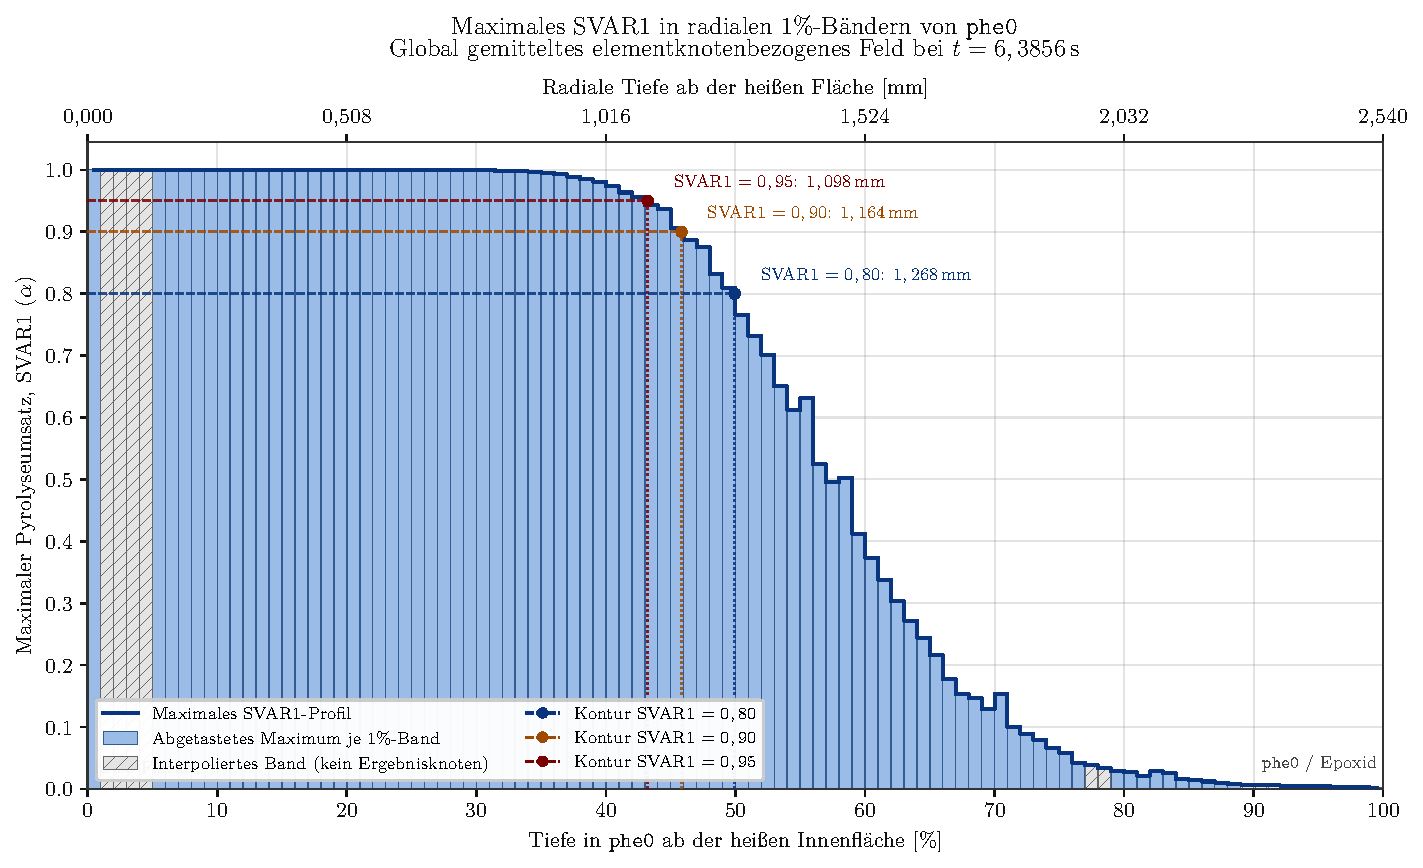
\includegraphics[width=0.98\textwidth]{../analysis/svar1_radial_profile_1pct_de.pdf}
\caption{Maximal \code{SVAR1} in einprozentigen Radialbändern von \code{phe0} im letzten konvergierten Zustand. Schraffierte Bänder enthalten keinen Ergebnisknoten und werden durch lineare Interpolation gefüllt.}
\label{fig:sim1-svar1-radial-de}
\end{figure}

Abbildung~\ref{fig:sim1-svar1-radial-de} zeigt die maximale radiale Hülle des global gemittelten Elementarknotenfeldes. Das globale Maximum erreicht \(\alpha=1\): Die Zone in der Nähe des heißen Gesichts wird vollständig nach dem kinetischen Gesetz umgewandelt. Dies bedeutet nicht, dass das Zeichen entfernt wurde oder dass eine Lücke erstellt wurde.

Die Isokonversionstiefen sind in Tabelle~\ref{tab:sim1-front-results} angegeben. Der Bereich mit mindestens 95\% erreicht \SI{1.098}{mm} oder 43.2\% der Dicke von \code{phe0}; der 80\% erreicht fast genau die Hälfte der Schicht.

\begin{table}[H]
\centering
\small
\renewcommand{\arraystretch}{1.15}
\begin{tabular}{M{0.15\textwidth}M{0.22\textwidth}M{0.22\textwidth}M{0.24\textwidth}}
\toprule
\textbf{Schwellenwert \(\alpha_c\)} &
\textbf{Tiefe \(d_{\alpha_c}\) (mm)} &
\textbf{Fraktion von \code{phe0}} &
\textbf{Scheingeschwindigkeit \(d_{\alpha_c}/t\) (\si{mm.s^{-1}})} \\
\midrule
0.80 & 1.26845 & 49.94\% & 0.19864 \\
0.90 & 1.16440 & 45.84\% & 0.18235 \\
0.95 & 1.09800 & 43.23\% & 0.17195 \\
\bottomrule
\end{tabular}~\\[1em]
\caption{Tiefe und scheinbare mittlere Geschwindigkeit der Umwandlungsfronten.}
\label{tab:sim1-front-results}
\end{table}

Die Geschwindigkeiten in der letzten Spalte sind nur die Verhältnisse \(d_{\alpha_c}/t\). Sie gehen davon aus, dass die Kontur an der heißen Seite bei \(t=0\) beginnt und eine mittlere Eindringgeschwindigkeit seit der Zündung ergibt. Es sind keine sofortigen Frontgeschwindigkeiten. Eine strenge Vordergeschwindigkeit in \si{mm.s^{-1}} muss berechnet werden, indem die Positionen der gleichen Kontur zu mehreren gespeicherten Zeiten differenziert werden.

Ein Band in der Abbildung ist \SI{25.4}{\micro m} breit, während die mittlere radiale Dicke eines \code{phe0} Elements \SI{0.318}{mm} ist. Die Balken 100 verbessern die Lesbarkeit und Integration von Profilen, erzeugen jedoch keine physikalische Auflösung von Zellen 100. Sechzehn Bänder ohne Knoten mussten interpoliert werden; die Front-Location-Unsicherheit bleibt in der Größenordnung eines Bruchteils eines Elements und muss durch Mesh-Verfeinerung gemessen werden.

\clearpage
\subsubsection{Zeitentwicklung der Umwandlung}

\begin{figure}[H]
\centering
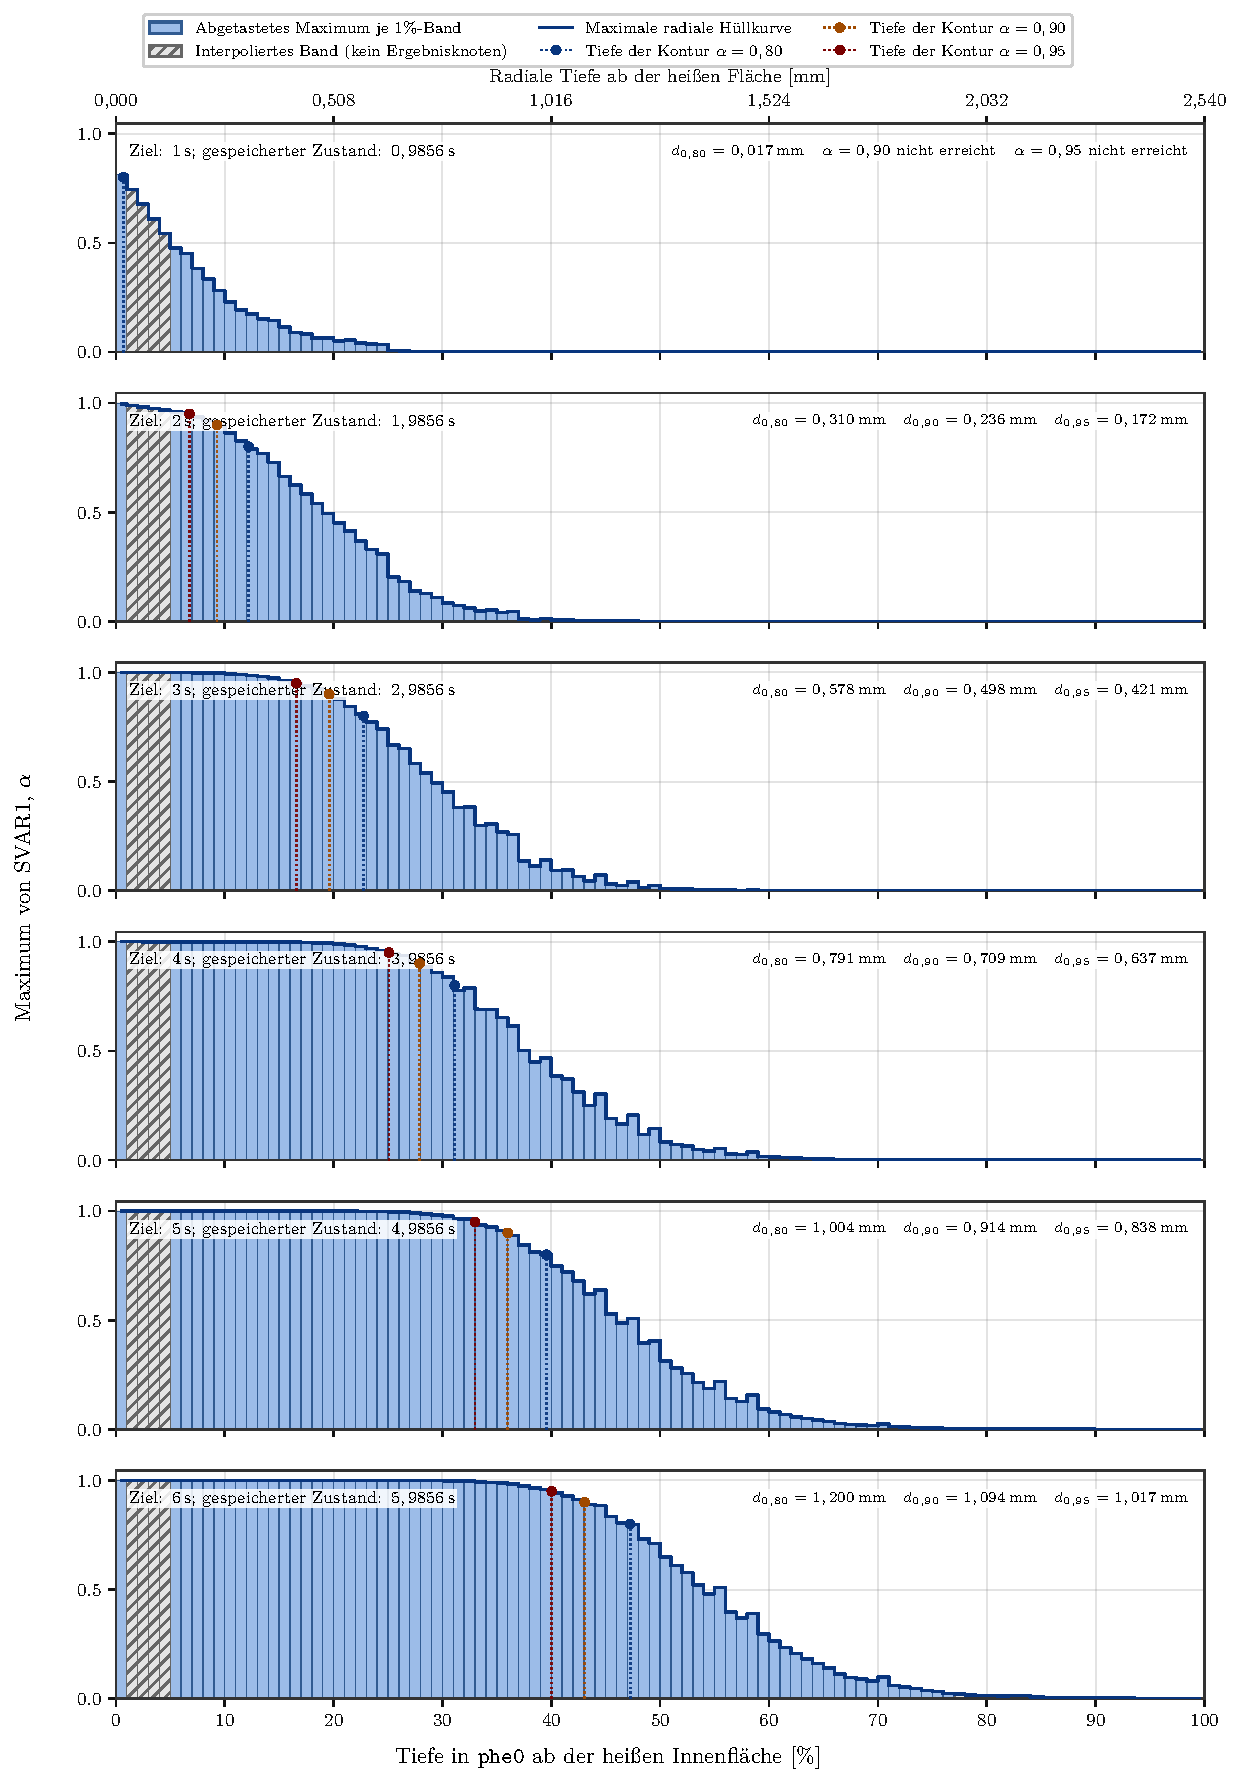
\includegraphics[height=0.80\textheight,width=0.96\textwidth,keepaspectratio]
{../analysis/svar1_time_profiles_1pct_de.pdf} \caption{Entwicklung des radialen Maximums von \code{SVAR1} in \code{phe0} für die gespeicherten Zustände, die 1 bis \SI{6}{s} am nächsten liegen. Die sechs Diagramme sind vertikal angeordnet und verwenden identische Achsen. Gestrichelte Linien und Punkte markieren die Tiefen der Isokonversionsniveaus 0.80, 0.90 und 0.95, sofern diese erreicht werden.}
\label{fig:sim1-svar1-time-de}
\end{figure}
\clearpage

Abbildung~\ref{fig:sim1-svar1-time-de} ergänzt, ohne es zu ersetzen, das Profil des letzten konvergierten Zustands in Abbildung~\ref{fig:sim1-svar1-radial-de}. Sie verwendet dieselbe Element-Knoten-Mittelung und dieselben Radialbänder von einem Prozent für die sechs gespeicherten Zustände, die \(t=1,\ldots,6~\si{s}\) am nächsten liegen. Die verfügbaren Ergebnisse liegen jeweils \SI{0.014383}{s} vor der ganzzahligen Sekunde; die tatsächlich ausgewertete Zeit ist in jedem Feld angegeben, sodass keine zeitliche Interpolation als ANSYS-Ergebnis dargestellt wird.

Tabelle~\ref{tab:sim1-svar1-time} fasst die in den Anmerkungen verwendeten Werte zusammen. Bei \SI{0.9856}{s} beträgt der Maximalwert erst \(\alpha=0.811\), und die 0.80-Kontur dringt gerade in die Schicht ein; die Niveaus 0.90 und 0.95 sind noch nicht erreicht. Dies ist eine thermische Initiationsphase und noch keine etablierte Front.

\begin{table}[H]
\centering
\small
\renewcommand{\arraystretch}{1.12}
\setlength{\tabcolsep}{4pt}
\begin{tabular}{M{0.12\textwidth}M{0.16\textwidth}M{0.14\textwidth}
M{0.15\textwidth}M{0.15\textwidth}M{0.15\textwidth}}
\toprule
\textbf{Zielzeit (s)} &
\textbf{Gespeicherte Zeit (s)} &
\textbf{\(\alpha_\mathrm{max}\)} &
\textbf{\(d_{0.80}\) (mm)} &
\textbf{\(d_{0.90}\) (mm)} &
\textbf{\(d_{0.95}\) (mm)} \\
\midrule
1 & 0.9856 & 0.81114 & 0.01691 & --- & --- \\
2 & 1.9856 & 0.99560 & 0.30979 & 0.23605 & 0.17200 \\
3 & 2.9856 & 0.99997 & 0.57818 & 0.49786 & 0.42106 \\
4 & 3.9856 & 1.00000 & 0.79069 & 0.70892 & 0.63735 \\
5 & 4.9856 & 1.00000 & 1.00433 & 0.91446 & 0.83788 \\
6 & 5.9856 & 1.00000 & 1.20013 & 1.09392 & 1.01716 \\
\bottomrule
\end{tabular}~\\[1em]
\caption{ Zeitverlauf der aus der maximalen radialen Einhüllenden berechneten Isokonversionstiefen.}
\label{tab:sim1-svar1-time}
\end{table}

Zwischen den Zuständen nahe 1 und \SI{2}{s} schreitet die 0.80 Kontur mit einer inkrementellen mittleren Geschwindigkeit von \SI{0.293}{mm.s^{-1}} voran. Diese Geschwindigkeit fällt anschließend auf \SI{0.268}{mm.s^{-1}}, dann ungefähr \SI{0.213}{mm.s^{-1}}, \SI{0.214}{mm.s^{-1}} und \SI{0.196}{mm.s^{-1}} über die aufeinanderfolgenden Intervalle. Sobald es erschienen ist, verlangsamt sich die 0.95 Kontur in ähnlicher Weise, von \SI{0.249}{mm.s^{-1}} zwischen 2 und \SI{3}{s} bis \SI{0.179}{mm.s^{-1}} zwischen 5 und \SI{6}{s}. Der allgemeine Trend ist daher eine sich verlangsamende Front mit einer kleinen nicht monotonen Variation, die mit den Teilschritten, der Knotenglättung und der radialen Maschenauflösung übereinstimmt.

Die Profile zeigen auch, dass es keine unendlich dünne Pyrolysegrenzfläche gibt: Eine breite Übergangszone trennt die fast vollständig konvertierte Kohle von noch jungfräulichem Material. Nahe \SI{6}{s} liegt die 0.95-Kontur bei \SI{1.017}{mm}, die 0.80-Kontur bei \SI{1.200}{mm}, und die messbare Umrechnung geht wesentlich weiter. Im letzten verfügbaren Zustand \SI{6.3856}{s} erreichen diese Tiefen \SI{1.098}{mm} bzw. \SI{1.268}{mm}, was den Trend der sechs Panels ohne Diskontinuität verlängert.

Für das Design verbirgt daher eine einzelne \(d/t\) Geschwindigkeit sowohl die Initiationsverzögerung als auch die nachfolgende Verlangsamung. Jede Extrapolation bis zum Ende des Brennens muss die gewählte Umwandlungsschwelle angeben und mindestens eine kürzliche inkrementelle Geschwindigkeit verwenden, anstatt die Umwandlung, die Verkohlungstiefe und die geometrische Rezession zu verschmelzen. Da jede Kurve eine maximale radiale Hüllkurve ist, bleibt sie für die rekonstruierte Umwandlung konservativ, stellt jedoch weder einen Volumenmittelwert noch eine direkt gemessene Abtragstiefe dar.

\subsubsection{Lokale Pyrolyserate \code{SVAR2}}

\code{SVAR2} ist eine lokale Umwandlungsrate in \si{s^{-1}}, die sich von der geometrischen Geschwindigkeit in Tabelle~\ref{tab:sim1-front-results} unterscheidet. Das globale Maximum über den Partitionen mit \code{phe0} ist
\[
\boxed{\dot\alpha_\mathrm{max}=\SI{0.326660}{s^{-1}}}
\]
Es tritt \SI{1.44221}{mm} vom heißen Gesicht oder 56.78\% durch die Dicke auf, wobei \(\alpha=0.54721\) und \(T=\SI{956.67}{\degreeCelsius}=\SI{1229.82}{K}\). Diese Position ist physikalisch konsistent: In der Nähe der Oberfläche ist der Faktor \(1-\alpha\) fast Null, weil das Material bereits umgewandelt ist; weiter in das Material ist die Temperatur zu niedrig, um das Arrhenius-Gesetz schnell zu aktivieren. Die maximale Rate liegt daher in der Übergangszone.

Im letzten Unterschritt \SI{0.05}{s} entspricht dieses Maximum \(\Delta\alpha\simeq0.01633\), deutlich unterhalb der numerischen Grenze von 0.05. Das Kriterium \code{UserMatTh} erzwingt daher keine zusätzliche Reduktion des letzten Inkrements. An diesem Punkt,
\[
k_r=\frac{\dot\alpha}{1-\alpha}=\SI{0.7214}{s^{-1}}, \qquad \tau_r=k_r^{-1}=\SI{1.386}{s}.
\]
Wenn die Temperatur künstlich konstant gehalten würde, würde es ungefähr \SI{3.05}{s} dauern, um von \(\alpha=0.547\) zu \(\alpha=0.95\) fortzuschreiten. Die lokale Temperatur ändert sich in der Realität immer noch, so dass diese charakteristische Zeit keine Extrapolation zum Ende des Brennens ist.

Mit \(\rho_v-\rho_c\simeq\SI{550}{kg.m^{-3}}\) bei dieser Temperatur wäre die maximale lokale Quelle, die für die Simulation vorgeschlagen wird 2
\[
\dot\omega'''_{g,\max}\simeq (\rho_v-\rho_c)\dot\alpha_\mathrm{max}=\SI{180}{kg.m^{-3}.s^{-1}}.
\]
Die bereits durch Simulation 1 aufgebrachte massenspezifische Wärmesenke ist lokal \(-\Delta H_p\dot\alpha\simeq-\SI{136.5}{kW.kg^{-1}}\). Die Gaserzeugung ist daher potenziell bedeutsam, aber ihr Transport, Druck und Wärmeaustausch werden im aktuellen Modell nicht gelöst.

\clearpage
\subsubsection{Zeitentwicklung der Lokalrate}

\begin{figure}[H]
\centering
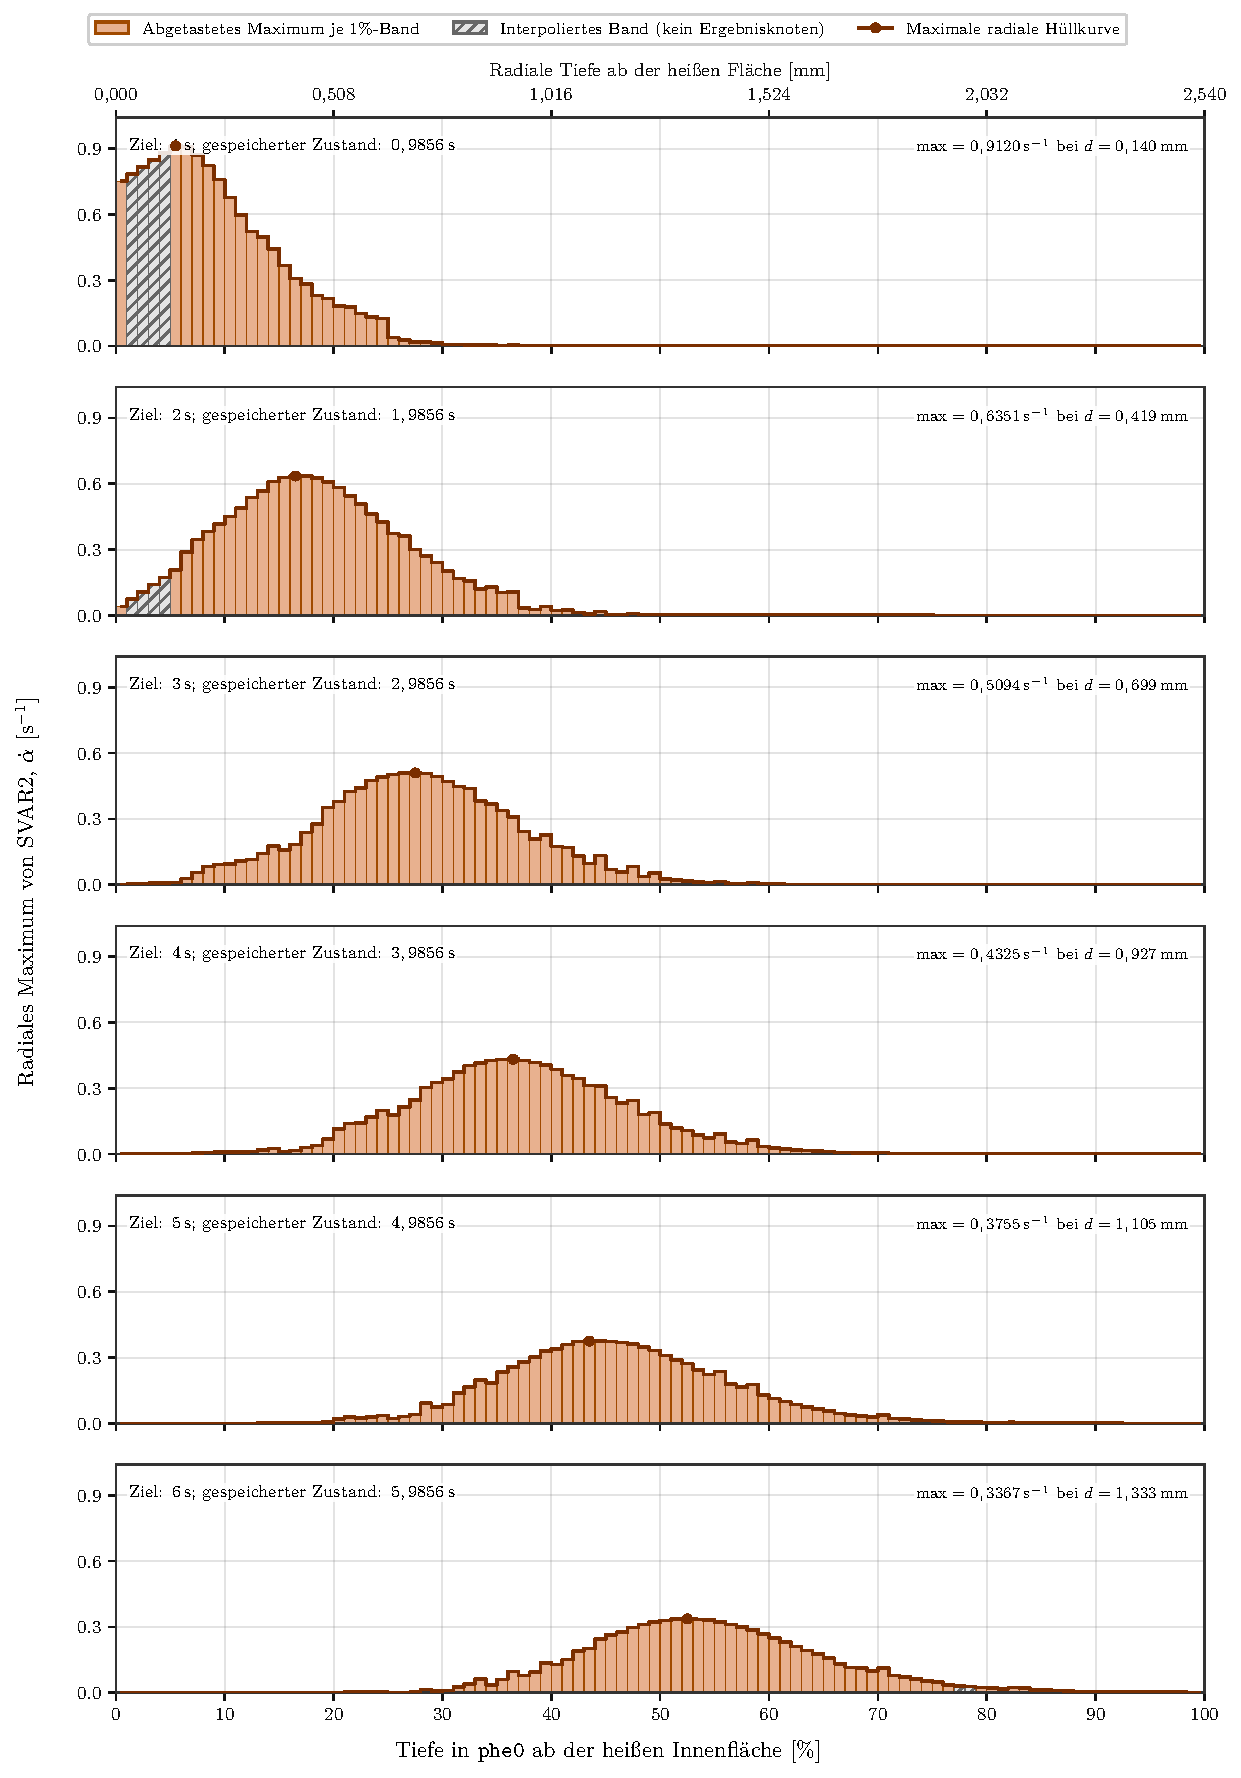
\includegraphics[height=0.80\textheight,width=0.96\textwidth,keepaspectratio]
{../analysis/svar2_radial_time_profiles_1pct_de.pdf} \caption{Entwicklung des radialen Maximums von \code{SVAR2} in \code{phe0} für die gespeicherten Zustände, die 1 bis \SI{6}{s} am nächsten liegen. Jedes Feld verwendet dieselbe vertikale Skala; schraffierte Bänder enthalten keinen Ergebnisknoten und werden linear interpoliert.}
\label{fig:sim1-svar2-time-de}
\end{figure}
\clearpage

Abbildung~\ref{fig:sim1-svar2-time-de} wendet auf \code{SVAR2} dieselbe Zeitstudie wie Abbildung~\ref{fig:sim1-svar1-time-de} an. Tabelle~\ref{tab:sim1-svar2-time} zeigt sowohl die Abnahme der Maximalrate als auch ihre Wanderung nach innen. Zwischen den Zuständen nahe 1 und \SI{6}{s} sinkt das Maximum um 63.1\% von \SI{0.9120}{s^{-1}} auf \SI{0.3367}{s^{-1}}, während seine Tiefe von \SI{0.140}{mm} auf \SI{1.333}{mm} zunimmt.

\begin{table}[H]
\centering
\small
\renewcommand{\arraystretch}{1.12}
\begin{tabular}{M{0.18\textwidth}M{0.22\textwidth}M{0.25\textwidth}M{0.25\textwidth}}
\toprule
\textbf{Zielzeit (s)} &
\textbf{Gespeicherte Zeit (s)} &
\textbf{\(\dot\alpha_\mathrm{max}\) (\si{s^{-1}})} &
\textbf{Tiefe des Maximums (mm)} \\
\midrule
1 & 0.9856 & 0.9120 & 0.140 \\
2 & 1.9856 & 0.6351 & 0.419 \\
3 & 2.9856 & 0.5094 & 0.699 \\
4 & 3.9856 & 0.4325 & 0.927 \\
5 & 4.9856 & 0.3755 & 1.105 \\
6 & 5.9856 & 0.3367 & 1.333 \\
\bottomrule
\end{tabular}~\\[1em]
\caption{ Zeitwanderung der maximalen radialen Pyrolyserate.}
\label{tab:sim1-svar2-time}
\end{table}

Die Flugbahn ist keine geometrische Rezession. Es identifiziert den Ort, an dem das Produkt aus dem Arrhenius-Faktor und der verbleibenden jungfräulichen Fraktion am größten ist. Das heiße Gesicht sättigt schnell, so dass \(1-\alpha\) dort fast Null wird; das Maximum von \(\dot\alpha\) bewegt sich dann zu tieferem Material, das noch teilweise jungfräulich, aber ausreichend heiß ist. Die Abnahme des Maximums spiegelt die thermische Dämpfung mit der Tiefe wider, nicht die Beendigung der Pyrolyse. Es erklärt auch, warum die Gasquelle in Simulation 2 volumetrisch und mobil sein muss: Nur die Oberflächenrate zu verwenden, würde die Produktion in der Übergangszone nach den ersten Sekunden stark unterschätzen.

\subsubsection{Axiale Abhängigkeit von der heißen inneren Oberfläche}

Die axiale Koordinate wird von der unteren Ebene der Maschenscheibe, \(y=\SI{0.9144}{m}\), über deren \SI{50}{mm} Länge gemessen. In jedem einprozentigen Axialband behalten die folgenden Zahlen das Maximum über Knoten auf der heißen inneren Oberfläche von \code{phe0}. Diese Einschränkung vermeidet es, ein Band ohne Oberflächenknoten durch einen kalten Knoten zu ersetzen, der tiefer im Material liegt. Werte werden mit der nativen Elemental-Knoten-Mittelung von DPF und dann durch Zusammenführen doppelter globaler Knoten an DMP-Grenzen erhalten. 83 der 100-Banden werden direkt abgetastet; die anderen 17 sind eindeutig schraffiert und zwischen ihren Nachbarn interpoliert.

\clearpage
\begin{figure}[H]
\centering
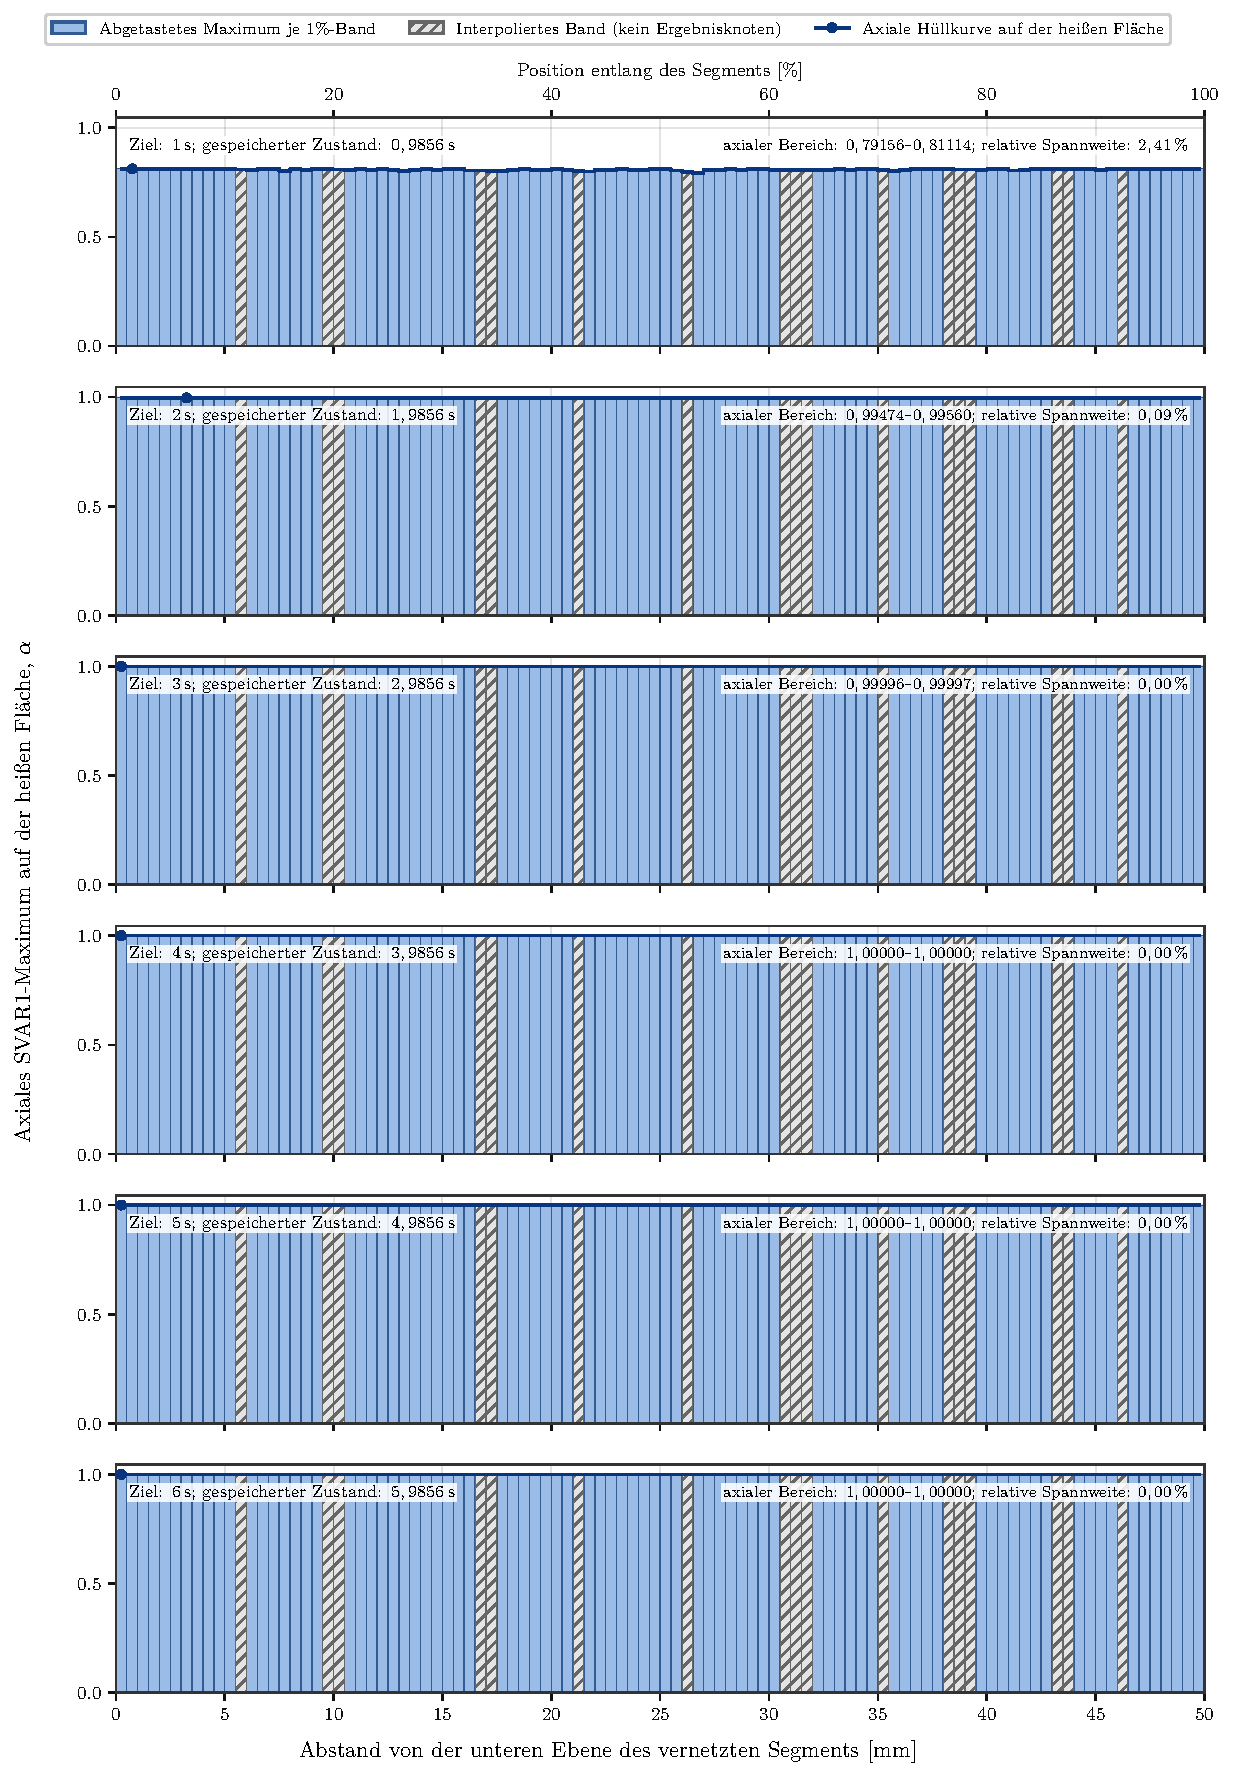
\includegraphics[height=0.80\textheight,width=0.96\textwidth,keepaspectratio]
{../analysis/svar1_axial_time_profiles_1pct_de.pdf} \caption{Axiale Abhängigkeit von \code{SVAR1} auf der heißen Innenfläche von \code{phe0}, gemessen von der unteren Ebene des vernetzten Abschnitts. Alle sechs Felder verwenden dieselbe Skala \(0\leq\alpha\leq1\).}
\label{fig:sim1-svar1-axial-de}
\end{figure}
\clearpage

\begin{figure}[H]
\centering
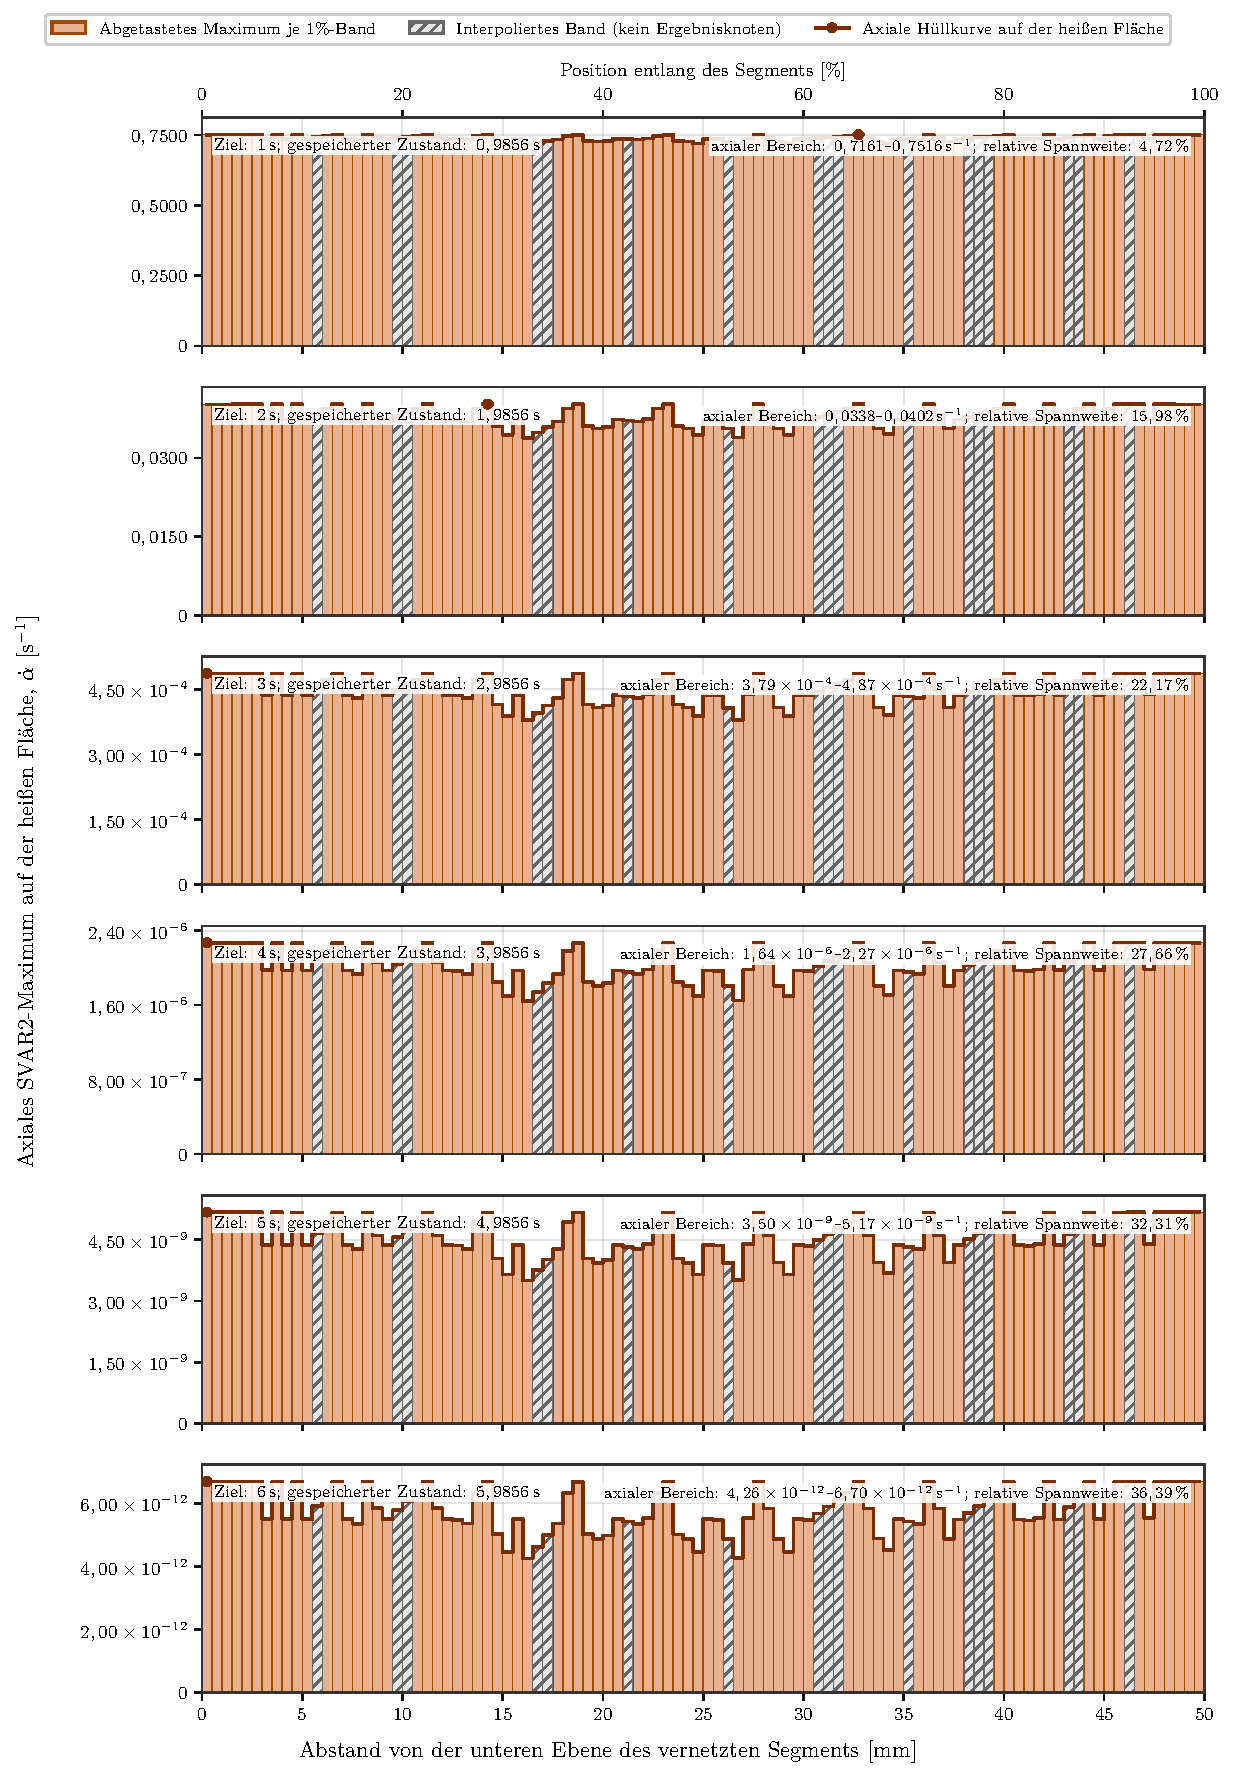
\includegraphics[height=0.80\textheight,width=0.96\textwidth,keepaspectratio]
{../analysis/svar2_axial_time_profiles_1pct_de.pdf} \caption{Axiale Abhängigkeit von \code{SVAR2} auf der heißen Innenfläche von \code{phe0}. Die vertikale Skala ist in jedem Feld unabhängig, sodass die kleinen späten Raten sichtbar bleiben; zu vergleichen sind die Absolutwerte und nicht die relativen Kurvenhöhen der Felder.}
\label{fig:sim1-svar2-axial-de}
\end{figure}
\clearpage

Abbildung~\ref{fig:sim1-svar1-axial-de} zeigt eine nahezu gleichmäßige Oberflächenkonversion. Bei \SI{0.9856}{s} reicht \(\alpha\) von 0.79156 bis 0.81114, eine relative Spanne von 2.41\%. Bei \SI{1.9856}{s} verengt sich der Bereich auf 0.99474-0.99560; bei \SI{2.9856}{s} ist es 0.999959-0.999968. Das heiße Gesicht wird numerisch vollständig aus dem Zustand nahe \SI{4}{s} konvertiert. Dies bedeutet "char voll geformt" gemäß der Zustandsvariablen, nicht "Material entfernt".

Abbildung~\ref{fig:sim1-svar2-axial-de} liefert die ergänzenden Informationen. Die Rate an der heißen Oberfläche liegt nahe \SI{1}{s} noch bei \(\SIrange{0.7161}{0.7516}{s^{-1}}\), fällt nahe \SI{2}{s} auf \(\SIrange{0.03382}{0.04025}{s^{-1}}\) und nahe \SI{3}{s} auf \(\SIrange{3.79e-4}{4.87e-4}{s^{-1}}\). Nahe \SI{4}{s} fällt sie unter \SI{2.3e-6}{s^{-1}} und ist danach praktisch null. Dieser starke Abfall ist die erwartete Folge des Faktors \(1-\alpha\): An der Oberfläche ist fast kein neues Material mehr umzuwandeln, während Abbildung~\ref{fig:sim1-svar2-time-de} bestätigt, dass die volumetrische Front tiefer im Material aktiv bleibt.

Die relative axiale Spanne von \code{SVAR2} steigt von 4.72\% bei \SI{1}{s} zu 36.39\% bei \SI{6}{s}, aber diese Zunahme ist irreführend, wenn man sie allein liest: Der Nenner ist um etwa elf Größenordnungen gefallen. Späte Schwankungen sind daher im absoluten Wert vernachlässigbar und spiegeln meist Mesh, Knotenglättung und numerische Sättigung wider. Unter den gleichmäßigen Randbedingungen dieser zentralen Schicht bestätigen beide Figuren die Annahme eines nahezu achsgleichförmigen Verhaltens. Sie unterstützen die zukünftige Verwendung eines viel billigeren rotationssymmetrischen Modells für den zentralen Bereich, sagen aber nichts über die Enden, die Düse, die Gelenke oder echte Verbrennungsflussvariationen aus.

\subsubsection{Bandbreite der Umwandlung und mögliche Ausgasung}

Zwei einfache Rekonstruktionen bieten eine Größenordnung ohne Anspruch auf eine statistische Unsicherheit. Die untere Rekonstruktion setzt \(\alpha=0.95\) zwischen dem heißen Gesicht und der Kontur bei \SI{1.098}{mm}, dann \(\alpha=0\) darüber hinaus. Die Berücksichtigung der zylindrischen Geometrie ergibt \(\bar\alpha_\mathrm{low}=0.408\). Die Integration der maximalen Hüllkurve der 100-Bänder ergibt \(\bar\alpha_\mathrm{high}=0.581\). In Tabelle~\ref{tab:sim1-mass-bracket} wird dann die nominale Gasausbeute \(Y_g=0.47\) verwendet.

\begin{table}[H]
\centering
\small
\renewcommand{\arraystretch}{1.15}
\begin{tabular}{L{0.31\textwidth}M{0.20\textwidth}M{0.20\textwidth}M{0.18\textwidth}}
\toprule
\textbf{Rekonstruktion} &
\(\boldsymbol{\bar\alpha}\) &
\textbf{ Äquivalente umgerechnete Dicke} &
\textbf{Potenzielles Gas} \\
\midrule
Unten: 95\% step front & 0.408 & \SI{1.04}{mm} &
\SI{0.943}{kg} Vollmotor; \SI{25.8}{g} Scheibe \\
Obere: maximale radiale Hülle & 0.581 & \SI{1.48}{mm} &
\SI{1.340}{kg} Vollmotor; \SI{36.6}{g} Scheibe \\
\bottomrule
\end{tabular}~\\[1em]
\caption{Ingenieurhalterung für Umwandlung und potenzielle Gasmasse bei \(t=\SI{6.3856}{s}\).}
\label{tab:sim1-mass-bracket}
\end{table}

Diese Werte gehen davon aus, dass das Profil über den gesamten Umfang und die gesamte Länge repräsentativ ist, und verwenden dann die vollständige \code{phe0} Masse von \SI{4.911}{kg}. Im vermaschten Modell ist die Länge nur \SI{50}{mm} und die entsprechende Anfangsmasse ist ungefähr \SI{0.134}{kg}. Die obere Rekonstruktion verwendet radiale Maxima und ist absichtlich konservativ für einen Durchschnitt. Die niedrigere Rekonstruktion ist keine mathematische Bindung an 3 D Lösung, weil die Figur keine Umfangs- und Axialminima enthält. Schließlich ist "potentielle Gasmasse" die Masse, die nach dem Dichtegesetz freigesetzt würde; der Löser zeigt nicht, dass diese Masse tatsächlich den Feststoff verlassen hat.

\subsubsection{Physikalische Folgen und Auswirkungen auf die Motorauslegung}

\begin{enumerate}[leftmargin=2.2em,label=\textbf{\arabic*.}]
\item \textbf{Innerliner margin.} Eine Dicke von ungefähr \SIrange{1.10}{1.27}{mm} ist bereits 80-95\% umgerechnet, und das Maximum \code{SVAR2} liegt bei \SI{1.44}{mm}. Die Front bleibt aktiv und rückt in Richtung Epoxid vor. Die Differenz \(2.54-d_{\alpha_c}\) kann nicht direkt als Ablationsrand behandelt werden, zeigt aber, dass die erste Schicht vor dem beabsichtigten Ende des Brennens stark belastet ist.

\item \textbf{Kritische Epoxidbedingung.} Das Modell prognostiziert \SI{453}{\degreeCelsius} in einer Epoxidschicht, die dennoch als inert und gebunden angenommen wird. Dieser Wert liegt außerhalb des Bereichs seiner thermischen Eigenschaftstabelle. Das Modell kann daher nicht feststellen, dass entweder die \code{phe0--epo} oder \code{epo--phe1} Bindung überlebt. Eine Charakterisierung des Epoxids, eine dickere thermische Barriere oder ein Hochtemperaturkleber müssen berücksichtigt werden, bevor die Verklebung als sicher behandelt werden kann.

\item \textbf{Aluminium nur kurzfristig geschützt.} Die ideale zentrale Scheibe hält das Aluminium nahe \SI{22}{\degreeCelsius} bei \SI{6.39}{s}. Dies ist günstig, schließt jedoch keine verzögerte Erwärmung nach dem Abschalten, Wärmebrücken oder Düsen- und Endbereiche ein. Eine vorübergehende Abkühlphase muss hinzugefügt werden, um nach der verzögerten maximalen Aluminiumtemperatur zu suchen.

\item \textbf{Nicht vernachlässigbare Ausgasung.} Der Wert \code{SVAR2} impliziert eine hohe lokale Gasquelle. Ohne den porösen Transport kann die Simulation den Innenkohlendruck, die Blaskühlung oder das gasunterstützte Delaminationsrisiko nicht vorhersagen. Diese Phänomene motivieren direkt Simulation 2.

\item \textbf{Vorderauflösung.} Acht Elemente über \SI{2.54}{mm} bieten nur drei bis vier Elementschichten über die Hauptübergangszone. Läufe mit 16 und dann 24 Radialschichten sollten \(d_{0.8}\), \(d_{0.95}\), \(\dot\alpha_\mathrm{max}\) und die Epoxidtemperatur vergleichen.

\item \textbf{Beschränkung der zentralen Schicht.} Das \SI{50}{mm}-Mesh stellt einen einheitlichen Mittellängenbereich dar, nicht jedoch Endbereichsflusskonzentrationen oder Leitungspfade. Die Massen in Tabelle~\ref{tab:sim1-mass-bracket} können nur dann auf den Vollmotor skaliert werden, wenn die axiale Gleichmäßigkeit überprüft wird.
\end{enumerate}

\subsubsection{Vergleich mit der Realität und weiteres Vorgehen}

Es gibt derzeit keine TGA / DSC / LFA-Kurve für das tatsächlich hergestellte Phenol, keine Thermoelementaufzeichnung von einem Motorfeuer und keine Messung der Masse, der Kohletiefe oder der Rezession nach dem Brand. Es wäre daher falsch, eine quantitative Übereinstimmung mit der Realität zu behaupten. Der verfügbare Vergleich betrifft die Mechanismen: NASA-verifizierte Verkohlungsablatormodelle umfassen Leitung, Zersetzung, Pyrolyse-Gasfluss, Gas-Feststoff-Wärmeaustausch, thermochemische Erosion und Oberflächenbewegung ~\cite{ewing2013,amar2010,amar2016}. Simulation 1 stellt nur Leitung, lokale Kinetik, jungfräuliche/kohle Eigenschaften und die endotherme Senke dar.

\begin{table}[H]
\centering
\footnotesize
\renewcommand{\arraystretch}{1.18}
\begin{tabular}{L{0.25\textwidth}L{0.34\textwidth}L{0.31\textwidth}}
\toprule
\textbf{Annahme oder Auslassung} & \textbf{Fehlender physikalischer Effekt} &
\textbf{Like Bias} \\
\midrule
Konstante \(T_g\) und \(h_\mathrm{in}\) aus \(t=0\) &
Keine Zündrampe oder Druckabfall &
Hohe Tendenz, wenn das wirkliche Feuern Rampen hat; unbekannte Richtung, wenn die tatsächliche
Flux oder Partikelstrahlung ist höher. \\
Kein mobiles Pyrolysegas &
Kein Wandblasen, advektierte Enthalpie oder Porendruck &
Oft eine hohe Tendenz zum Eindringen von Nettowärme, aber nicht eine einseitige Grenze
für Innentemperatur. \\
Keine Oxidation, Erosion oder Partikel &
Kein thermochemischer oder mechanischer Kohleverbrauch &
Untergrenze für Rezession und geometrischen Massenverlust. \\
Char beibehalten und keine Elemente entfernt &
Die Oberfläche geht nie zurück &
Genau null berechnete Rezession: eine modellhafte Untergrenze. \\
Perfekt gebondete Kontakte &
Keine Lücke, Delamination oder sich entwickelnde Resistenz &
Hohe Tendenz zur idealen Wärmeübertragung, aber eine zu optimistische Sicht auf
Haftfestigkeit. \\
Unkalibrierte Eigenschaften und Kinetik &
Unbekannter Gehalt, Fasern, Ernteausbeute und Mehrfachreaktionen &
Keine vertretbare Verzerrungsrichtung; diese Unsicherheit kann alle anderen dominieren. \\
Maximales Radialprofil &
Umschlag statt Volumendurchschnitt &
Engineering-Obergrenze für die rekonstruierte mittlere Umrechnung. \\
\bottomrule
\end{tabular}~\\[1em]
\caption{Erwartete Richtung der Hauptverzerrungen relativ zu einer realen Zündung.}
\label{tab:sim1-reality-bounds}
\end{table}

Für \emph{geometrische Rezession} ist die Untergrenze des aktuellen Modells daher \SI{0}{mm}. Eine einfache obere Grenze geht davon aus, dass die gesamte äquivalente umgerechnete Dicke, etwa \SIrange{1.0}{1.5}{mm}, ebenfalls abgestreift wird; sie ist absichtlich stark, weil 52--56\% der kondensierten Masse gemäß den aktuellen Tabellen als Char verbleibt. Die Realität kann zwischen diesen Werten liegen, wenn die Kohle teilweise befestigt bleibt, aber eine starke Oxidation oder mechanische Erosion kann diese Halterung ungültig machen. Nur eine instrumentierte Feuerung und Nachbrandmessung kann sie schließen.

Die Validierungsprioritäten sind daher: (i) charakterisieren die tatsächliche Phenol und Epoxy durch TGA, DSC und LFA, Methoden explizit von der NASA für Restmasse, Wärmekapazität und thermische Diffusivität Messungen ~ \cite{nasa-testing}; (ii) messen \(T_g(t)\), Druck und Temperaturen an den Grenzflächen und auf dem Aluminium während eines Brennens; (iii) messen Masse, Restdicke und Kohle Tiefe nach dem Brennen; (iv) erweitern die Berechnung zu \SI{7}{s} und dann durch Abkühlung; und (v) führen Sensitivitätsstudien auf \(h_\mathrm{in}\), \(A\), \(E_a\), \(\Delta H_p\), Kohleeigenschaften, Kontakte, Zeitschritt und Mesh.

% ============================================================================
\clearpage
\section{Simulation 2: Ausgasung und Element Deaktivierung in Mechanical}

\subsection{Vorgeschlagene Theorie und Ableitung}

\subsubsection{Feststoffmassenbilanz und Gaserzeugung}

Die Simulation 2 behält die in der Simulation verwendete Kinetik 1 bei, unterscheidet jedoch den festen Rückstand von den gasförmigen Produkten. Über ein Anfangsvolumen ist der Verlust der kondensierten Phase Masse die Gasquelle:
\begin{equation}
  \frac{\pd\rho_s}{\pd t}=-\dot\omega'''_g,
  \qquad
  \dot\omega'''_g=(\rho_v-\rho_c)\dot\alpha.
  \label{eq:solid-mass-sim2}
\end{equation}
Die endgültige Gasausbeute des Einreaktionsmodells ist daher
\begin{equation}
  Y_g=\frac{\rho_v-\rho_c}{\rho_v}=1-\frac{\rho_c}{\rho_v}.
  \label{eq:gas-yield}
\end{equation}
Bei den aktuellen Tabellen reicht \(Y_g\) von 0.44 bis 0.48. Ein Nominalwert von \(Y_g=0.47\) stimmt mit dem Modell überein, muss jedoch mit der von TGA gemessenen Restmasse bestätigt werden.

In einem vollständigen Porenablator-Modell wird die Erhaltung der Gasmasse als
\begin{equation}
  \frac{\pd(\phi\rho_g)}{\pd t}
  +\vect\nabla\cdot(\rho_g\vect u_g)=\dot\omega'''_g,
  \label{eq:gas-mass-full}
\end{equation}
Dabei ist \(\phi\) die Porosität und \(\vect u_g\) die oberflächliche Geschwindigkeit. Für langsames Fließen durch die Kohle geben Darcys Gesetz und das Idealgasgesetz
\begin{equation}
  \vect u_g=-\frac{K(\alpha,T)}{\mu_g}\vect\nabla p_g,
  \qquad
  \rho_g=\frac{p_g M_g}{R T_g}.
  \label{eq:darcy-ideal}
\end{equation}
Antwortcodes für Ablative-Materialien wie CHAR lösen gekoppelte Formen dieser Massen- und Energiebilanz ~\cite{amar2010,amar2016,ewing2013}. Ein Standard-Thermoelement in Mechanical hat jedoch keinen Druckfreiheitsgrad. Folglich kann \code{UserMatTh} Gleichung~\eqref{eq:gas-mass-full} nicht von selbst lösen. Der Verbleib in Mechanical erfordert daher entweder ein wesentlich komplexeres benutzerdefiniertes Multiphysik-Element oder ein Modell reduzierter Ordnung.

\subsubsection{Mit Mechanical kompatibler reduzierter Radialabschluss}

Das vorgeschlagene Modell geht davon aus, dass die in \code{phe0} erzeugten Gase schnell in Richtung der heißen Wand entweichen und dass ihre Akkumulation vernachlässigbar ist. In der zylindrischen Achsensymmetrie wird der Gasmassenfluss, der die Oberfläche im Radius \(r_s\) erreicht, dann direkt durch Integration der Quelle erhalten:
\begin{equation}
  \boxed{\dot m''_g(r_s)=\frac{1}{r_s}
  \int_{r_s}^{R_0}\dot\omega'''_g(r)\,r\,\dd r,}
  \label{eq:radial-gas-flux}
\end{equation}
wobei \(R_0\) die äußere Grenze von \code{phe0} ist. Dieser Ausdruck folgt aus dem Saldo \(2\pi r_sL\dot m''_g=\int_{r_s}^{R_0}2\pi rL \dot\omega'''_g\dd r\). Es konserviert die Gesamtgasmasse, auch wenn der Druck nicht explizit gelöst wird.

Das Gas trägt eine sensible Enthalpie. Eine minimale lokale Schließung fügt der Festenergiegleichung den folgenden Term hinzu:
\begin{equation}
  \dot q_{m,g}=-\frac{\dot\omega'''_g}{\rho_s}
  c_{p,g}(T-T_\mathrm{ref}).
  \label{eq:gas-local-sink}
\end{equation}
Dieser Begriff muss nur verwendet werden, wenn \(\Delta H_p\) diese Enthalpie nicht bereits enthält; andernfalls würde er zweimal gezählt. Eine getreuere Formulierung fügt \(-\vect\nabla\cdot(\dot m''_g h_g)\) zur Energiebilanz hinzu, wie es in Material-Antwort-Modellen ~\cite{ewing2013,amar2010} getan wird.

\subsubsection{Verringerung des konvektiven Wärmeflusses durch Blasen}

Das Ausgasen in die Kammer erzeugt eine Blasströmung, die der Wärmeübertragung entgegensteht. Für einen stetigen, planaren Gasfilm mit konstanten Eigenschaften ist die quellenfreie Energiegleichung
\begin{equation}
  \dot m''_g c_{p,g}\frac{\dd T}{\dd y}
  =k_g\frac{\dd^2T}{\dd y^2}.
\end{equation}
Die Integration zwischen der Wand und dem äußeren Rand der Folie und die Angabe der Schichtdicke in Bezug auf den No-Blow-Koeffizienten \(h_0=k_g/\delta\) ergibt die klassische Korrektur in der Form
\begin{equation}
  B_h=\frac{\dot m''_g c_{p,g}}{h_0},\qquad
  F(B_h)=\frac{B_h}{\exp(B_h)-1},
\end{equation}
\begin{equation}
  \boxed{q''_\mathrm{conv}=h_0F(B_h)(T_g-T_s).}
  \label{eq:blowing}
\end{equation}
Da \(F(0)=1\) und \(F(B_h)<1\) für \(B_h>0\), stellt das Modell die aktuelle Konvektionsbedingung in Abwesenheit von Ausgasung wieder her und reduziert schrittweise den Wärmefluss, wenn die Gasproduktion zunimmt. Dieses Gesetz ist ein technischer Abschluss; es ersetzt keine Grenzschichtberechnung und muss gegen Kammerdruck, Treibmittelzusammensetzung und Testdaten kalibriert werden.

\subsubsection{Oberflächenbilanz, Rezession und Element-Deaktivierungskriterium}

Die Pyrolyse erzeugt Kohle; sie entfernt diese Kohle nicht automatisch. Rezession erfordert einen zweiten Mechanismus - Oxidation, Sublimation oder mechanische Erosion - und eine Oberflächenenergiebilanz:
\begin{equation}
  q''_\mathrm{conv}+q''_\mathrm{rad}
  =q''_\mathrm{cond}+\dot m''_g\Delta h_g
   +\dot m''_\mathrm{abl}H_\mathrm{eff}.
  \label{eq:surface-balance}
\end{equation}
In Ermangelung ausreichender chemischer Daten wird das folgende begrenzte, energiekontrollierte Gesetz vorgeschlagen:
\begin{equation}
  \dot m''_\mathrm{abl}=
  \max\left[0,
  \frac{q''_\mathrm{conv}+q''_\mathrm{rad}-q''_\mathrm{cond}
  -\dot m''_g\Delta h_g}{H_\mathrm{eff}}\right],
  \qquad
  \dot s=\frac{\dot m''_\mathrm{abl}}{\rho_c}.
  \label{eq:recession}
\end{equation}
Die Rezessionstiefe ist \(s(t)=\int_0^t\dot s\dd t\). Die \code{phe0} Elemente sind in radialen Bändern angeordnet; ein Band wird nur deaktiviert, wenn \(s\) seine kumulative Dicke überschreitet. Das Kriterium ist daher die integrierte Rezession, möglicherweise kombiniert mit \(\alpha\ge0.99\), aber niemals \(\alpha=1\) allein.

In MAPDL multipliziert \code{EKILL} den Beitrag eines Elements mit einem Faktor nahe null; das Element bleibt im Netz. Ein deaktiviertes thermisches Element trägt weder Wärmekapazität noch aufgebrachte Lasten bei, und seine Zustandsvariablen werden bei der Deaktivierung zurückgesetzt~\cite{ansys-birthdeath,ansys-ekill}. Jede Restmasse und -energie muss daher vor \code{EKILL} aufgezeichnet und in die Bilanz aufgenommen werden. Nach der Deaktivierung eines Bandes müssen die heißseitigen Konvektions- und Oberflächenelemente auf die neu freigelegte Fläche übertragen werden. Bei nur acht Schichten in \code{phe0} würde die Rezession in Schritten von etwa \SI{0.318}{mm} fortschreiten. Eine belastbare Rezessionsstudie sollte 20 bis 40 Radialbänder verwenden oder nachweisen, dass das vorhandene Inkrement hinreichend klein ist.

\begin{figure}[H]
\centering
\begin{tikzpicture}[font=\sffamily\small,>=Latex,node distance=8mm and 9mm,
  block/.style={draw=B,very thick,rounded corners=7pt,fill=b!10,
    align=center,text width=34mm,minimum height=13mm},
  special/.style={draw=phenolicA,very thick,rounded corners=7pt,fill=phenolicB!20,
    align=center,text width=34mm,minimum height=13mm},
  kill/.style={draw=r,very thick,rounded corners=7pt,fill=red!8,
    align=center,text width=34mm,minimum height=13mm},
  arr/.style={-Latex,very thick,draw=black!60}]
  \node[block] (pyro) {lokale Pyrolyse\\\(\alpha,\dot\omega'''_g\)};
  \node[block,right=of pyro] (gas) {radialer Gasmassenstrom\\\(\dot m''_g\)};
  \node[special,right=of gas] (blow) {Ausblasung und Enthalpie\\\(F(B_h),\Delta h_g\)};
  \node[block,below=of blow] (surface) {Oberflächenbilanz\\\(\dot m''_\mathrm{abl}\)};
  \node[special,left=of surface] (recession) {integrierte Rezession\\\(s(t)\)};
  \node[kill,left=of recession] (ekill) {Bandschwelle überschritten\\\code{EKILL}};
  \draw[arr] (pyro)--(gas); \draw[arr] (gas)--(blow);
  \draw[arr] (blow)--(surface); \draw[arr] (surface)--(recession);
  \draw[arr] (recession)--(ekill);
  \draw[arr] (ekill.west) -- ++(-6mm,0) |- (pyro.west)
    node[pos=.25,left,align=right] {neue heiße\\Oberfläche};
\end{tikzpicture}
\caption{Vorgeschlagene physikalische Sequenz für Simulation 2 in Mechanisch. Die Deaktivierung des Elements wird durch Rezession verursacht, nicht direkt durch SVAR1.}
\label{fig:sim2-chain}
\end{figure}

\subsubsection{Vorgeschlagene Anfangswerte und Sensitivitätsstudien}

Tabelle~\ref{tab:sim2-values} stellt einen anfänglichen Parametersatz für die Prototypentwicklung bereit, nicht für die Qualifizierung. Die Permeabilitätswerte stammen aus dem CHAR-PICA-Modell und dienen lediglich als Ersatzwerte für ein dichtes Phenolharz~\cite{amar2016}. Zu den Pyrolyseprodukten von Phenolharzen gehören unter anderem \(\mathrm{H_2}\), Wasserdampf und aromatische Kohlenwasserstoffe; ihre Zusammensetzung hängt von der Heizrate ab~\cite{bessire2023}. Die Darstellung durch eine einzige Pseudospezies ist daher eine starke Vereinfachung.

\begin{table}[H]
\centering
\scriptsize
\renewcommand{\arraystretch}{1.18}
\begin{tabular}{L{0.18\textwidth}M{0.16\textwidth}M{0.18\textwidth}L{0.38\textwidth}}
\toprule
\textbf{Menge} & \textbf{Vorgeschlagenes Nominal} & \textbf{ Empfindlichkeitsbereich} & \textbf{Rationale / erforderliche Messung} \\
\midrule
Gasausbeute \(Y_g\) & 0.47 & 0.44--0.50 & Abgeleitet von den aktuellen jungfräulichen/char-Dichte mit Gleichung~\eqref{eq:gas-yield}; Ersetzen mit TGA-Daten. \\
Jungfernporosität \(\phi_v\) & 0.13 & 0.05--0.20 & Abgeleitet von \(1-\rho_v/\rho_\mathrm{skeletal}\), mit \(\rho_\mathrm{skeletal}=\SI{1430}{kg.m^{-3}}\), einem historischen Phenol--Nylon-Wert~\cite{clark1972}. \\
Charporosität \(\phi_c\) & 0.55 & 0.45--0.65 & Gleiche Berechnung mit \(\rho_c=\SIrange{600}{700}{kg.m^{-3}}\); Messung durch Pyknometrie/Porosimetrie. \\
Virgin Permeabilität \(K_v\) & \(10^{-12}\ \mathrm{m^2}\) & \(10^{-14}\)--\(10^{-11}\ \mathrm{m^2}\) & PICA ``Model A''-Wert verwendet als Surrogat~\cite{amar2016}; nicht übertragbar ohne Prüfung. \\
Char Permeabilität \(K_c\) & \(10^{-10}\ \mathrm{m^2}\) & \(10^{-12}\)--\(10^{-9}\ \mathrm{m^2}\) & Gleiche Quelle; logarithmische Interpolation in Bezug auf \(\alpha\) wird empfohlen. \\
Gasviskosität \(\mu_g\) & \(4\times10^{-5}\ \mathrm{Pa\,s}\) & \(2\)--\(6\times10^{-5}\ \mathrm{Pa\,s}\) & Vorläufiger Wert für heißes Pseudogas; eine Berechnung des Gemischs ist erforderlich. \\
Molmasse \(M_g\) & \(\SI{0.024}{kg.mol^{-1}}\) & 0.018--0.030 & Pseudo-Arten, die leichte Gase und Dämpfe überspannen; aus der gemessenen Zusammensetzung berechnen. \\
Gaswärmekapazität \(c_{p,g}\) & \(\SI{1.5}{kJ.kg^{-1}.K^{-1}}\) & 1.2--2.0 & Anfänglicher Pseudogaswert; nach der Charakterisierung eine \(c_p(T,p)\) Tabelle verwenden. \\
Emissionsgrad des Verkohlungsprodukts \(\varepsilon_c\) & 0.80 & 0.70--0.90 & Historischer Ausgangswert für Phenolharz--Nylon~\cite{clark1972}; Hochtemperaturmessung erforderlich. \\
Ablationsenthalpie \(H_\mathrm{eff}\) & \(\SI{35}{MJ.kg^{-1}}\) & 20, 35 und \(\SI{50}{MJ.kg^{-1}}\) & Effektiver Rezessionsparameter. \SI{50}{MJ.kg^{-1}} ist ein historischer Sublimationsanker~\cite{clark1972}; Kalibrieren gegen Dickenverlust. \\
Bezugstemperatur \(T_\mathrm{ref}\) & \(\SI{295.15}{K}\) & fix & Konsistent mit dem Ausgangszustand. \\
Rezessionszuwachs & \(\dot s\Delta t\le0.2\Delta r\) & 0.1--0.25 \(\Delta r\) & Numerisches Kriterium, um zu verhindern, dass mehrere Bänder in einem Teilschritt gekreuzt werden. \\
\bottomrule
\end{tabular}~\\[1em]
\caption{Vorgeschlagene Anfangsparameter für Simulation 2. Sie müssen als unsichere Variablen behandelt werden, bis sie charakterisiert wurden.}
\label{tab:sim2-values}
\end{table}

Bevor eine vollständige Motorsimulation versucht wird, sind drei separate Validierungskampagnen erforderlich: (i) \mbox{TGA/DSC/LFA} Coupon-Tests für die Zersetzung, (ii) Permeabilitäts- und Gasdruckmessungen in einem beheizten Coupon für die Ausgasung und (iii) ein instrumentierter Flammen- oder Motortest für \(h_0\), Blasen und Rezession. Das Modell darf eine falsche Kammerrandbedingung nicht durch eine künstliche Anpassung von \(H_\mathrm{eff}\) kompensieren.

\subsection{Implementierung in Mechanical}

\subsubsection{Rechenarchitektur}

Simulation 2 wurde mit ANSYS Mechanical APDL 2026 R1.02 implementiert und ausgeführt. Es verwendet das validierte dreidimensionale Netz aus Simulation 1 und die native Bibliothek \code{UserMatTh} wieder. Die fünf Zustandsvariablen, die in \code{phe0} gespeichert sind, sind:
\begin{equation}
  \mathrm{SVAR1}=\alpha,\quad
  \mathrm{SVAR2}=\dot\alpha,\quad
  \mathrm{SVAR3}=\dot\omega'''_g,\quad
  \mathrm{SVAR4}=\int\dot\omega'''_g\dd t,\quad
  \mathrm{SVAR5}=\dot q_{m,g}.
\end{equation}
Das erste mechanische Befehlsobjekt konfiguriert das Benutzermaterial; das zweite treibt die Transientenschleife an. Jeder Makroschritt folgt der Sequenz
\[
\code{SOLVE}\ \longrightarrow\ \text{Gas- und Energiebilanz}\ \longrightarrow\ \text{Blowing und Rezessionsupdate}\ \longrightarrow\ \text{multiframe restart}.
\]
Nach dem ersten Makroschritt nimmt \code{ANTYPE,,REST,,,CONTINUE} explizit den letzten konvergierten Zustand wieder auf. Die Temperatur und die SVARs werden daher nicht aus \(t=0\) neu berechnet.

Die Berechnungsziele \SI{7}{s} verwenden 140 einheitliche Makroschritte von \(\Delta t=\SI{0.05}{s}\). Die \SI{2.54}{mm}-dicke innere \code{phe0}-Schicht ist in acht radiale Bänder unterteilt, von denen jede \SI{0.3175}{mm} dick ist. Der Controller verwendet \(T_g=\SI{2230.85}{\celsius}\), \(h_0=\SI{1000}{W.m^{-2}.K^{-1}}\), \(c_{p,g}=\SI{1600}{J.kg^{-1}.K^{-1}}\), \(\rho_c=\SI{600}{kg.m^{-3}}\) und \(H_\mathrm{eff}=\SI{35}{MJ.kg^{-1}}\). Ein Band wird nur deaktiviert, wenn alle drei folgenden Bedingungen erfüllt sind:
\[
  \bar\alpha\ge0.99,\qquad
  \alpha_\mathrm{min}\ge0.90,\qquad
  s\ge(i+1)\Delta r.
\]
Nachdem die Oberflächeneffektelemente installiert wurden, enthält das aktuelle Modell ungefähr 2.24 Millionen Knoten und \(7.15\times10^5\) Elemente. Die innere Oberfläche enthält 135,900 Knoten und 43,488 Oberflächeneffektelemente; das erste Kandidatenband enthält 39,808 Elemente.

\begin{table}[H]
\centering
\small
\renewcommand{\arraystretch}{1.15}
\begin{tabular}{L{0.38\textwidth}L{0.50\textwidth}}
\toprule
\textbf{Numerischer Parameter} & \textbf{Ausgeführter Wert} \\
\midrule
Version und Solver & MAPDL 2026 R1.02, nichtlineare transiente thermische Analyse \\
Parallele Ausführung & Distributed Memory, Intel MPI, 10 ranks, ein Thread pro rank \\
Zeithorizont & \SI{7}{s}, 140 Makroschritte von \SI{0.05}{s} \\
Global mesh & 2,242,327 Knoten; ungefähr 714,676 Elemente nach Einrichtung \\
Heiße Oberfläche & 135,900 Knoten; 43,488 Oberflächeneffektelemente \\
\code{phe0} Bänder & 8 Bänder, jeweils \SI{0.3175}{mm} dick \\
Persistenz & CSV-Historie bei jedem Schritt und verteilte Neustartdateien auf allen 10 Rängen \\
\bottomrule
\end{tabular}
\caption{Ausgeführte numerische Konfiguration für Simulation 2.}
\label{tab:sim2-implementation}
\end{table}

\subsubsection{Persistenz, Wiederaufnahme und Konsistenzprüfungen}

Die Datei \codepath{simulation2_history.csv} wird nach jedem Makroschritt geschlossen und im Append-Modus wieder geöffnet. Eine Datei \codepath{simulation2_state.parm} speichert die letzte gelöste Zeit, Salden, Rezession und das aktive Band. Neustart-Dateien bleiben verteilt; eine Wiederherstellung ist nur gültig, wenn die zehn rangspezifischen Sätze, der Verlauf und der Parameterzustand auf denselben Ladeschritt zeigen.

Die erste Kampagne wurde nach dem Ladeschritt 15 bei \(t=\SI{0.75}{s}\) sauber gestoppt und dann vom Ladeschritt 16 wieder aufgenommen. Die Fortsetzung stellte das Ergebnis bei \SI{0.80}{s} wieder her und verlief ohne Wiederinitialisierung der Temperatur oder der SVARs. Diese Wiederherstellung ist eine wichtige Robustheitsprüfung, da eine vollständige Berechnung mehrere Tage Wanduhrzeit erfordert. Die Kampagne wurde dann absichtlich am Juli gestoppt 23, 2026. Der Ladeschritt 130 war bei \SI{6.50}{s} konvergiert, aber die globale Ergebnismontage war noch im Gange: Der Verlauf und der Parameterzustand blieben beim Ladeschritt 129, \SI{6.45}{s} synchronisiert. Dementsprechend schließen alle endgültigen Statistiken und Zahlen den unsynchronisierten Zustand \SI{6.50}{s} aus.

Rezessionsratenstatistiken werden schreibgeschützt mit DPF aus den zehn \code{file0.rth} bis \code{file9.rth} Dateien extrahiert. Für jeden Zustand überprüft die Extraktion alle 135,900 innere Oberflächenknoten und vergleicht die Ergebniszeiten mit der Historie. Zahlen werden erst veröffentlicht, nachdem sich die verteilten Ergebnisdateien stabilisiert haben.

\subsection{Ergebnisse und Leistung von Simulation 2}

\subsubsection{Laufstatus und numerische Leistung}

Die Kampagne ist durch Benutzerentscheidung abgeschlossen. Der letzte vollständig synchronisierte Zustand ist der Ladeschritt 129 bei \(t=\SI{6.45}{s}\) oder 92.1\% der Ziel-Physikdauer. Die verbleibende \SI{0.55}{s} wurde nicht berechnet und es wird keine Extrapolation als Ergebnis dargestellt.

Die beobachtete Fortsetzung vom Ladeschritt 17 durch den Ladeschritt 129 enthält 113 synchronisierte Makroschritte und keine MAPDL-Fehler. Von diesen Schritten konvergierte 93 in zwei Gleichgewichts-Iterationen und 20 in drei. Der Ladeschritt 130 konvergiert ebenfalls in zwei Iterationen, wird aber aus der Waage ausgeschlossen, da er nicht synchronisiert wurde. Die mittlere Wandzeit pro Makroschritt ist 45.1 Minuten über der synchronisierten Fortsetzung. Sie nimmt zu, wenn die Ergebnisdateien wachsen: Über die letzten 24 Schritte ist der Median 60.3 Minuten, was ungefähr \SI{0.050}{s} simulierter Zeit pro Wanduhrstunde entspricht. In den letzten zehn Schritten erreicht der Median 67.1 Minuten, mit einem beobachteten Bereich von 59.1 bis 125.8 Minuten; die größten Werte werden in erster Linie mit der Ergebnismontage assoziiert.

Thermische Lösungszeit ist nicht die einzige dominierende Kosten. Nach jeder Konvergenz sammelt und interpretiert MAPDL die verteilten Ergebnisse; diese Phase kann derzeit ungefähr 40 Minuten dauern. Die residente Datenbankzuweisung musste automatisch von 1 zu 4~GB wachsen. Der PCG-Solver meldet auch mehr als 1,000 lineare Iterationen pro Ladeschritt und schlägt den direkten SPARSE-Solver vor. Jeder Solverwechsel muss jedoch in einem separaten kontrollierten Vergleich unter Verwendung der gleichen Mesh- und Ergebnisspeichereinstellungen ausgewertet werden.

Das Continuation Log enthält null Fehler. Die Warnung \code{RESCONTROL,DEFINE}, die besagt, dass der Befehl während eines Neustarts ignoriert wird, wiederholt sich bei jedem Makroschritt, ohne dass ein Verlust von Checkpoints beobachtet wird. Acht erste Warnhinweise betreffen Tabellen mit Materialeigenschaften, die geringfügig außerhalb der tabellarischen Bereiche bewertet wurden; diese Bereiche müssen vor der Einstufung erweitert werden, auch wenn die Warnhinweise die Konvergenz nicht verhindert haben.

\begin{table}[H]
\centering
\small
\renewcommand{\arraystretch}{1.15}
\begin{tabular}{L{0.43\textwidth}L{0.43\textwidth}}
\toprule
\textbf{Leistungsindikator} & \textbf{Beobachteter Endwert} \\
\midrule
Synchronisierter Fortschritt & 129/140 steps; \SI{6.45}{s}/\SI{7}{s}; 92.1\% \\
Analysierte Fortsetzung & 113 Schritte, von Lastschritt 17 bis Lastschritt 129 \\
Nichtlineare Konvergenz & 93 Schritte bei 2 Iterationen; 20 Schritte bei 3 Iterationen \\
Mediane Zeit pro Schritt, vollständige Fortsetzung & 45.1 min \\
Mediane Zeit pro Schritt, letzte 24 Schritte & 60.3 min \\
Aktueller Durchsatz & ungefähr \SI{0.050}{s} pro Wanduhrstunde simuliert \\
Beobachtete Parallelkette & 10 ANSYS-Ranks, 1 \code{mpiexec}, 1 \code{hydra_pmi_proxy} \\
Endstopp & beabsichtigt; letzter zusammenhängender Kontrollpunkt bei \SI{6.45}{s} \\
Diagnose & 0 MAPDL-Fehler; nicht blockierende Neustartwarnungen \\
\bottomrule
\end{tabular}
\caption{Endgültige numerische Leistung der Kampagne gestoppt bei \SI{6.45}{s}.}
\label{tab:sim2-performance}
\end{table}

\subsubsection{Thermochemische Evolution und Ausgasung}

Tabelle~\ref{tab:sim2-results-snapshot} listet die vom Controller aufgezeichneten Werte auf. Die mittlere Umrechnung erreicht 0.50 bei ungefähr \SI{1.20}{s}, 0.90 bei \SI{2.40}{s} und 0.99 bei \SI{3.50}{s}. Das räumliche Minimum erreicht 0.90 bei \SI{3.00}{s} und 0.99 bei \SI{4.00}{s}. Bei \SI{6.45}{s} ist die aktive Schicht nahezu vollständig konvertiert, mit \(\bar\alpha=0.99999962\) und \(\alpha_\mathrm{min}=0.99999779\).

Die Gasdurchflussrate steigt zuerst an, wenn die Pyrolyse aktiviert wird, erreicht \SI{4.849}{g.s^{-1}} bei \SI{1.90}{s} und sinkt dann langsam auf \SI{3.756}{g.s^{-1}} bei \SI{6.45}{s} ab. Trapezförmige Integration der abgetasteten Werte, ergänzt durch eine lineare Rampe vom Nullstrom bei \(t=0\), ergibt ungefähr \SI{26.47}{g} des zu diesem Zeitpunkt erzeugten Gases. Diese Masse ist ein Gleichgewicht aus dem Modell reduzierter Ordnung; es ist keine Messung der Zusammensetzung, des Porendrucks oder der tatsächlichen momentanen Kammerflussrate.

Der effektive Konvektionskoeffizient folgt der Blaskorrektur. Es erreicht ein Minimum von \SI{843.75}{W.m^{-2}.K^{-1}} am Ausgasungspeak, eine maximale Reduktion von 15.6\% relativ zu \(h_0\). Es erholt sich dann zu \SI{874.53}{W.m^{-2}.K^{-1}}, immer noch 12.5\% unter dem No-Blowing-Wert. Trotz dieser Reduktion steigt die maximale Temperatur der heißen Oberfläche weiter an und erreicht \SI{1644.11}{\celsius} bei \SI{6.45}{s}; ein endgültiges thermisches Steady-Regime wurde daher noch nicht nachgewiesen.

\begin{table}[H]
\centering
\scriptsize
\renewcommand{\arraystretch}{1.16}
\begin{tabular}{rrrrrrr}
\toprule
\(t\) [s] & \(\bar\alpha\) & \(\alpha_\mathrm{min}\) &
\(\dot m_g\) [g/s] & \(h\) [W/m$^2$/K] &
\(T_{s,\max}\) [$^\circ$C] & \(s\) [$\mu$m] \\
\midrule
0.05 & 0.002295 & 0.00000002 & 0.293 & 988.95 & 615.97 & 3.80 \\
1.00 & 0.415457 & 0.110712 & 4.382 & 856.64 & 1262.14 & 48.56 \\
1.90 & 0.786302 & 0.523440 & 4.849 & 843.75 & 1366.28 & 81.67 \\
3.00 & 0.968921 & 0.906589 & 4.527 & 852.58 & 1466.32 & 117.62 \\
4.00 & 0.997463 & 0.990541 & 4.276 & 859.62 & 1532.90 & 147.31 \\
5.00 & 0.999894 & 0.999518 & 4.021 & 866.89 & 1585.39 & 174.83 \\
6.15 & 0.999999 & 0.999993 & 3.809 & 873.01 & 1633.23 & 204.36 \\
6.45 & 1.000000 & 0.999998 & 3.756 & 874.53 & 1644.11 & 211.74 \\
\bottomrule
\end{tabular}
\caption{Simulation 2 Snapshots durch den letzten vollständig synchronisierten Zustand bei \SI{6.45}{s}.}
\label{tab:sim2-results-snapshot}
\end{table}

\subsubsection{Virtuelle Rezession und Deaktivierungskriterium}

Die akkumulierte energiebasierte Rezession erreicht \SI{211.74}{\micro m} bei \SI{6.45}{s}. Dies ist 66.7\% der ersten Banddicke, \(\Delta r=\SI{317.5}{\micro m}\). Die Umrechnungskriterien sind bereits erfüllt, das geometrische Kriterium jedoch nicht; es wurde daher kein Band deaktiviert. Dieses Ergebnis stimmt physikalisch mit der Steuerungslogik überein: Eine vollständige Pyrolyse wird nicht automatisch als Materialabtrag behandelt. Die äquivalente Char-Masse, die mit dieser virtuellen Rezession verbunden ist, beträgt ungefähr \SI{5.32}{g} über der modellierten Oberfläche, bleibt aber im Mesh vorhanden, bis die Bandschwelle überschritten wird.

Die endgültige DPF-Extraktion durch \SI{6.45}{s} bestätigt eine nahezu gleichmäßige heiße Oberfläche: mittlere Temperatur \SI{1643.67}{\celsius}, Standardabweichung \SI{0.069}{\celsius} und Bereich \SIrange{1643.25}{1644.11}{\celsius}. Die mittlere Rezessionsrate sinkt von \SI{78.21}{\micro m.s^{-1}} bei \SI{0.05}{s} auf \SI{24.453}{\micro m.s^{-1}} bei \SI{6.45}{s}. Zu letzterem Zeitpunkt ist die räumliche Standardabweichung nur \SI{0.0029}{\micro m.s^{-1}}, was auf eine starke räumliche Einheitlichkeit im verkürzten Modell hinweist. Diese Gleichmäßigkeit darf nicht ohne ein entsprechendes geometrisches Modell auf Enden, Gelenke oder den Vollmotor extrapoliert werden.

\begin{figure}[H]
\centering
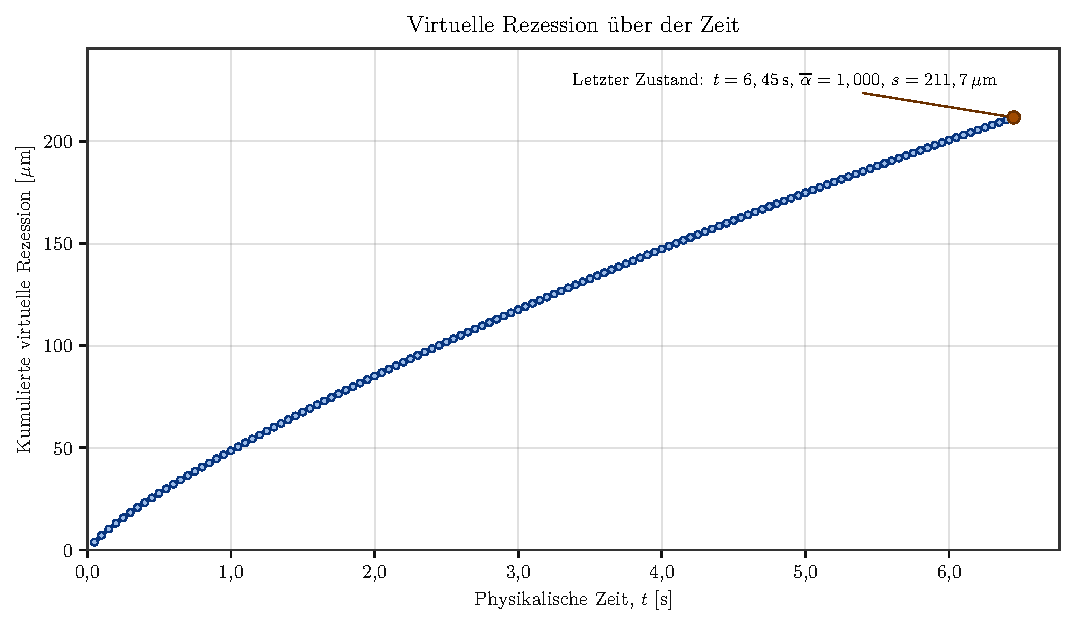
\includegraphics[width=0.96\textwidth]{../analysis/simulation2_recession_vs_time_de.pdf}
\caption{ Akkumulierte virtuelle Rezession versus physische Zeit. Die Kurve wird aus vollständig synchronisierten Zuständen aktualisiert.}
\label{fig:sim2-recession-time}
\end{figure}

\begin{figure}[H]
\centering
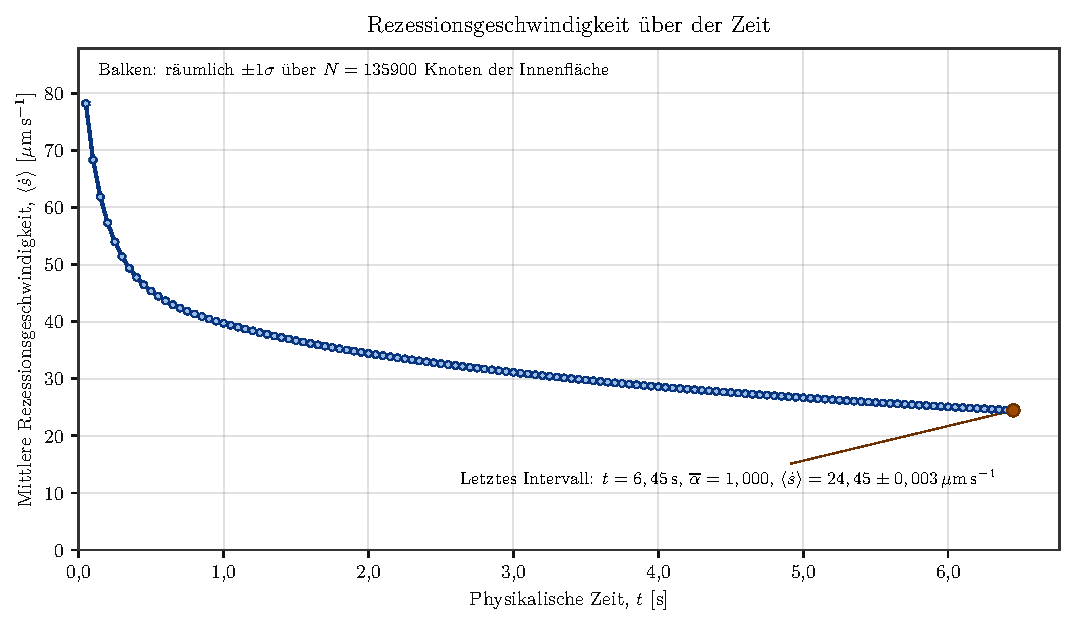
\includegraphics[width=0.96\textwidth]{../analysis/simulation2_recession_rate_vs_time_de.pdf}
\caption{Mittlere Rezessionsrate über die 135\,900 Knoten der Innenfläche. Die Fehlerbalken zeigen die räumliche Streuung \(\pm1\sigma\).}
\label{fig:sim2-rate-time}
\end{figure}

\begin{figure}[H]
\centering
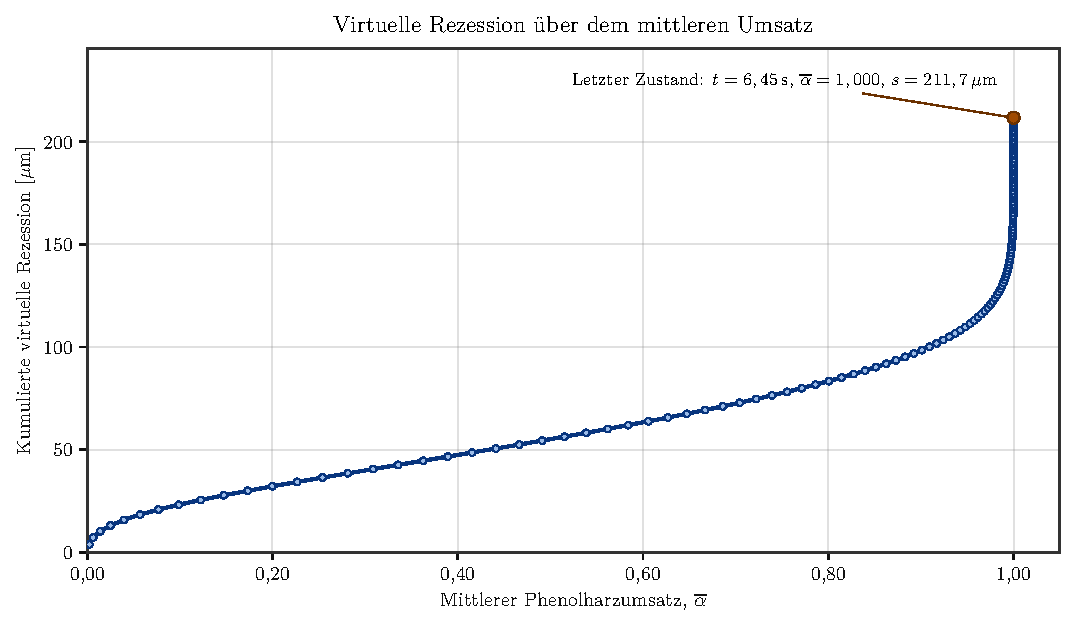
\includegraphics[width=0.96\textwidth]{../analysis/simulation2_recession_vs_alpha_avg_de.pdf}
\caption{Virtual recession versus mean conversion. Die Kurve zeigt, dass die Rezession anhält, nachdem \(\bar\alpha\) fast gesättigt ist.}
\label{fig:sim2-recession-alpha}
\end{figure}

\begin{figure}[H]
\centering
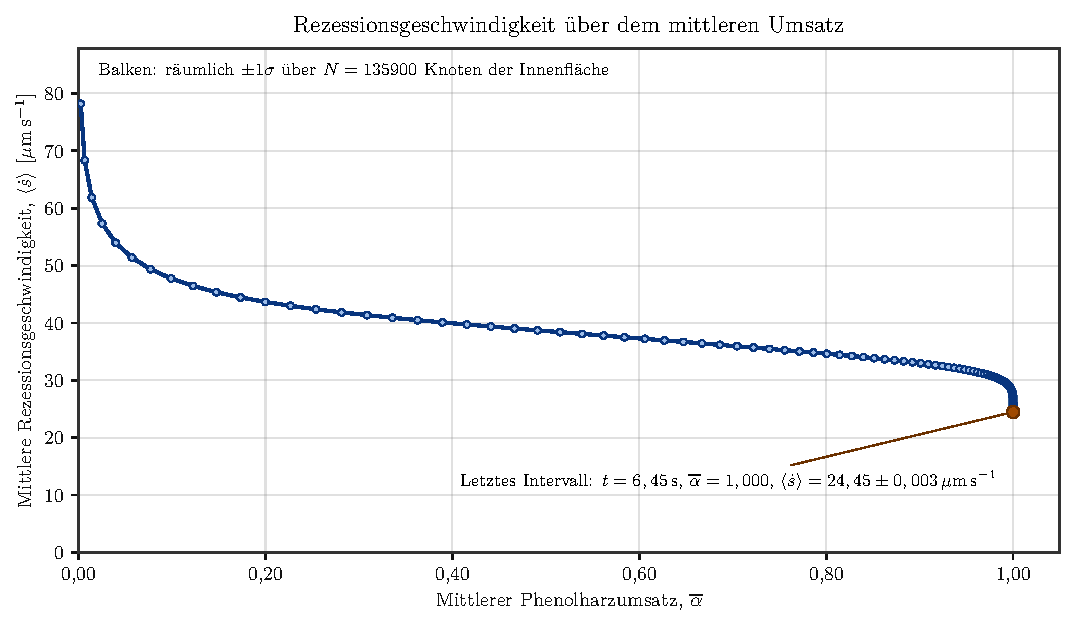
\includegraphics[width=0.96\textwidth]{../analysis/simulation2_recession_rate_vs_alpha_avg_de.pdf}
\caption{Rezessionsrate versus mittlere Umrechnung, mit räumlichem \(\pm1\sigma\).}
\label{fig:sim2-rate-alpha}
\end{figure}

\subsubsection{Räumliche Umwandlung und Pyrolyse-Rate-Profile}

Um einen direkten Vergleich mit Simulation 1 zu ermöglichen, wurden die gleichen fünf Profilfamilien aus den zehn DMP-Partitionen von Simulation 2 rekonstruiert. Die gespeicherten Zustände bei \(t=1,\ldots,6~\si{s}\) sind exakt verfügbar, so dass keine zeitliche Interpolation verwendet wird. Das radiale Gitter liefert jedoch keinen Knoten in jedem der einhundert 1\% Bänder. Bänder ohne Beobachtung sind schraffiert, und nur die aufgetragene Hüllkurve wird linear durch sie interpoliert. Diese Konvention verbessert die visuelle Kontinuität, ohne zusätzliche physikalische Auflösung zu erzeugen.

Die radialen Graphen zeigen auch die vertikale Linie \(d=s(t)\), wobei \(s(t)\) die kumulative Rezession ist, die durch die Energiebilanz des Controllers berechnet wird. Es wurde noch kein Band deaktiviert; die Linie ist daher eine \emph{virtual} Rezessionsposition innerhalb der noch vermaschten ersten Schicht und nicht eine geometrische Grenze, die sich bereits bewegt hat. Sie darf nicht mit einer \(\alpha\) Konversionskontur verwechselt werden.

\begin{figure}[H]
\centering
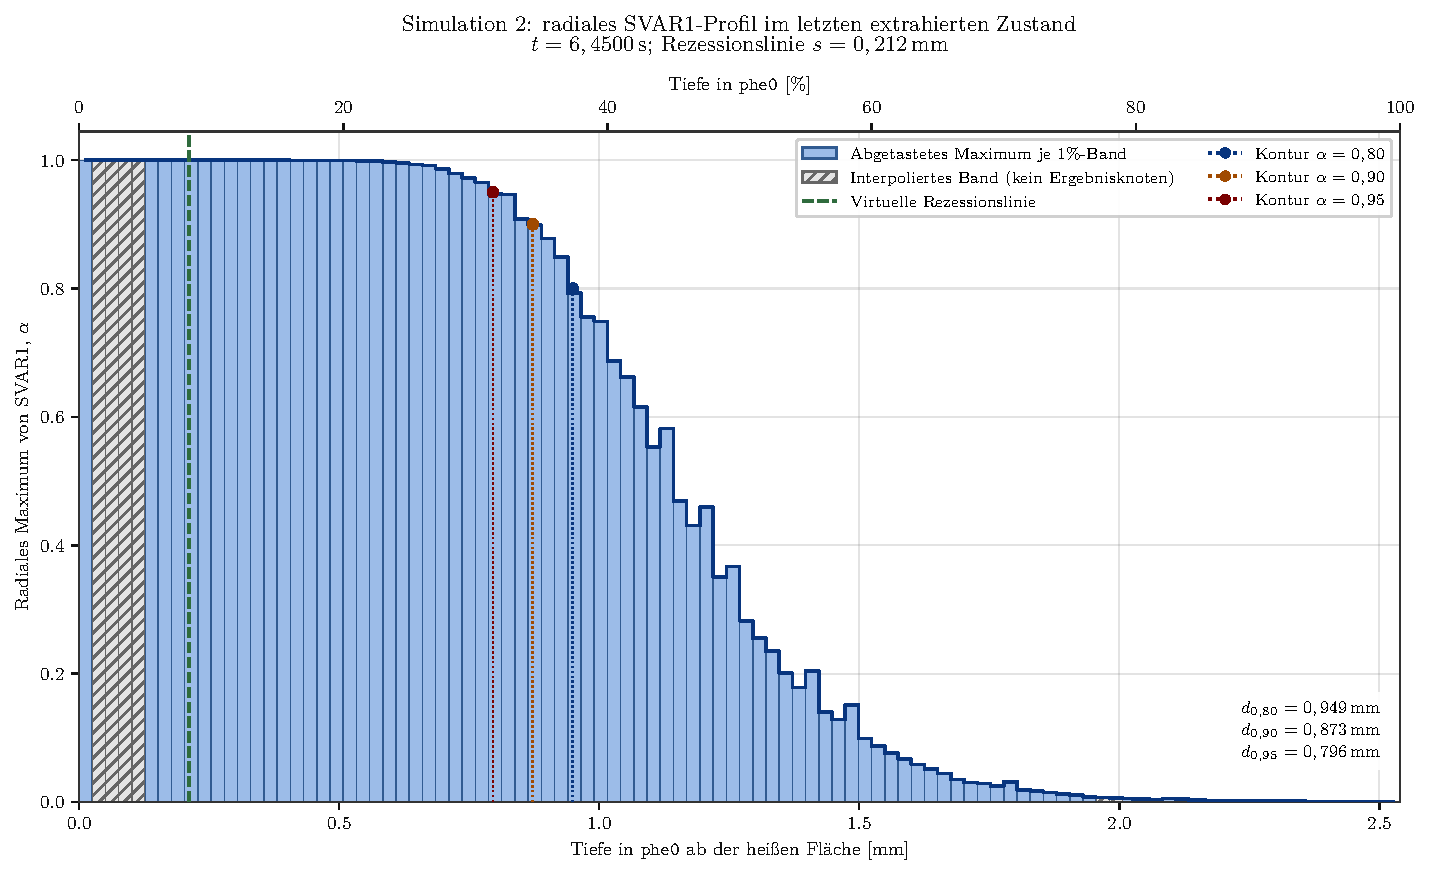
\includegraphics[width=0.98\textwidth]
{../analysis/simulation2_svar1_radial_profile_1pct_de.pdf} \caption{Radiales Maximumprofil von \code{SVAR1} im letzten gemeinsam extrahierten Zustand, einschließlich Umwandlungskonturen und virtueller Rezessionslinie. Schraffierte Bänder enthalten keinen Ergebnisknoten.}
\label{fig:sim2-svar1-radial-de}
\end{figure}

\clearpage
\begin{figure}[H]
\centering
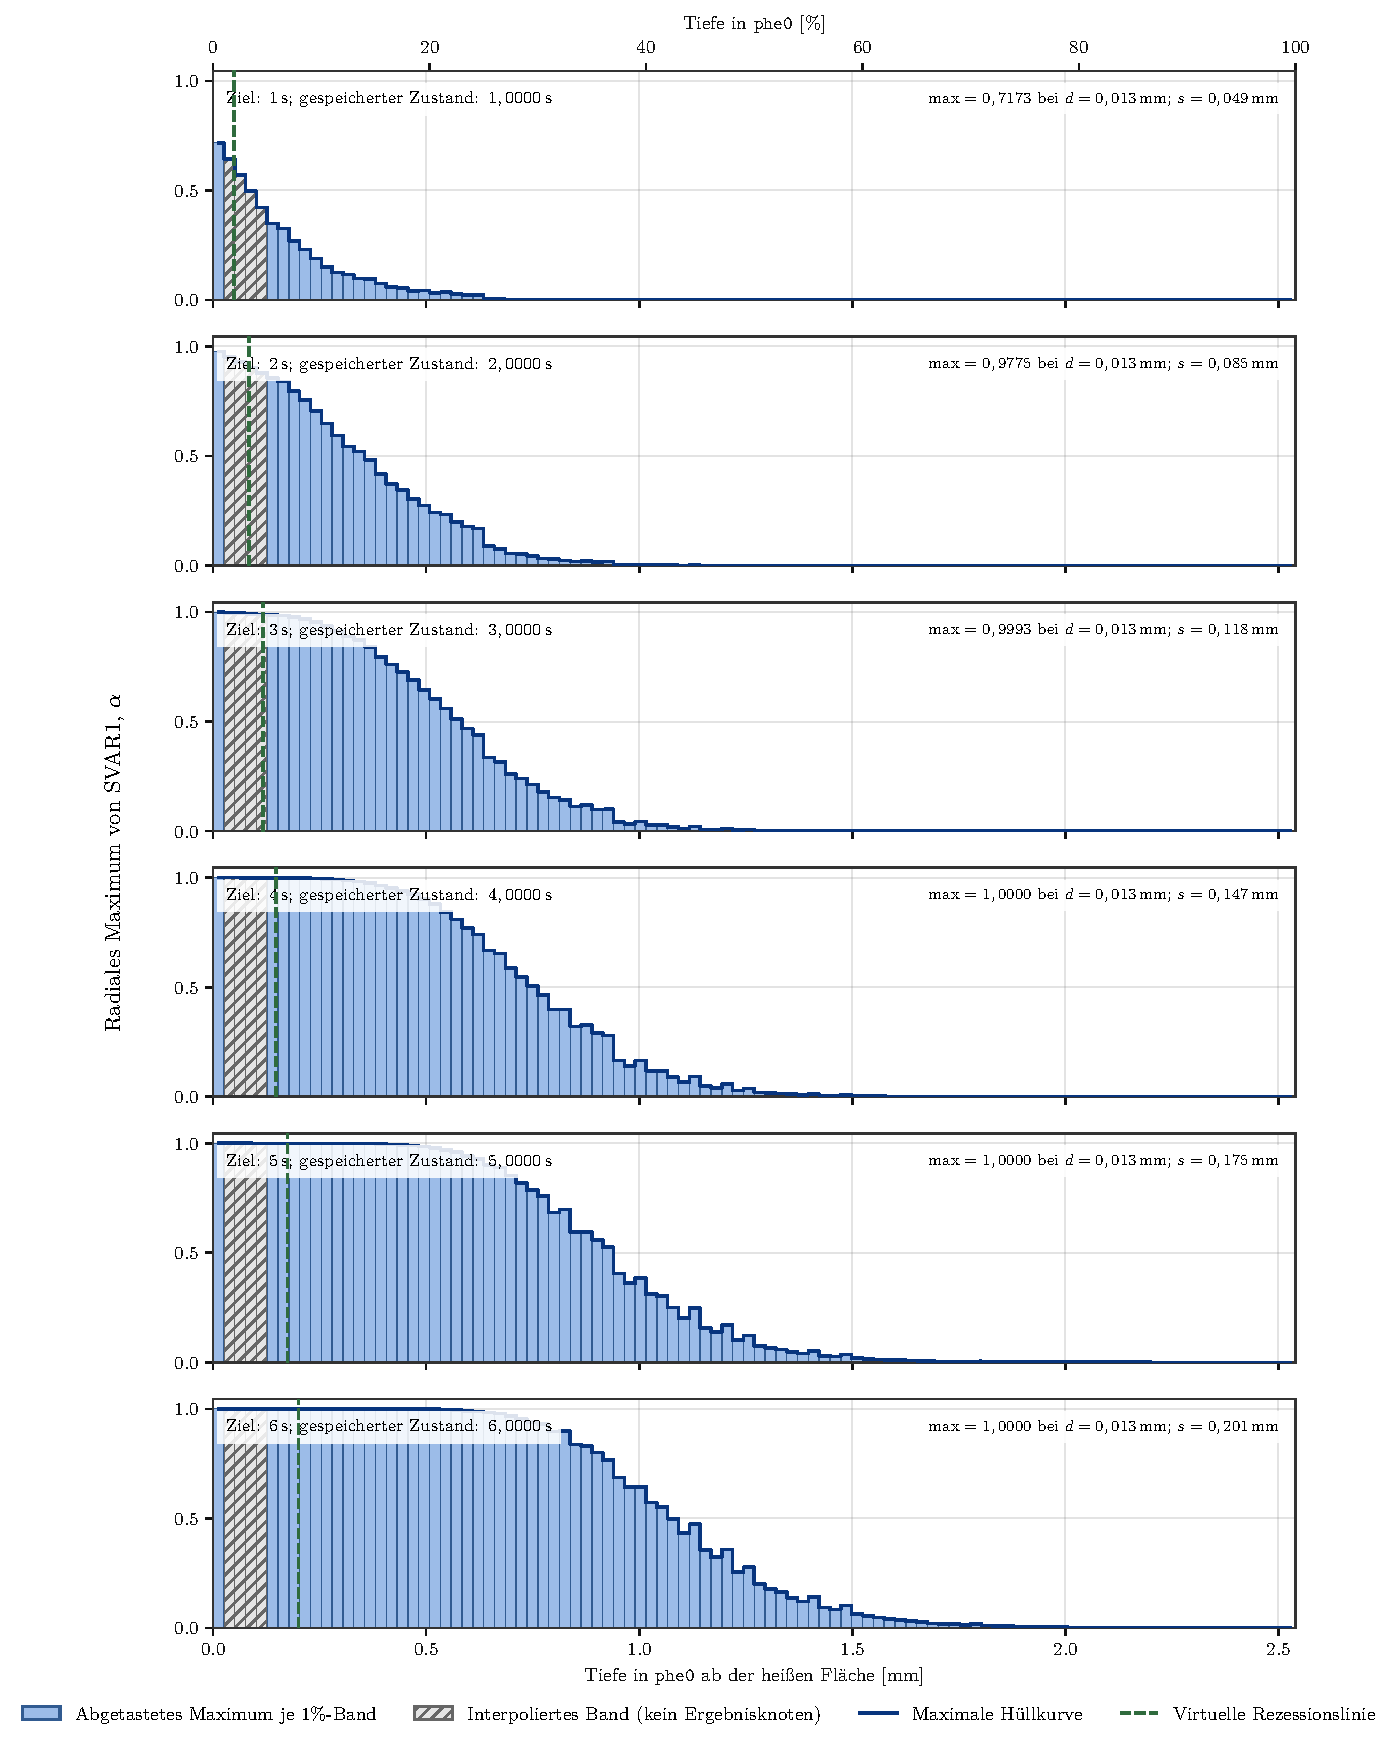
\includegraphics[height=0.80\textheight,width=0.96\textwidth,keepaspectratio]
{../analysis/simulation2_svar1_radial_time_profiles_1pct_de.pdf} \caption{Entwicklung des radialen Maximums von \code{SVAR1} in Simulation 2. Die gestrichelte grüne Linie in jedem Feld markiert die kumulative Position der virtuellen Rezession.}
\label{fig:sim2-svar1-radial-time-de}
\end{figure}

\clearpage
\begin{figure}[H]
\centering
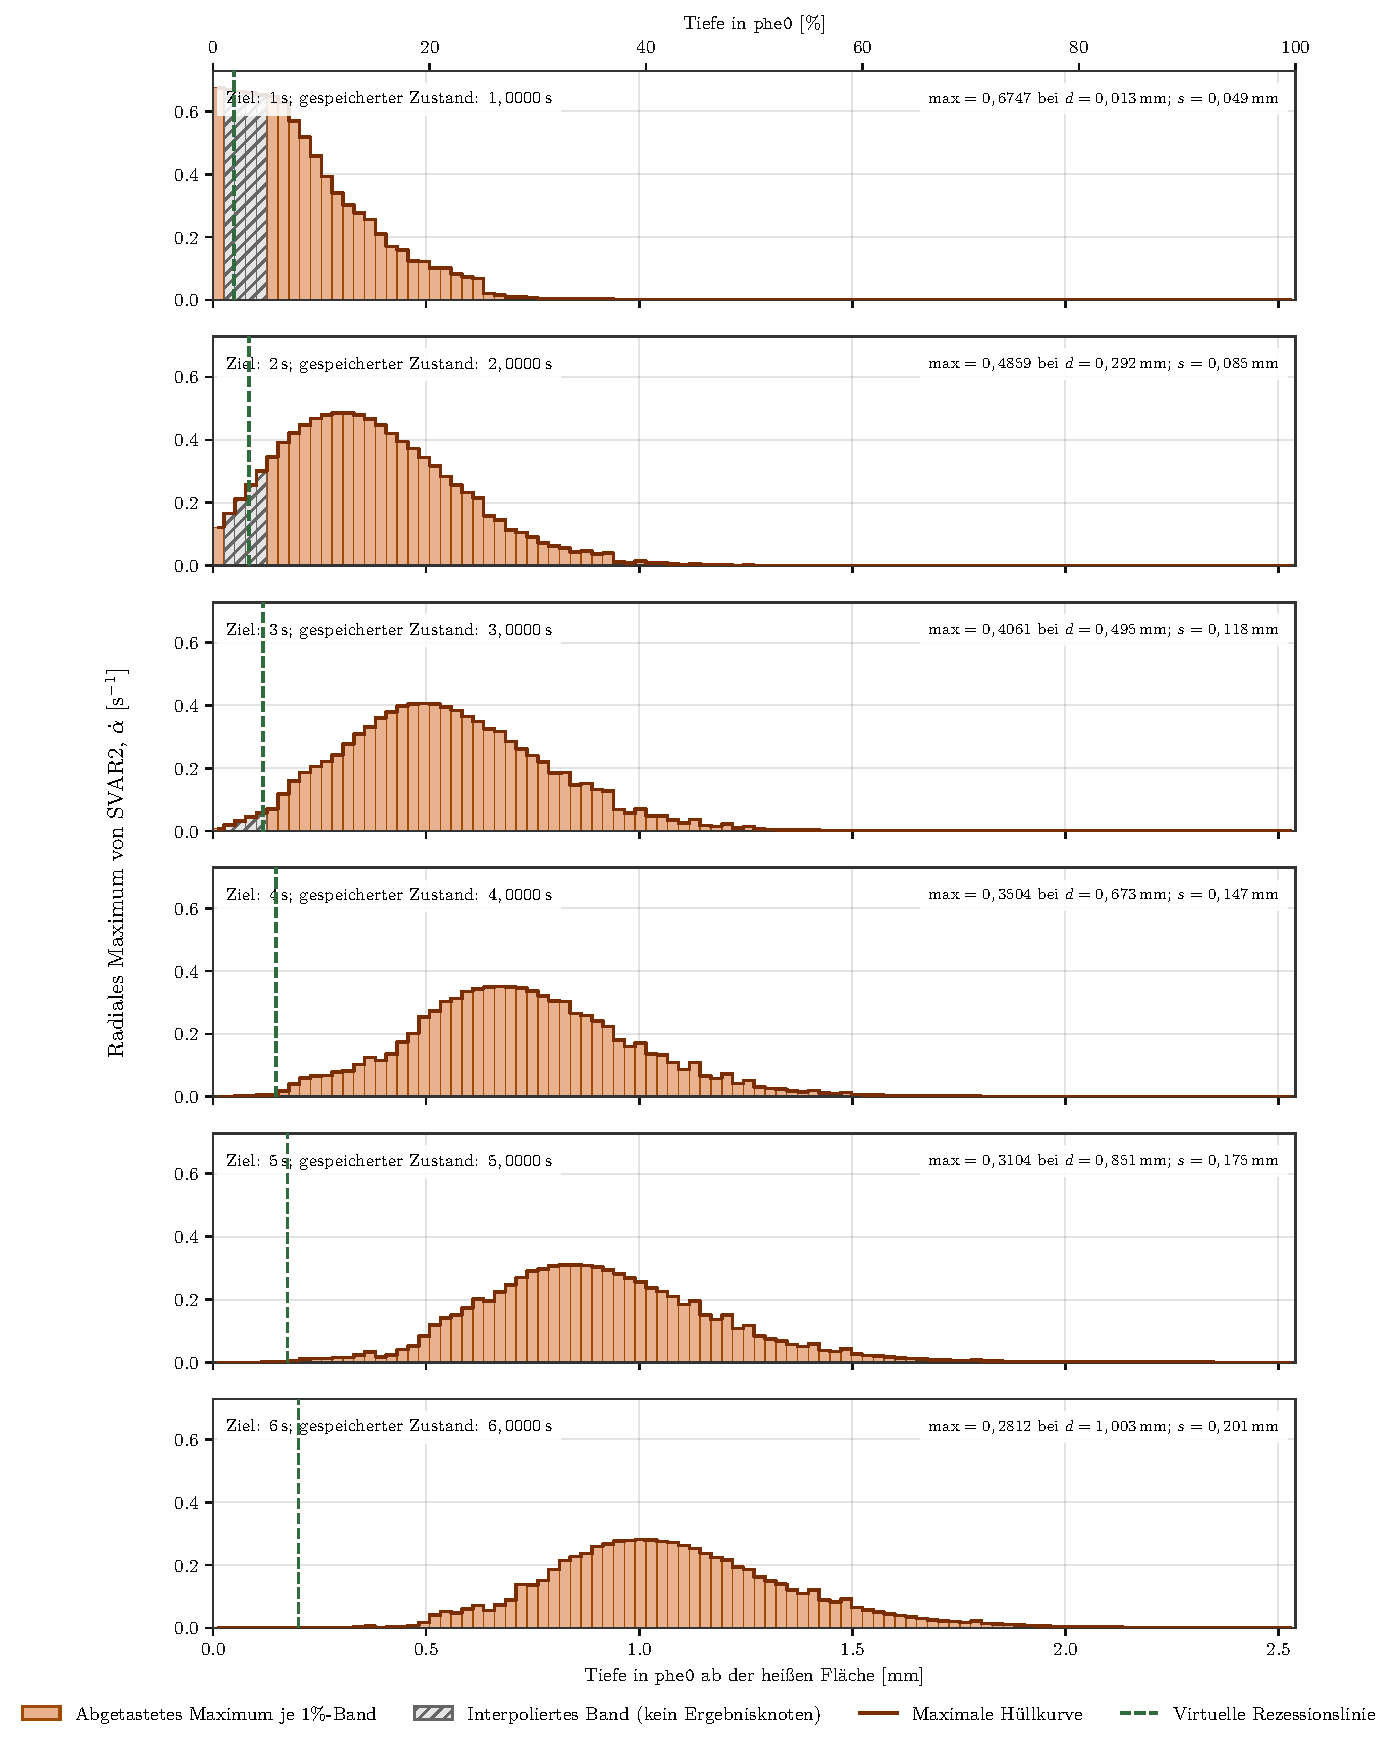
\includegraphics[height=0.80\textheight,width=0.96\textwidth,keepaspectratio]
{../analysis/simulation2_svar2_radial_time_profiles_1pct_de.pdf} \caption{Entwicklung des radialen Maximums von \code{SVAR2}. Die Wanderung der maximalen Pyrolyserate und die Fortschreitung der virtuellen Rezessionslinie werden auf derselben radialen Koordinate dargestellt.}
\label{fig:sim2-svar2-radial-time-de}
\end{figure}

\clearpage
\begin{figure}[H]
\centering
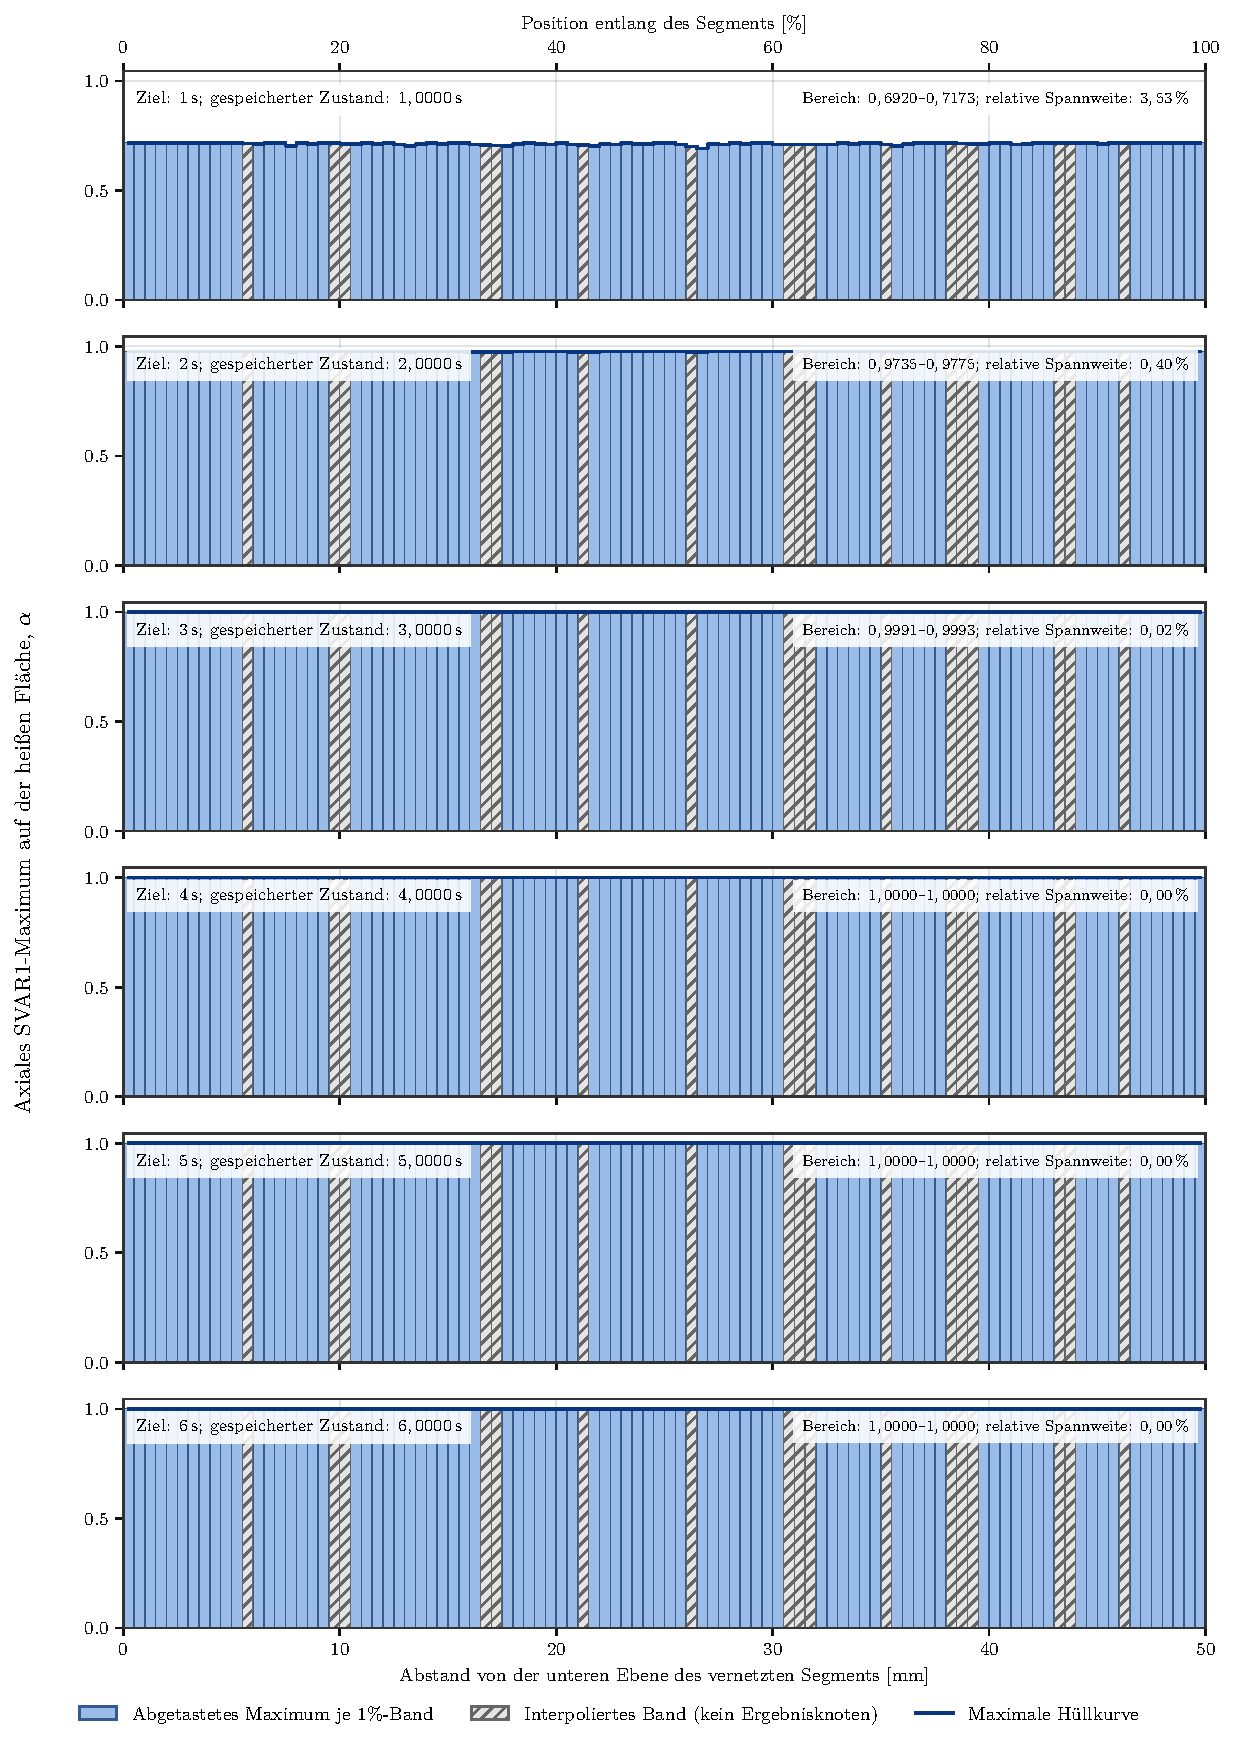
\includegraphics[height=0.80\textheight,width=0.96\textwidth,keepaspectratio]
{../analysis/simulation2_svar1_axial_time_profiles_1pct_de.pdf} \caption{Axiale Abhängigkeit von \code{SVAR1} auf der heißen Innenfläche in Simulation 2. Es wird keine Rezessionslinie eingezeichnet, da die Rezession entlang der radialen Koordinate definiert ist.}
\label{fig:sim2-svar1-axial-time-de}
\end{figure}

\clearpage
\begin{figure}[H]
\centering
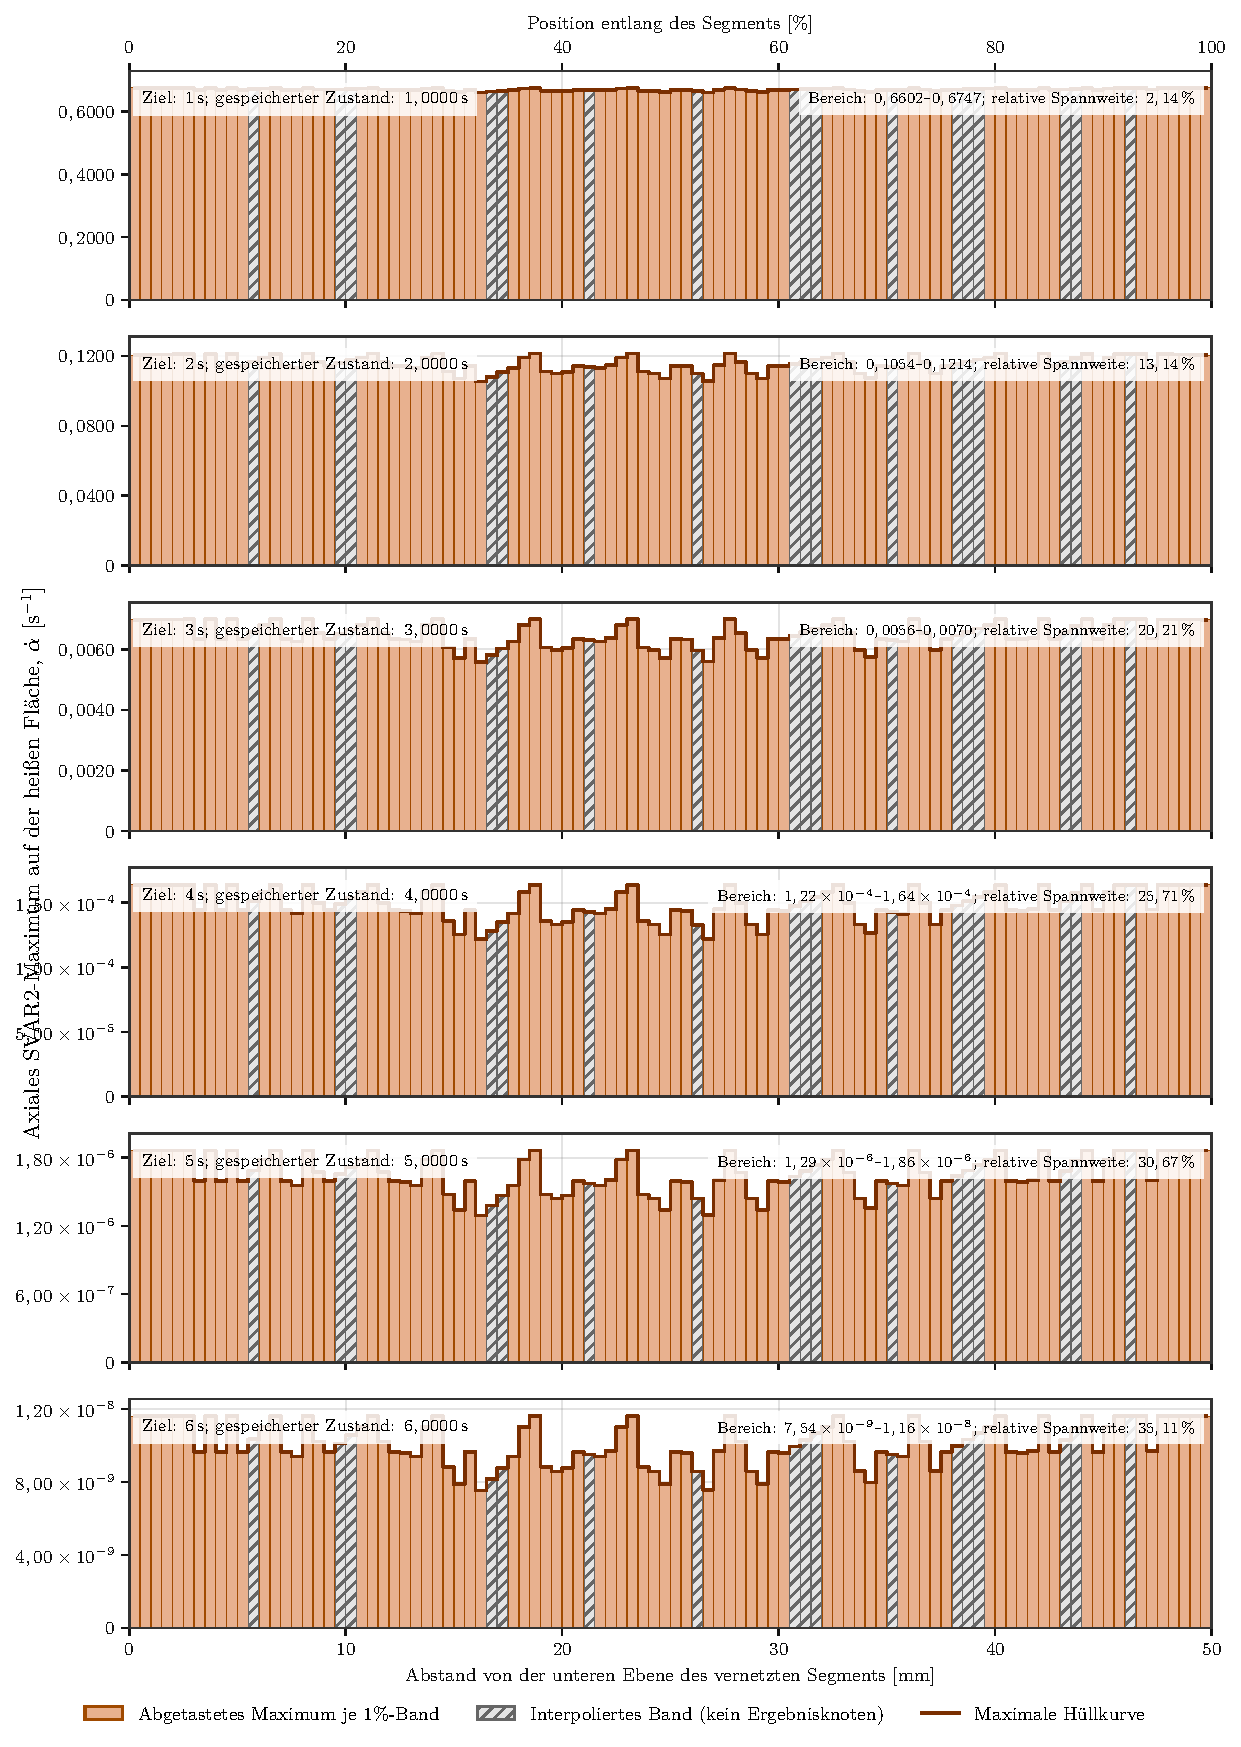
\includegraphics[height=0.80\textheight,width=0.96\textwidth,keepaspectratio]
{../analysis/simulation2_svar2_axial_time_profiles_1pct_de.pdf} \caption{Axiale Abhängigkeit von \code{SVAR2} auf der heißen Innenfläche in Simulation 2. Eine unabhängige vertikale Skala in jedem Feld macht die kleinen Werte nach der Oberflächensättigung sichtbar.}
\label{fig:sim2-svar2-axial-time-de}
\end{figure}
\clearpage

Die Daten behalten 16 radiale Bänder und 17 axiale Bänder ohne Ergebnisknoten, die alle explizit durch Schraffur markiert sind. Bei \SI{1}{s} ist die maximale radiale Umwandlung \(\alpha_\mathrm{max}=0.7173\); sie erreicht numerische Einheit bei \SI{6}{s}. Gleichzeitig sinkt die maximale Pyrolyserate von \SI{0.6747}{s^{-1}} auf \SI{0.2812}{s^{-1}} und wandert von \SI{0.0127}{mm} auf \SI{1.0033}{mm} vom heißen Gesicht ab. Im letzten extrahierten Zustand \SI{6.45}{s} ist es \SI{0.2703}{s^{-1}} bei \SI{1.0795}{mm}.

Die Rezessionslinie verläuft von \SI{0.0486}{mm} bei \SI{1}{s} zu \SI{0.2006}{mm} bei \SI{6}{s} und dann zu \SI{0.2044}{mm} bei \SI{6.15}{s} und \SI{0.2117}{mm} bei \SI{6.45}{s}. Ab \SI{2}{s} bleibt sie weit vor dem maximalen SVAR 2. Die Figuren unterscheiden somit visuell zwei verschiedene Mechanismen: die volumetrische Zone, in der die Pyrolyse am aktivsten ist, und die kumulative Materialposition, die die Energiebilanz zurücknehmen würde. Auf der heißen Oberfläche wird SVAR1 bei Einheit axial einheitlich. Späte relative Schwankungen von SVAR2 erreichen ungefähr 35\%, aber nur für absolute Werte der Ordnung \(10^{-8}~\si{s^{-1}}\) und sind daher physikalisch vernachlässigbar.

\clearpage
\begin{figure}[H]
\centering
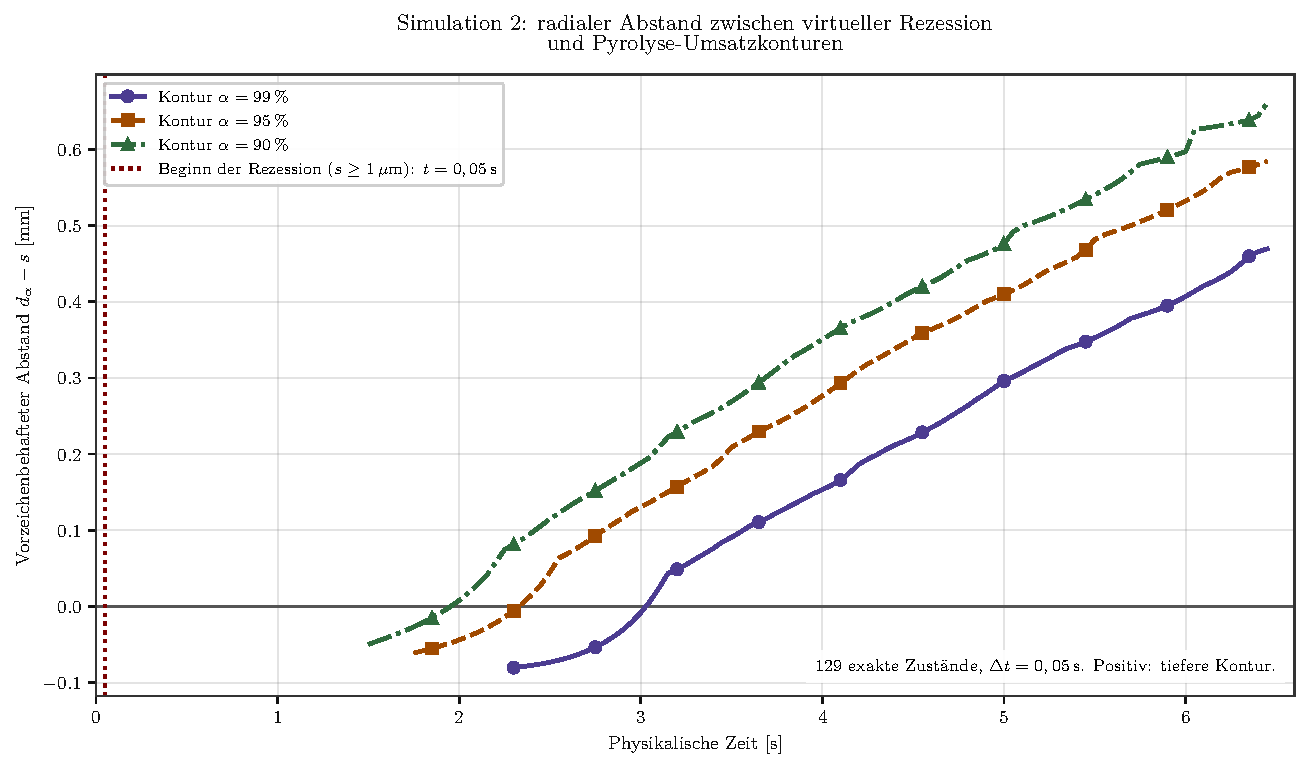
\includegraphics[width=0.94\textwidth]
{../analysis/simulation2_recession_to_pyrolysis_contours_vs_time_de.pdf} \caption{Signierter radialer Abstand zwischen der virtuellen Rezessionslinie und den Pyrolyse-Umwandlungskonturen bei 99\%, 95\% und 90\%. Der Abstand ist als \(\Delta d_\alpha=d_\alpha-s\) definiert: Ein positiver Wert ordnet die Kontur tiefer in der Wand als die Rezession ein. Die vertikale gestrichelte Linie markiert den ersten Zustand, in dem die virtuelle Rezession \SI{1}{\micro m} erreicht.}
\label{fig:sim2-recession-contour-distance-de}
\end{figure}

Die Konturen ergeben sich durch räumliche Interpolation der radialen \code{SVAR1} Hüllkurve überhaupt 129 synchronisierten Zustände, beabstandet durch \SI{0.05}{s} von \SI{0.05}{s} bis \SI{6.45}{s}; es wird keine zeitliche Interpolation eingeführt. Die vertikale Linie bei \SI{0.05}{s} identifiziert den ersten Zustand, für den \(s\geq\SI{1}{\micro m}\), mit \(s=\SI{3.802}{\micro m}\). Mit diesem Mikrometer-Schwellenwert wird vermieden, dass abgerundete Rückstände als Front-Onset behandelt werden, während sie weit unter der radialen Auflösung des Modells bleiben. Eine Kurve beginnt erst, wenn ihre Umwandlungsschwelle tatsächlich erreicht ist, so dass fehlende Beobachtungen nicht durch künstliche Nullen ersetzt werden. Die Konturen von 90\%, 95\% und 99\% erscheinen zuerst bei \SI{1.50}{s}, \SI{1.75}{s} und \SI{2.30}{s}, jeweils zunächst vor der Rezession mit \(\Delta d_\alpha=\SI{-0.0497}{mm}\), \SI{-0.0611}{mm} und \SI{-0.0803}{mm}. Sie passieren dann die Rezessionslinie bei \SI{2.00}{s}, \SI{2.35}{s} und \SI{3.05}{s}. Spätestens im extrahierten Zustand \SI{6.45}{s} erreichen die Trennungen \SI{0.4693}{mm}, \SI{0.5843}{mm} und \SI{0.6610}{mm} für die Konturen 99\%, 95\% bzw. 90\%. Das Wachstum aller drei Trennungen zeigt, dass die Umwandlungsfront schneller durch die Dicke vorrückt als die virtuelle Rezession.

\subsubsection{Kampagnenabschluss und verbleibende Arbeit}

Das Hauptergebnis der Kampagne ist zweifach. Erstens hat die \code{UserMatTh}--outgassing--blowing--recession--distributed-restart-Kette über 129 synchronisierte Makroschritte ohne Verlust der Kontinuität funktioniert. Zweitens bleibt die Rezession mit \(H_\mathrm{eff}=\SI{35}{MJ.kg^{-1}}\) unter einem Band bei \SI{6.45}{s}; der Pilot hat daher keine diskrete Bewegung der heißen Grenze vor dem absichtlichen Stopp vorhergesagt. Konversion Fortschritte tiefer als virtuelle Rezession, während outgassing und Blasen Rückgang nach ihrem Höhepunkt.

Diese Schlussfolgerung ist streng auf das berechnete \SIrange{0}{6.45}{s} Intervall beschränkt. Es wird nicht bestimmt, ob das erste Band während des nicht berechneten \SI{0.55}{s} gekreuzt würde. Noch wichtiger ist, dass die ausgeführte Geometrie Nenndurchmesser als Radien verwendet, so dass die quantitativen Werte den Nennmotor nicht beschreiben. Vor der Qualifizierung muss die Geometrie korrigiert und die Analyse wiederholt werden; Massen- und Energiebilanzen müssen geschlossen werden; PCG und SPARSE müssen verglichen werden; Mesh-Konvergenz mit 20 zu 40 Radialbänder müssen nachgewiesen werden; Empfindlichkeit gegenüber \(H_\mathrm{eff}\), \(h_0\), der Zeitschritt und die Char-Eigenschaften müssen bewertet werden; und das Modell muss mit einem instrumentierten Test verglichen werden. Ohne diese Schritte bleibt die berechnete Rezession ein Modell-Leistungsindikator, keine qualifizierte motorische Vorhersage.

% ============================================================================
\clearpage
\section{Simulation 3: Korrigierter Dünnsektor mit verfeinertem Radialnetz}

\subsection{Ziel und ausgeführte Konfiguration}

Simulation 3 überträgt die Simulation 2 thermochemische Kette auf eine korrigierte Geometrie, die in Umfangsrichtung stark reduziert ist. Das Modell stellt einen Sektor \(0.10^\circ\) mit einer axialen Länge von \SI{50}{mm} dar. Es behält die vier koaxialen Schichten an ihren tatsächlichen Radien: \code{phe0} von \SIrange{66.675}{67.945}{mm}, Epoxy von \SIrange{67.945}{68.2625}{mm}, \code{phe1} von \SIrange{68.2625}{71.4375}{mm} und Aluminium von \SIrange{71.4375}{76.2}{mm}. Ein voller Ring enthält 3,600 solche Sektoren; nur umfangreiche Mengen werden mit diesem Faktor multipliziert. Temperaturen, Umwandlungen, Oberflächenflüsse und Rezessionstiefen werden nicht neu skaliert.

Der Sektor ist diskretisiert mit 35,200 linearen Achtknoten-Hexaedern und 54,540 Knoten. Das Netz enthält 100 axiale Teilungen, zwei umlaufende Teilungen und 64, 16, 64 und 32 radiale Teilungen in \code{phe0}, Epoxy, \code{phe1} und Aluminium. Die Soll-Radialsteigung der ersten Schicht ist daher
\[
  \Delta r_\mathrm{phe0}=\frac{\SI{1.27}{mm}}{64}
  =\SI{19.84375}{\micro m},
\]
Das ist sechzehnmal feiner als die in der Simulation verwendeten \SI{317.5}{\micro m} Bänder. Drei verklebte Grenzflächen sorgen für thermische Kontinuität zwischen den vier Körpern.

Die nichtlineare transiente thermische Lösung wurde in Mechanical/MAPDL 2026 R1.02 auf zehn DMP-Rängen ausgeführt. Sein Horizont bleibt \SI{7}{s}, unterteilt in 140 Makroschritte von \SI{0.05}{s}. Der Controller fügt nach jedem konvergierten Makroschritt eine Historienzeile hinzu und behält vier Neustartgenerationen bei. Dieses Design unterstützt einen kontrollierten Stopp, ohne bereits konvergierte Zustände zu verlieren.

\begin{table}[H]
\centering
\small
\renewcommand{\arraystretch}{1.15}
\begin{tabular}{L{0.43\textwidth}L{0.43\textwidth}}
\toprule
\textbf{Parameter} & \textbf{Durchgeführte Simulation 3 Wert} \\
\midrule
Sektor und Länge & \(0.10^\circ\); \SI{50}{mm} \\
Heißer / äußerer Radius & \SI{66.675}{mm} / \SI{76.2}{mm} \\
Netz & 54\,540 Knoten; 35\,200 lineare Hexaeder \\
\(z/\theta\) Divisionen & 100 / 2 \\
Radiale Divisionen & 64 / 16 / 64 / 32 \\
Radiale Steigung in \code{phe0} & \SI{19.84375}{\micro m} \\
Kontakte & 3 gebundene Schnittstellen \\
Parallele Ausführung & 10 DMP-Ranks \\
Zeithorizont & \SI{7}{s}; 140 Schritte von \SI{0.05}{s} \\
Vollring-Skalafaktor & 3,600, nur für umfangreiche Mengen \\
\bottomrule
\end{tabular}
\caption{Geometrie und Netz der ausgeführten Simulation 3.}
\label{tab:sim3-configuration}
\end{table}

\subsection{Endstatus und Rechenleistung}

Der Lauf wurde am 18. September 2026 regulär abgeschlossen. Alle 140 Makroschritte konvergierten bis \(t=\SI{7.00}{s}\). Die 140 Historienzeilen sind gleichmäßig in Abständen von \SI{0.05}{s} angeordnet; Zeitpunkte fehlen nicht und treten nicht doppelt auf. MAPDL meldet ausdrücklich \code{RUN COMPLETED}; nach Abschluss verblieb kein Prozess \code{ANSYS.exe}, \code{mpiexec.exe} oder \code{hydra\_pmi\_proxy.exe}.

Die gesamte verstrichene Zeit ist \SI{5188.519}{s}, oder 86 min 28.5 s, entsprechend einem Durchschnitt von 37.1 s pro Makroschritt. Die Lösungsberechnung berücksichtigt \SI{984.3}{s} (19.0\%), während die Lösungsnachbearbeitung \SI{3765.9}{s} (72.6\%) berücksichtigt. Diese Verteilung zeigt, dass das Schreiben und Zusammensetzen von Ergebnissen die Kosten des Dünnsektorlaufs dominiert. Die zehn Ränge schrieben \SI{396.2}{GB} und lasen \SI{82.5}{GB}; Arbeitsdateien belegen \SI{7656.1}{MB}. Die Gesamtspeichernutzung erreichte \SI{828}{MB}, wobei \SI{4032}{MB} zugewiesen wurde.

Das Protokoll enthält keinen Fehler und zwölf Warnungen. Sie betreffen die deaktivierte Elementformprüfung, die Standard-Implementierung \code{USERCK}, die Auswertung bei \SI{22}{\celsius} unterhalb der ersten tabellarisierten Temperatur mehrerer Materialeigenschaften und einen ignorierten Befehl \code{CEWRITE} nach dem Lösen. Keine dieser Nachrichten verhinderte die Konvergenz, die Produktion aller zehn RTH-Partitionen oder die Aufzeichnung der Zustände 140.

\begin{table}[H]
\centering
\small
\renewcommand{\arraystretch}{1.15}
\begin{tabular}{L{0.49\textwidth}L{0.37\textwidth}}
\toprule
\textbf{Kenngröße} & \textbf{Endwert} \\
\midrule
Konvergierte Zustände & 140 von 140; \SIrange{0.05}{7.00}{s} \\
Parallele Ausführung & 10 DMP-Ranks, spärlicher Direktlöser \\
Verstrichene / aggregierte CPU-Zeit & \SI{5188.519}{s} / \SI{5882.922}{s} \\
Lösungsberechnungszeit & \SI{984.3}{s} \\
Nachbearbeitungszeit der Lösung & \SI{3765.9}{s} \\
Disk I/O gelesen / geschrieben & \SI{82.5}{GB} / \SI{396.2}{GB} \\
Fehler / Warnungen & 0 / 12 \\
MAPDL Ergebnis & \code{RUN COMPLETED} \\
\bottomrule
\end{tabular}
\caption{Endsimulation 3 Leistungszusammenfassung.}
\label{tab:sim3-performance}
\end{table}

\subsection{Endgültige thermochemische Ergebnisse}

Die erste aktive Zeile kreuzt den Schwellenwert \(\alpha=0.99\) bei \SI{2.60}{s}, mit \(\alpha=0.99050948\); der Controller deaktiviert dann 200 \code{phe0} Hexaeder. Die zweite Zeile kreuzt den gleichen Schwellenwert bei \SI{2.95}{s}, mit \(\alpha=0.99021488\), und eine weitere 200 Hexaeder werden deaktiviert. Insgesamt werden 400 phenolische Elemente gelöscht und kein Epoxy, \code{phe1} oder Aluminiumelement entfernt. Der diskrete Heißradius bewegt sich von \SI{66.675}{mm} zu \SI{66.714688}{mm} oder zwei radialen Steigungen. Die dritte Zeile bleibt aktiv: Ihre Umwandlung ist 0.98643222 bei \SI{3.00}{s} und 0.98962501 bei \SI{7.00}{s}, knapp unterhalb des Löschkriteriums. Die Gleichheit der Mittelwerte und der Mindestwerte für die Historie steht im Einklang mit der Sektorsymmetrie und wird im Folgenden durch die räumliche DPF-Extraktion überprüft.

Der Wandgasmassenfluss erreicht einen Spitzenwert bei \SI{0.1220}{kg.m^{-2}.s^{-1}} bei \SI{1.80}{s} und fällt dann bei \SI{0.001636}{kg.m^{-2}.s^{-1}} bei \SI{7.00}{s} ab. Sektorstromspitzen bei \SI{0.7099}{mg.s^{-1}} und enden bei \SI{0.009522}{mg.s^{-1}}. Sein Zeitintegral ist \SI{1.689}{mg} für den Sektor oder \SI{6.080}{g} für den kompletten Ring durch den einfachen Faktor 3,600. Der effektive Konvektionskoeffizient erreicht ein Minimum von \SI{836.67}{W.m^{-2}.K^{-1}} bei Spitzenausgasung und erholt sich zu \SI{997.39}{W.m^{-2}.K^{-1}}. Maximale Temperaturspitzen bei \SI{1400.50}{\celsius} bei \SI{2.60}{s}, fallen dann bei Fertigstellung auf \SI{435.36}{\celsius}, wenn innere Reihen freigelegt werden.

\begin{figure}[H]
\centering
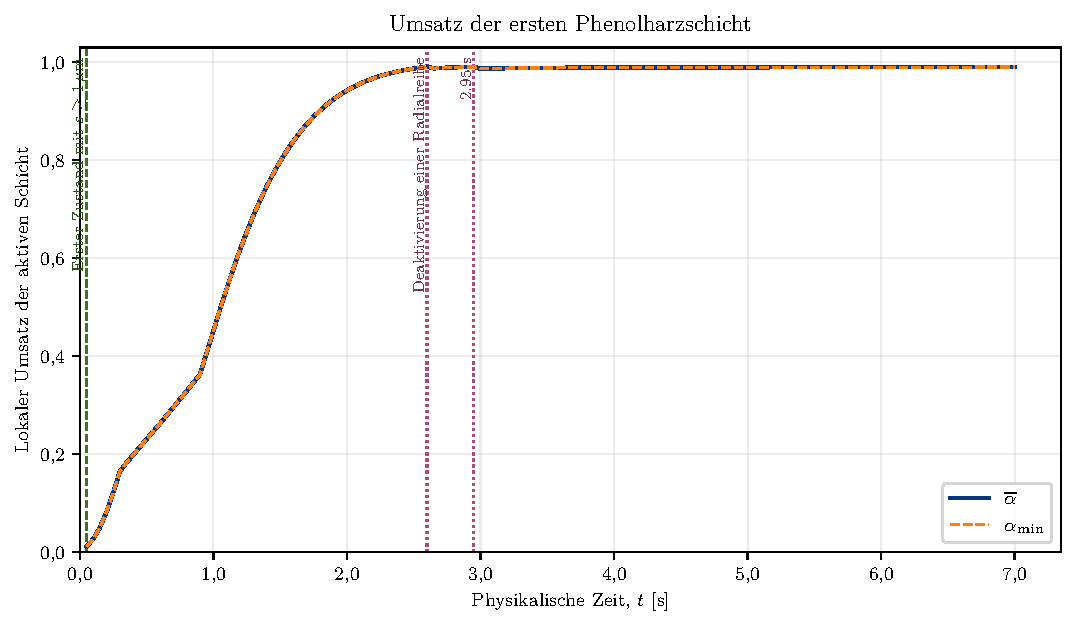
\includegraphics[width=0.96\textwidth]{../analysis/simulation3_sector_conversion_vs_time_de.pdf}
\caption{In der aktiven Schicht des dünnen Sektors über alle konvergierten Zustände 140 aufgezeichnete mittlere und minimale Umwandlung. Vertikale Linien markieren die beiden radialreihigen Deaktivierungen.}
\label{fig:sim3-conversion-time-de}
\end{figure}

\begin{figure}[H]
\centering
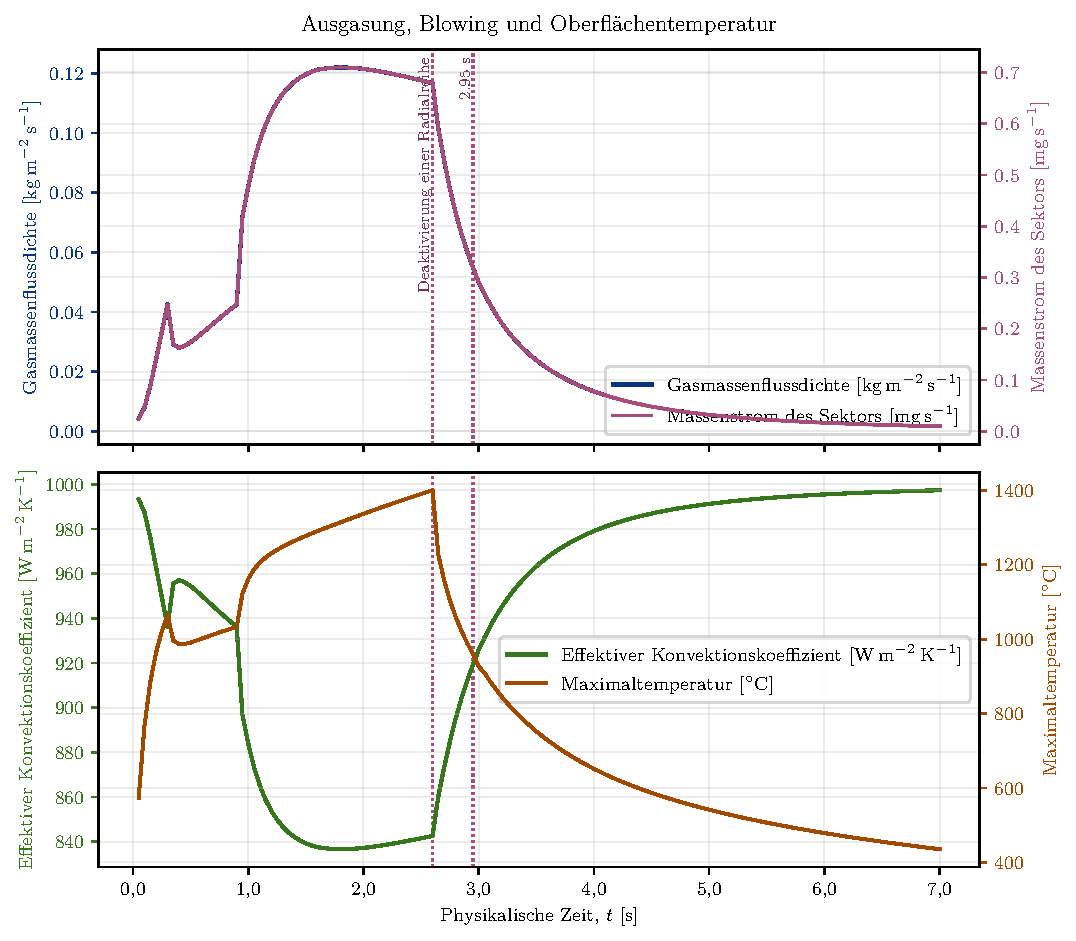
\includegraphics[width=0.96\textwidth]{../analysis/simulation3_sector_thermal_gas_overview_de.pdf}
\caption{ Entwicklung der Ausgasung, des effektiven Konvektionskoeffizienten und der maximalen Temperatur der heißen Oberfläche. Der Gesamtfluss gilt für den Sektor \(0.10^\circ\).}
\label{fig:sim3-thermal-gas-de}
\end{figure}

\subsection{Virtuelle Rezession und Elementdeaktivierung}

Die kumulierte energiebasierte Rezession erreicht \SI{446.254}{\micro m} bei \SI{7.00}{s}. Die diskrete Oberfläche hat sich nur um \SI{39.6875}{\micro m} bewegt, da das Löschen sowohl den geometrischen Schwellenwert als auch \(\alpha\geq0.99\) erfordert. Virtuelle Rezession überschreitet daher die dritte Reihenschwelle von \SI{59.53125}{\micro m}, aber die endgültige Umwandlung dieser Zeile bleibt bei 0.98962501, so dass der Controller sie korrekt aktiv hält. Der Endzustand bestätigt \code{SIM2\_ILAY=2} und \code{SIM2\_NEL=200}. Die schmalen ganzzahligen Felder der Geschichte zeigen \code{****} und \code{**} an; die Plots ignorieren nur diese beiden unlesbaren Felder und behalten jede gültige physikalische Spalte bei.

Numerisch signifikanter Rezessionsbeginn ist definiert als \(s\ge\SI{1}{\micro m}\). Es tritt im ersten aufgezeichneten Makroschritt bei \SI{0.05}{s} auf, wobei \(s=\SI{3.918}{\micro m}\). Die Zeitdiagramme markieren diesen Zeitpunkt mit einer vertikalen Linie; zwei gestrichelte Linien markieren Deaktivierungen bei \SI{2.60}{s} und \SI{2.95}{s}. Die unten gezeigte Rate ist die endliche Differenz der akkumulierten Rezession zwischen aufeinanderfolgenden Makroschritten; sie ist \SI{78.37}{\micro m.s^{-1}} im ersten Intervall und \SI{85.28}{\micro m.s^{-1}} im letzten Intervall. Plots gegen \(\overline{\alpha}\) bewahren die Diskontinuitäten, die durch das Umschalten von einer aktiven Zeile zur nächsten verursacht werden.

\begin{figure}[H]
\centering
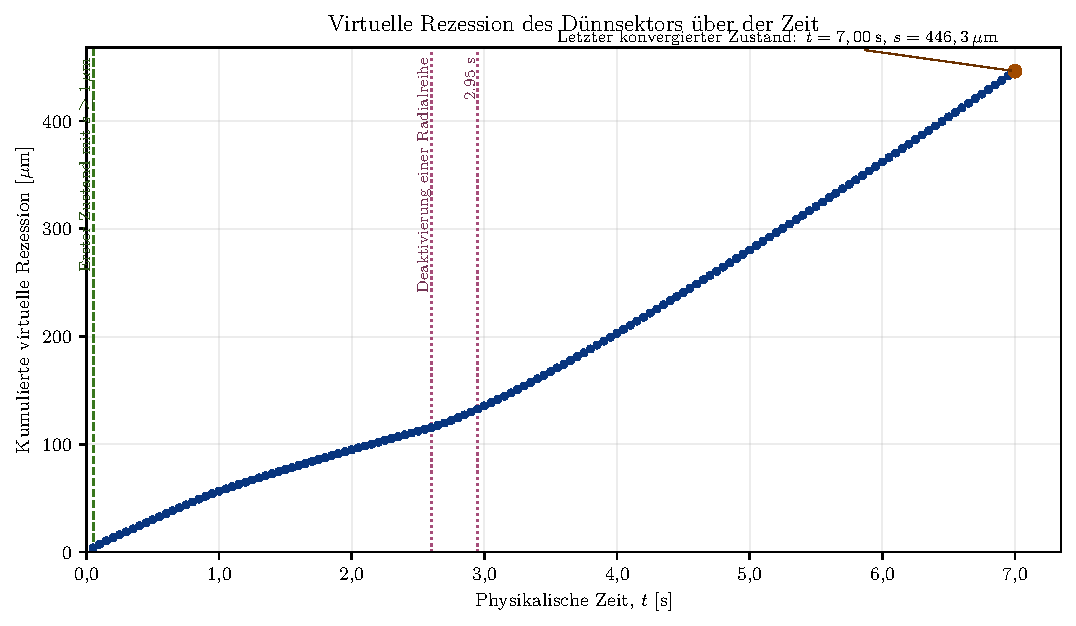
\includegraphics[width=0.96\textwidth]{../analysis/simulation3_sector_recession_vs_time_de.pdf}
\caption{Akkumulierte virtuelle Rezession gegen Zeit für Simulation 3. Die vertikalen Linien markieren den numerischen Beginn der Rezessionsfront und beide radialreihige Deaktivierungen.}
\label{fig:sim3-recession-time-de}
\end{figure}

\begin{figure}[H]
\centering
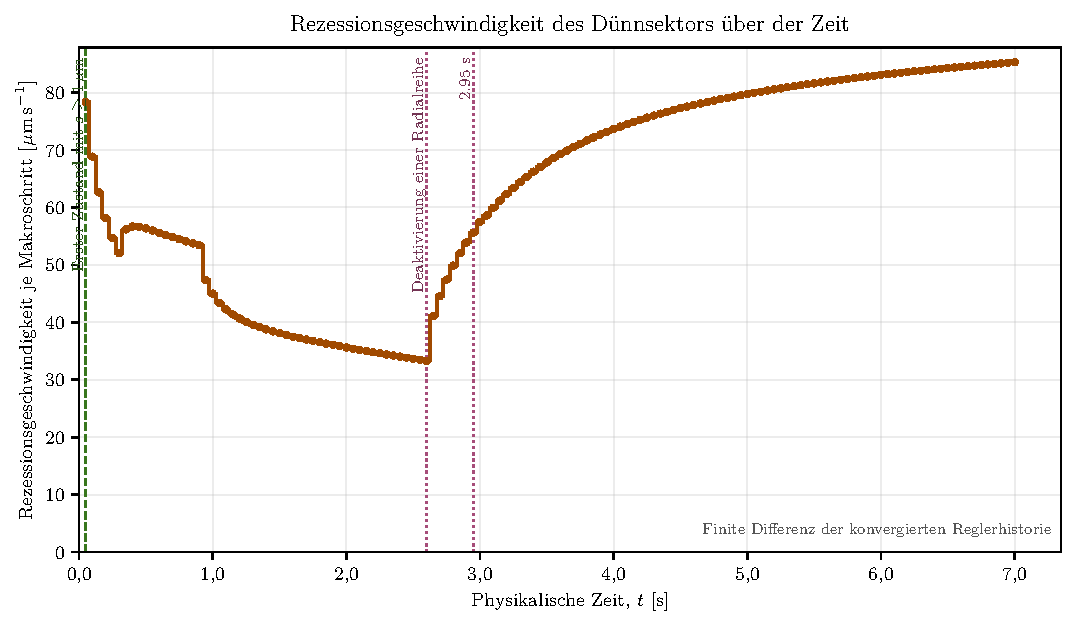
\includegraphics[width=0.96\textwidth]{../analysis/simulation3_sector_recession_rate_vs_time_de.pdf}
\caption{Makroschritt-Rezessionsrate. Dies ist eine zeitliche Ableitung der Controller-Historie, ohne einen räumlichen Standardabweichungsbalken.}
\label{fig:sim3-rate-time-de}
\end{figure}

\begin{figure}[H]
\centering
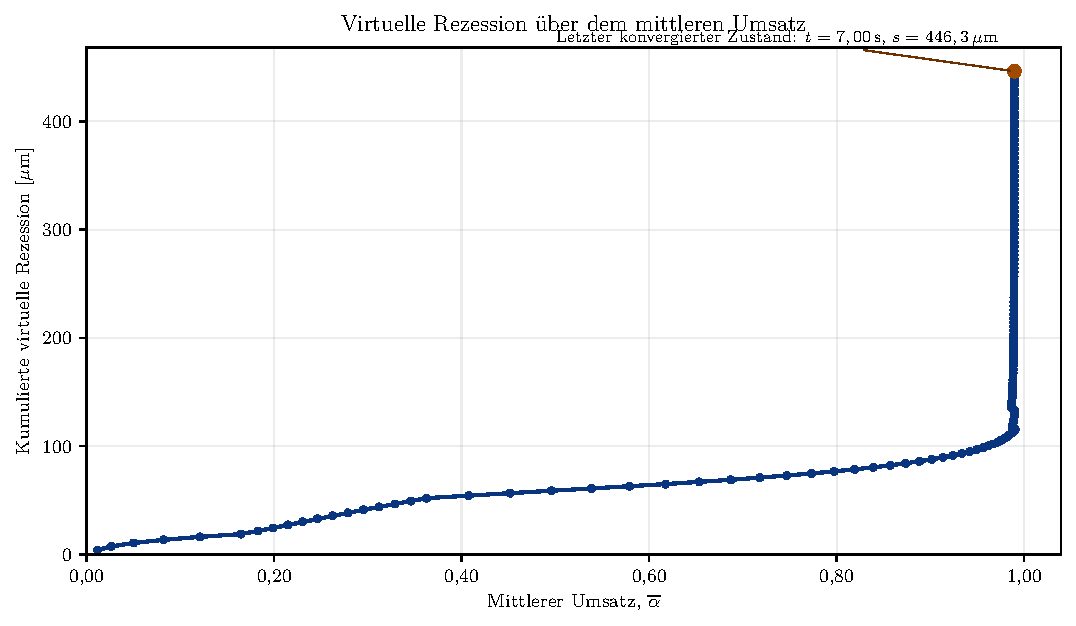
\includegraphics[width=0.96\textwidth]{../analysis/simulation3_sector_recession_vs_alpha_avg_de.pdf}
\caption{Akkumulierte virtuelle Rezession versus Mittelwert der aktiven Schicht.}
\label{fig:sim3-recession-alpha-de}
\end{figure}

\begin{figure}[H]
\centering
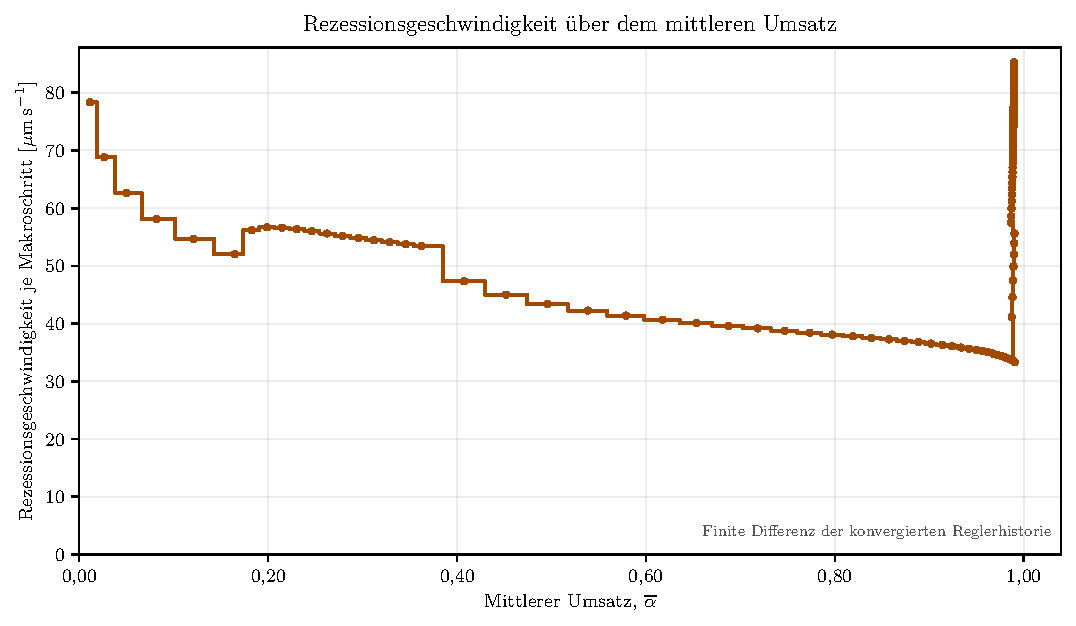
\includegraphics[width=0.96\textwidth]{../analysis/simulation3_sector_recession_rate_vs_alpha_avg_de.pdf}
\caption{Makroschritt-Rezessionsrate versus Mittelwert-Umrechnung.}
\label{fig:sim3-rate-alpha-de}
\end{figure}

\subsection{Endgültige räumliche Analyse von Zustandsvariablen}

Nach normaler Fertigstellung wurden die zehn \code{file0.rth} bis \code{file9.rth} Partitionen im streng zerstörungsfreien Modus gelesen. Alle 140 DPF-Zeiten stimmen genau mit den 140 Verlaufszeiten überein. Element-Node-Beiträge, die sich eine globale Knotenkennung teilen, werden über Elemente und Partitionen gemittelt und dann in 100 Radialbändern von 1\% gruppiert. Der Extraktor behandelt die Topologie jedes Staates separat, so dass Profile nach beiden Löschereignissen gültig bleiben.

Die Konturen von 90\%, 95\% und 99\% erscheinen zuerst bei \SI{1.80}{s}, \SI{2.05}{s} und \SI{2.55}{s}. Bei \SI{7.00}{s} sind ihre Tiefen vom anfänglichen heißen Gesicht \SI{0.223066}{mm}, \SI{0.156483}{mm} und \SI{0.048842}{mm}. Die signierten Trennungen \(d_\alpha-s\) sind daher \SI{-0.223188}{mm}, \SI{-0.289771}{mm} und \SI{-0.397412}{mm}. Die energiebasierte virtuelle Rezessionskoordinate ist somit tiefer als alle drei Umwandlungsfronten, was bestätigt, dass sie nicht als \code{SVAR1} Kontur interpretiert werden darf.

\begin{figure}[H]
\centering
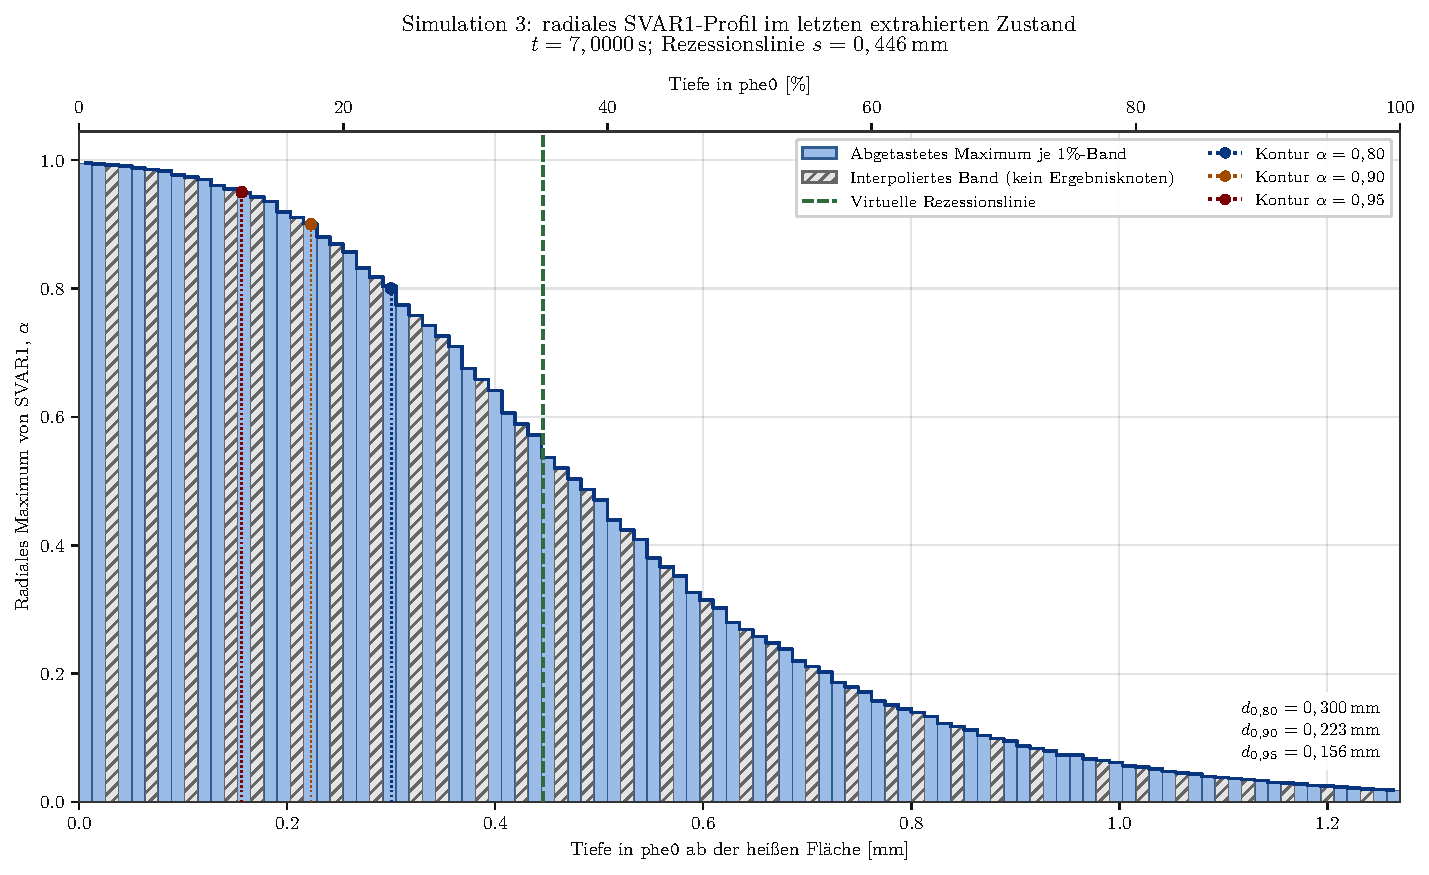
\includegraphics[width=0.96\textwidth]{../analysis/simulation3_sector_svar1_radial_profile_1pct_de.pdf}
\caption{ Endgültiges radiales \code{SVAR1} Profil bei \SI{7}{s}, einschließlich Umrechnungskonturen und der virtuellen Rezessionslinie.}
\label{fig:sim3-svar1-radial-final-de}
\end{figure}

\begin{figure}[H]
\centering
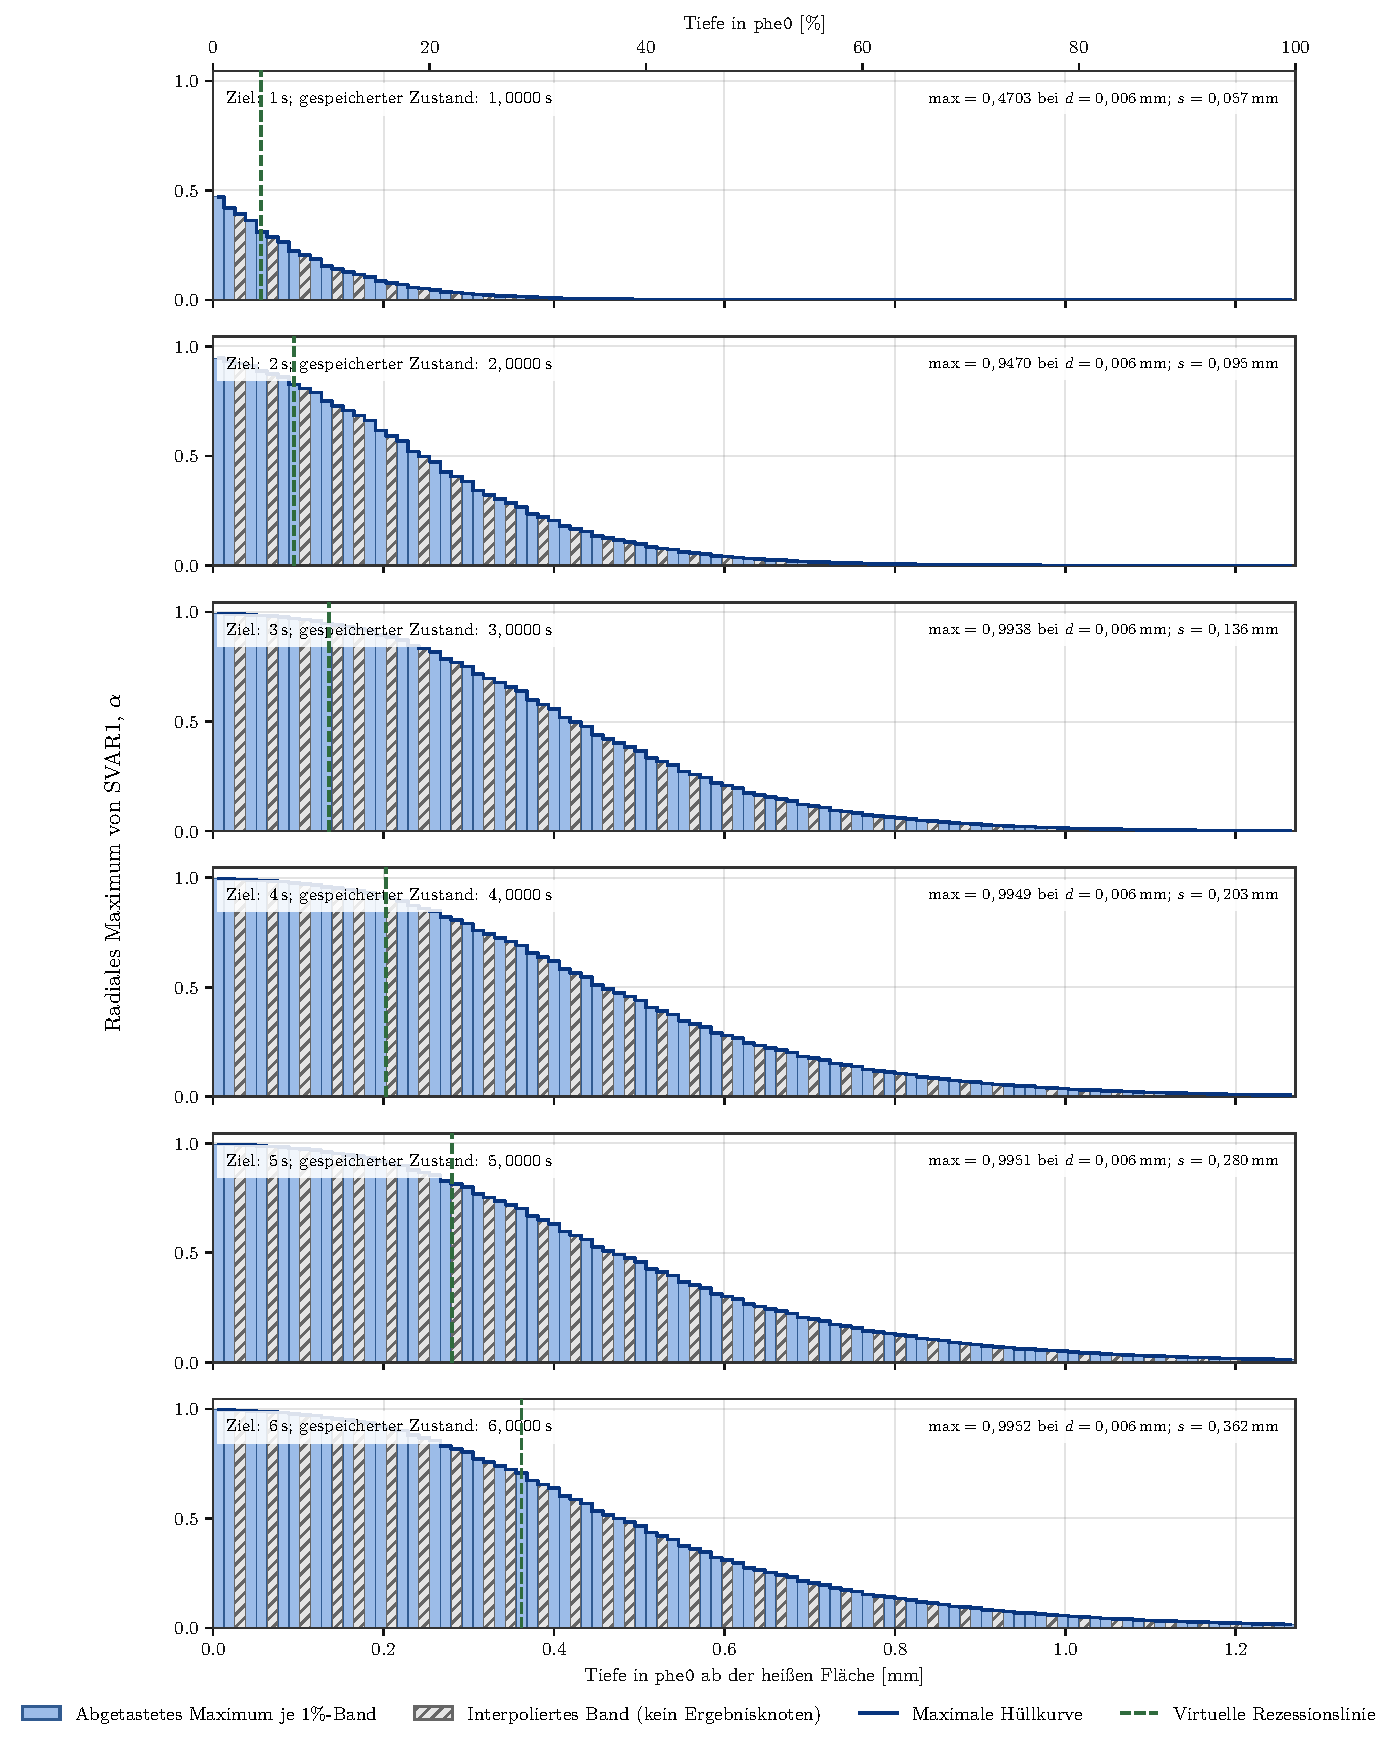
\includegraphics[width=0.86\textwidth]{../analysis/simulation3_sector_svar1_radial_time_profiles_1pct_de.pdf}
\caption{Entwicklung von radialen \code{SVAR1} Profilen von 1 zu \SI{6}{s}. Die Rezessionslinie wird in jedem Panel angezeigt.}
\label{fig:sim3-svar1-radial-time-de}
\end{figure}

\begin{figure}[H]
\centering
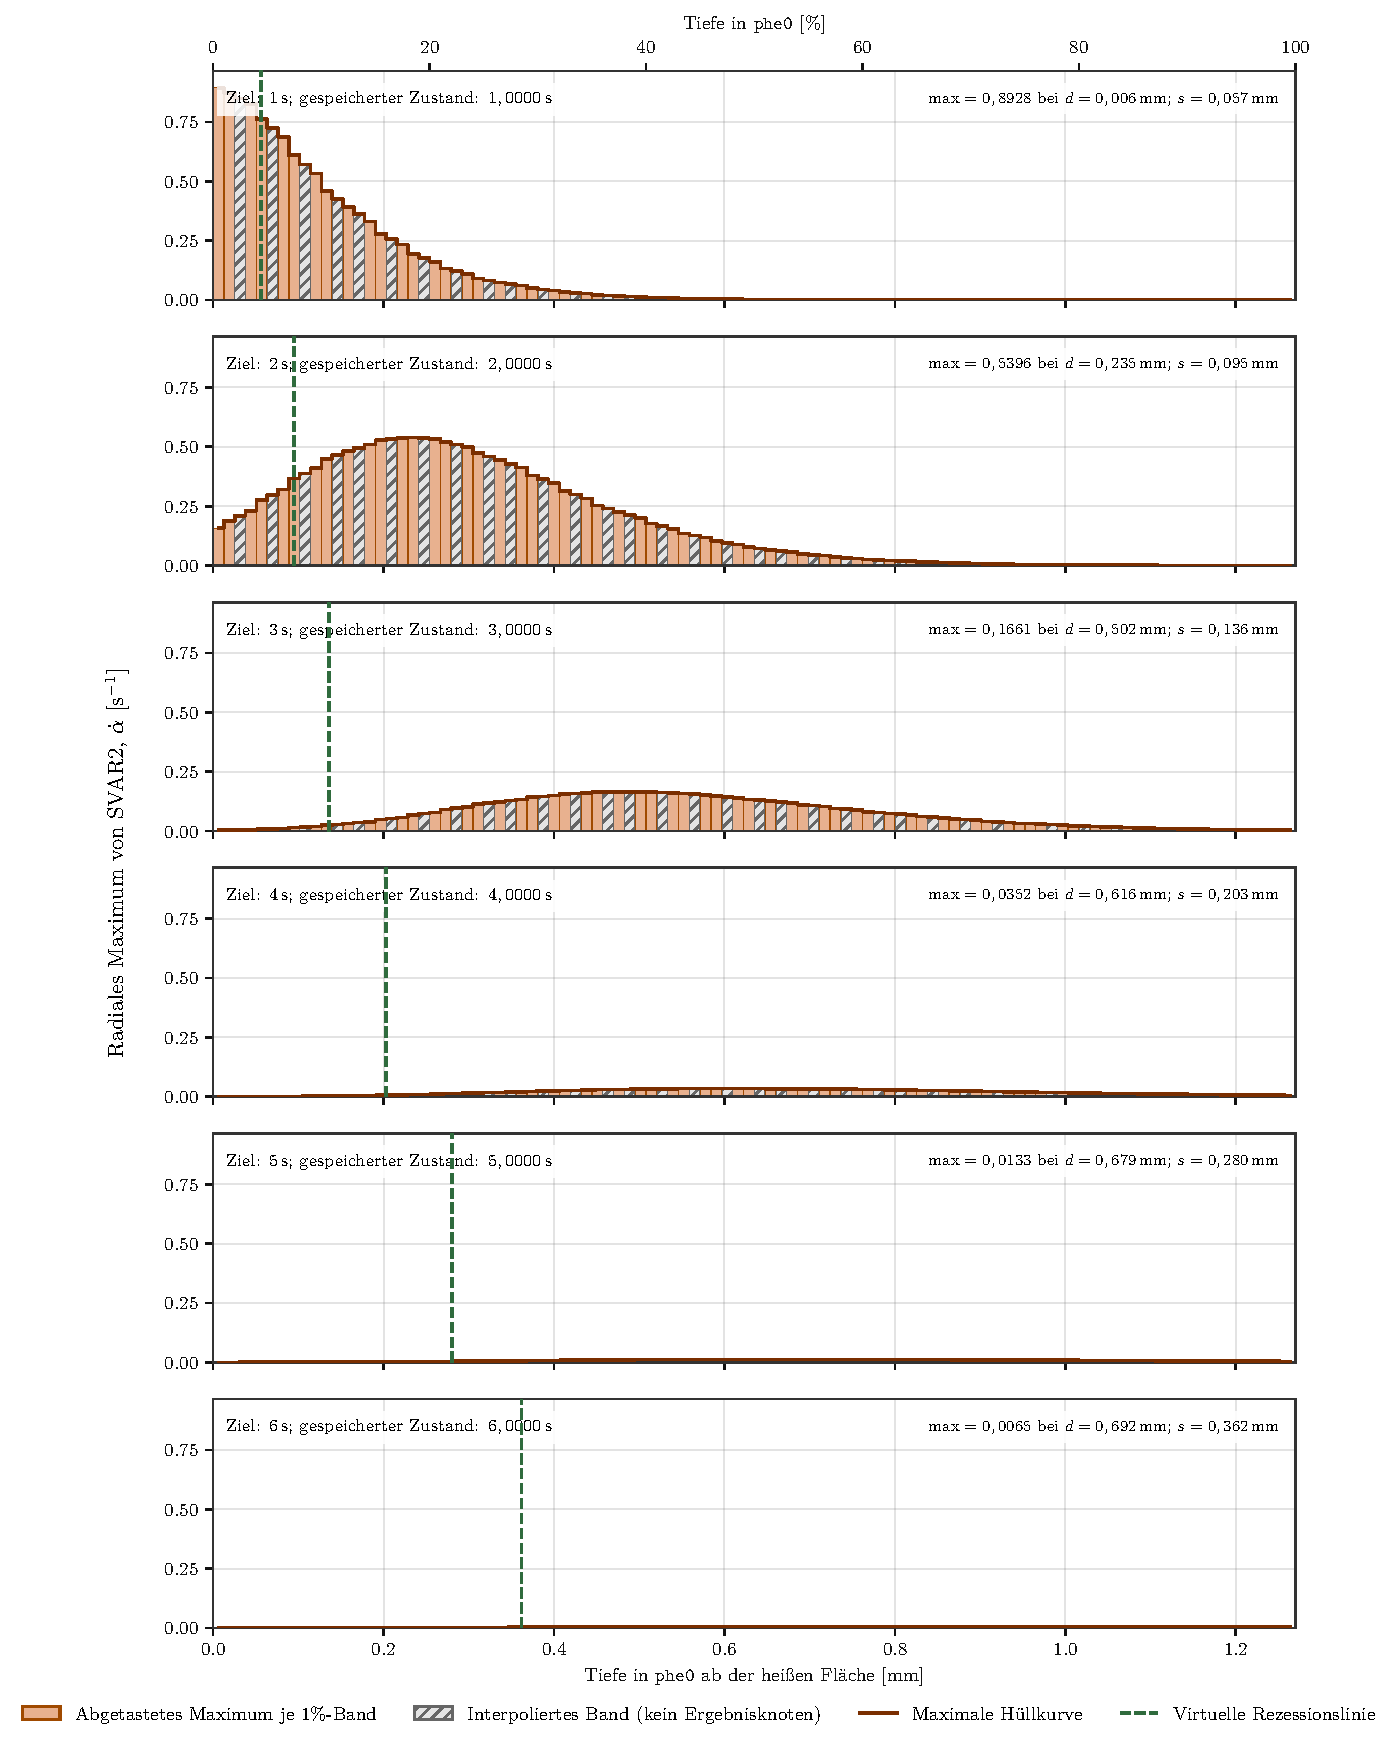
\includegraphics[width=0.86\textwidth]{../analysis/simulation3_sector_svar2_radial_time_profiles_1pct_de.pdf}
\caption{Entwicklung von radialen \code{SVAR2} Profilen; das Maximum identifiziert den Bereich, in dem die Pyrolyse aktiv bleibt.}
\label{fig:sim3-svar2-radial-time-de}
\end{figure}

\begin{figure}[H]
\centering
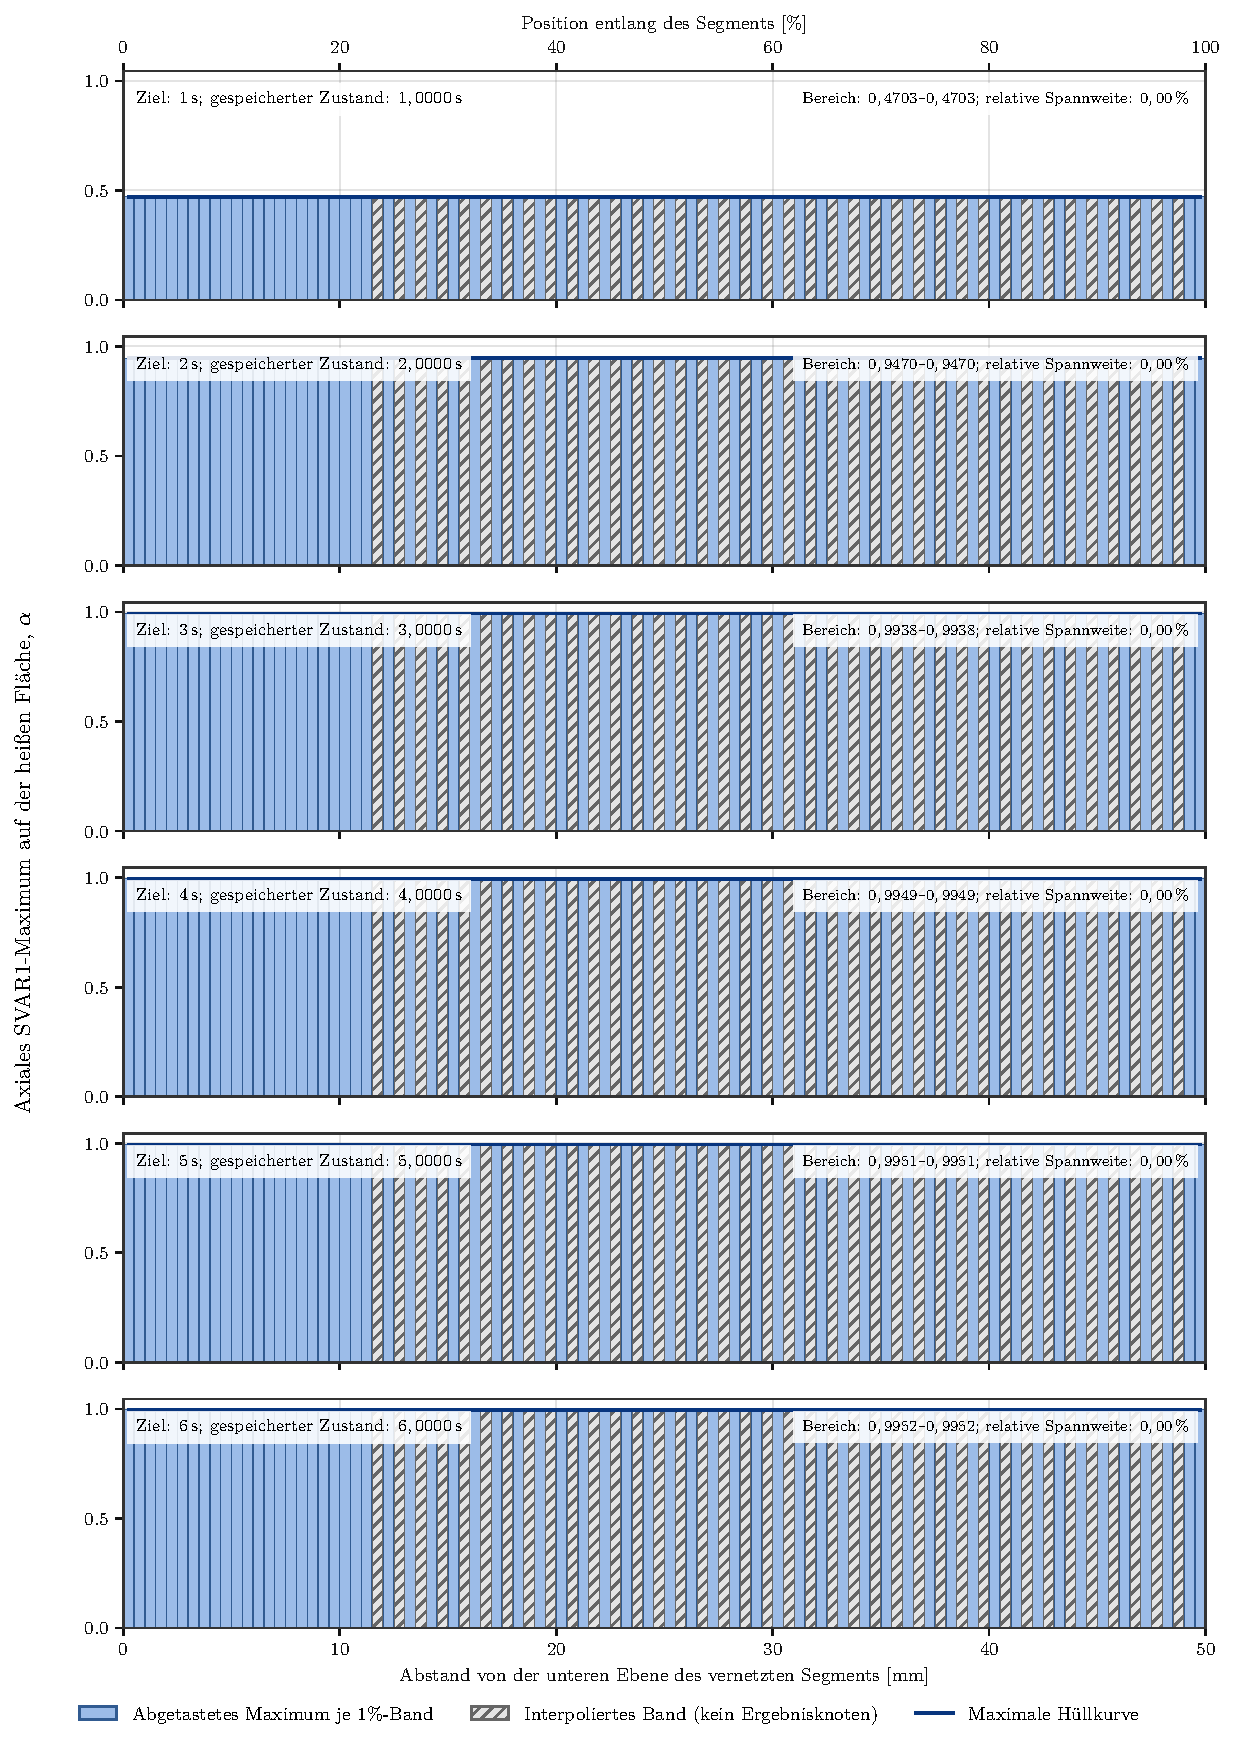
\includegraphics[width=0.86\textwidth]{../analysis/simulation3_sector_svar1_axial_time_profiles_1pct_de.pdf}
\caption{Axiale Einheitlichkeit von \code{SVAR1} entlang des heißen Gesichts des dünnen Sektors.}
\label{fig:sim3-svar1-axial-time-de}
\end{figure}

\begin{figure}[H]
\centering
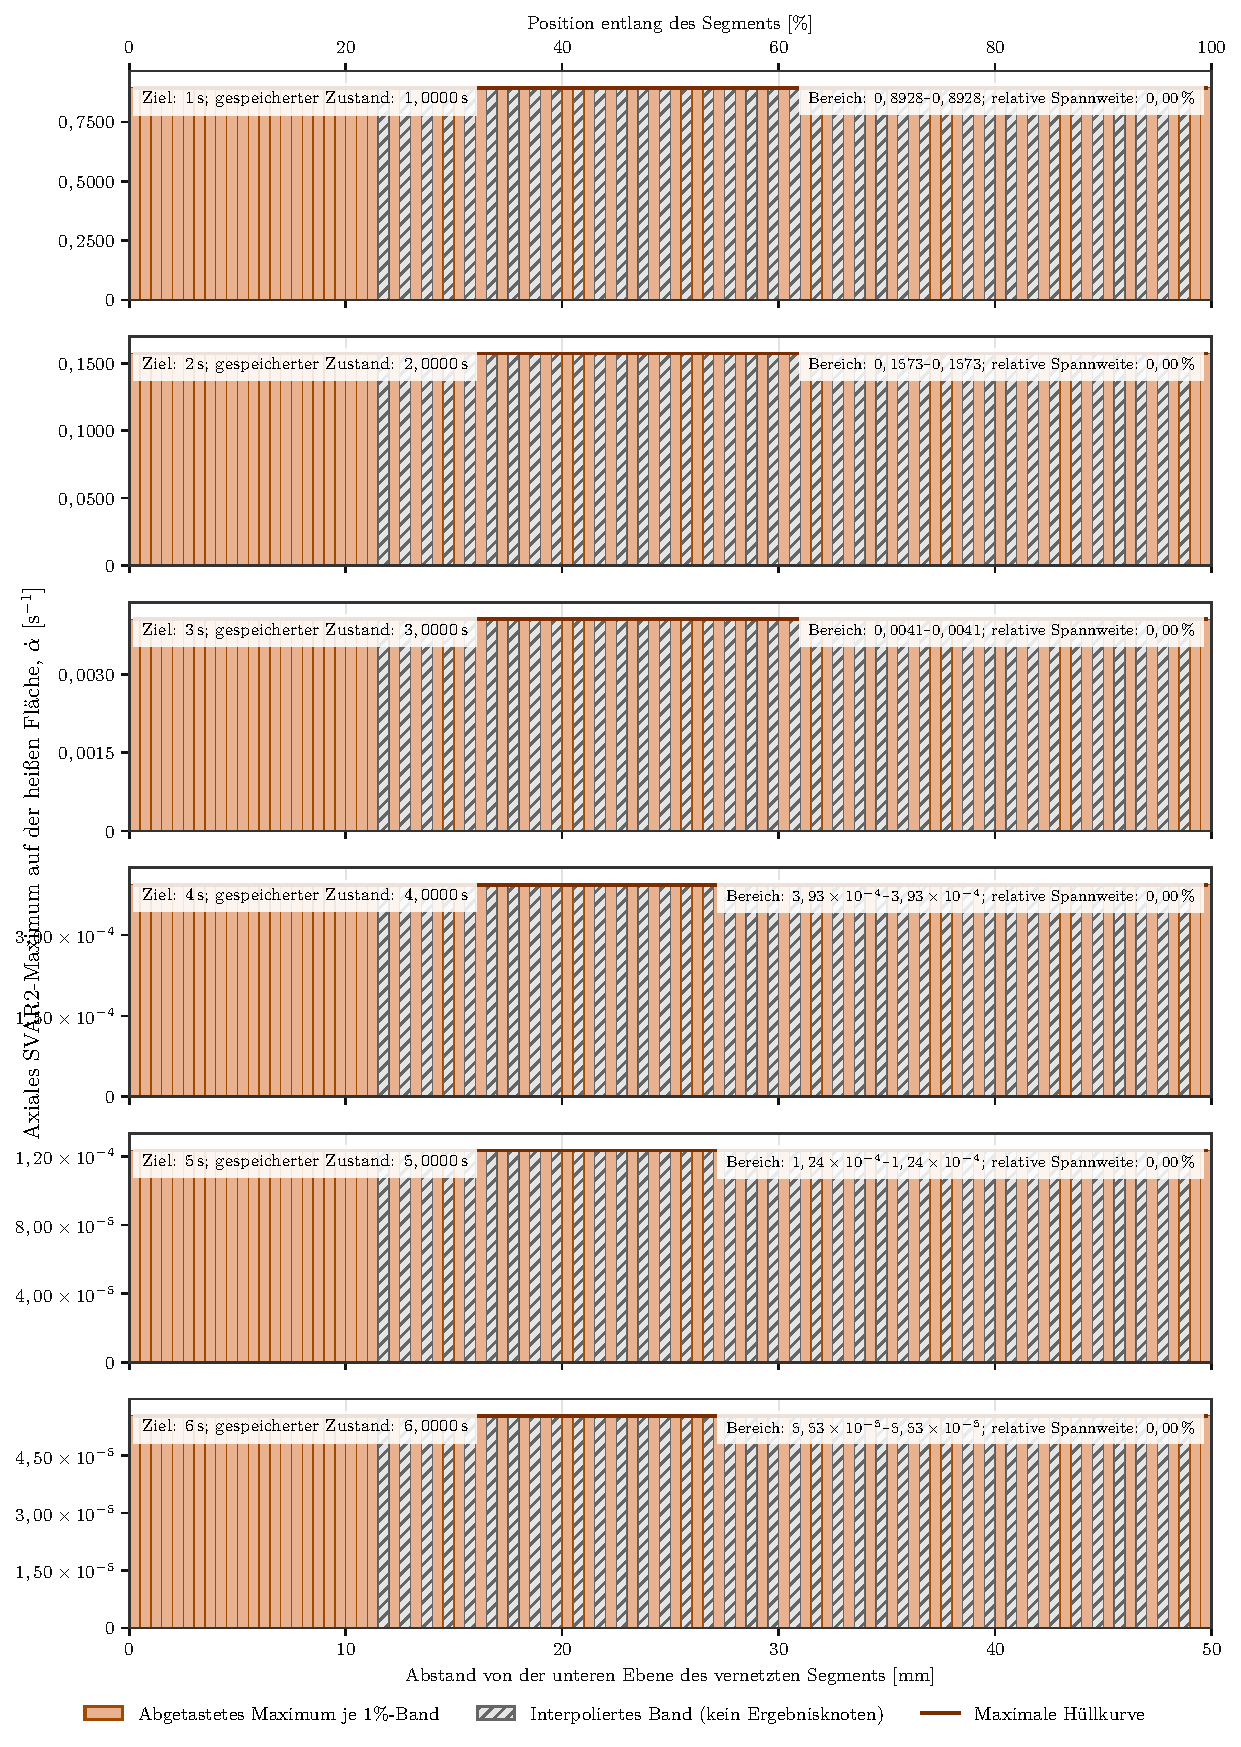
\includegraphics[width=0.86\textwidth]{../analysis/simulation3_sector_svar2_axial_time_profiles_1pct_de.pdf}
\caption{Axiale Einheitlichkeit von \code{SVAR2} entlang des heißen Gesichts des dünnen Sektors.}
\label{fig:sim3-svar2-axial-time-de}
\end{figure}

\begin{figure}[H]
\centering
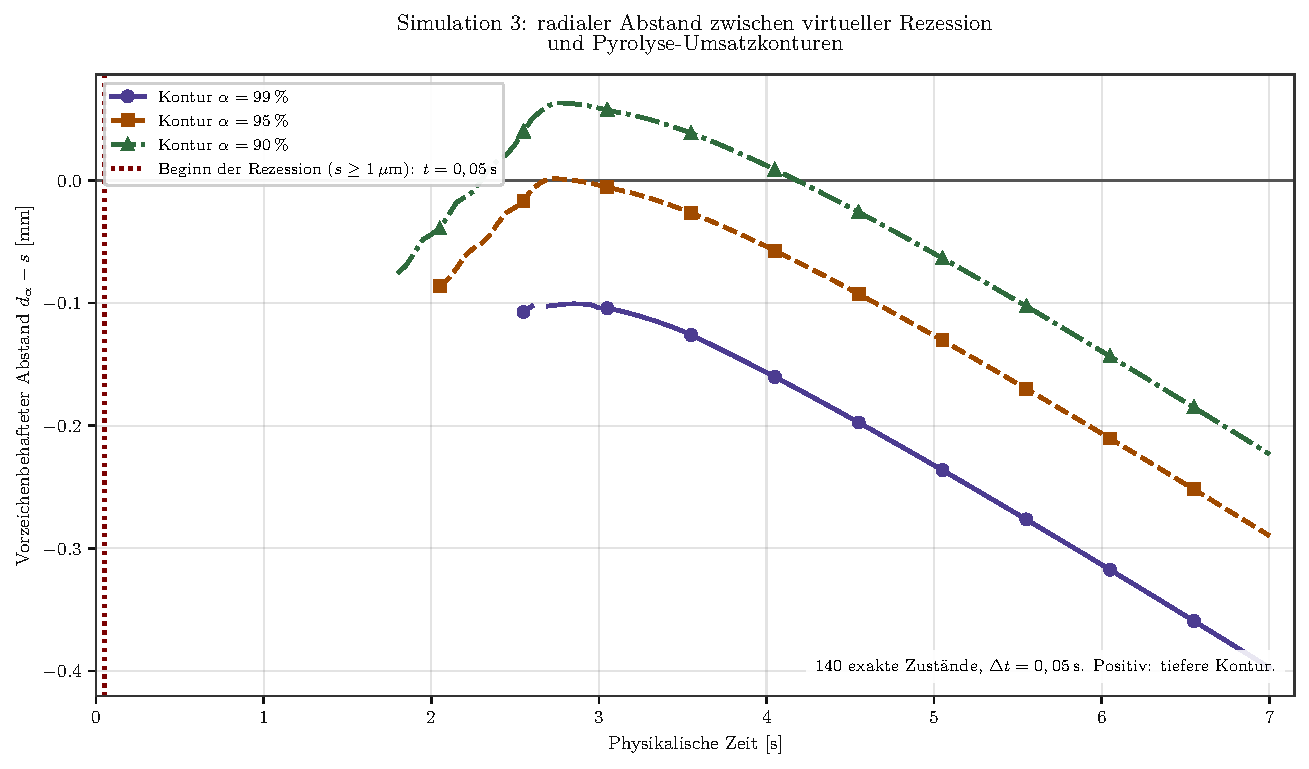
\includegraphics[width=0.96\textwidth]{../analysis/simulation3_sector_recession_to_pyrolysis_contours_vs_time_de.pdf}
\caption{Signierte Trennung zwischen der Rezessionslinie und den 99\%, 95\%, und 90\% Umrechnungskonturen über alle 140 Zustände. Positive Werte legen die Kontur tiefer in die Wand. Die vertikale Linie markiert die erste numerisch signifikante Rezession.}
\label{fig:sim3-recession-contour-distance-de}
\end{figure}

\subsection{Anwendungsbereich und Reproduzierbarkeit}

Die Kampagne Simulation 3 wird unter \SI{7}{s} geschlossen. Zeitliche Ergebnisse stammen aus der synchronisierten endgültigen Historie und räumliche Ergebnisse aus den zehn stabilen RTH-Partitionen. Schlussfolgerungen bleiben abhängig von den materiellen Gesetzen, der Extrapolation von Niedrigtemperatureigenschaften und den numerischen Kriterien \(\alpha_c=0.99\) und \(\Delta r=\SI{19.84375}{\micro m}\). Sie stellen für sich genommen keine experimentelle Validierung der Ablation dar. Alle CSV-Dateien und zweisprachigen Zahlen in diesem Abschnitt können aus den erhaltenen Endergebnisdateien reproduziert werden.

% ============================================================================
\clearpage
\renewcommand{\refname}{Literatur}
\renewcommand{\bibname}{Literatur}
\begin{thebibliography}{99}

\bibitem{ansys-usermatth}
ANSYS, Inc., \emph{UserMatTh --- User-Defined Thermal Material Model},
Mechanical APDL Programmer's Reference, version 2026 R1,
\url{https://ansyshelp.ansys.com/public/Views/Secured/corp/v261/en/ans_prog/Z7K4r1e5lcd.html},
accessed July 15, 2026.

\bibitem{ansys-birthdeath}
ANSYS, Inc., \emph{Using Element Birth and Death}, Mechanical APDL Advanced
Analysis Guide,
\url{https://ansyshelp.ansys.com/public/Views/Secured/corp/v251/en/ans_adv/Hlp_G_ADV6_2.html},
accessed July 15, 2026.

\bibitem{ansys-ekill}
ANSYS, Inc., \emph{EKILL --- Deactivates an element}, Mechanical APDL Command
Reference,
\url{https://ansyshelp.ansys.com/public/Views/Secured/corp/v242/en/ans_cmd/Hlp_C_EKILL.html},
accessed July 15, 2026.

\bibitem{ewing2013}
M. E. Ewing, T. S. Laker, and D. T. Walker, \emph{Numerical Modeling of
Ablation Heat Transfer}, NASA NTRS 20140008557, 2013,
\url{https://ntrs.nasa.gov/citations/20140008557}.

\bibitem{amar2010}
A. J. Amar, N. D. Calvert, and B. S. Kirk, \emph{Development and Verification of
the Charring Ablating Thermal Protection Implicit System Solver}, NASA NTRS
20110000471, 2010,
\url{https://ntrs.nasa.gov/citations/20110000471}.

\bibitem{amar2016}
A. J. Amar, A. B. Oliver, B. S. Kirk, G. Salazar, and J. Droba,
\emph{Overview of the CHarring Ablator Response (CHAR) Code}, NASA NTRS
20160005889, 2016,
\url{https://ntrs.nasa.gov/citations/20160005889}.

\bibitem{clark1972}
R. K. Clark, \emph{A Numerical Analysis of the Transient Response of an
Ablation System Including Effects of Thermal Nonequilibrium, Mass Transfer and
Chemical Kinetics}, NASA-TM-X-68853, NASA NTRS 19730002381, 1972,
\url{https://ntrs.nasa.gov/citations/19730002381}.

\bibitem{bessire2023}
B. K. Bessire, \emph{Analysis of Pyrolysis Products from Ablative TPS}, NASA
NTRS 20230000843, 2023,
\url{https://ntrs.nasa.gov/citations/20230000843}.

\bibitem{nasa-testing}
NASA Ames Research Center, \emph{Thermal Protection Materials Branch ---
Testing and Fabrication}, description of TGA, DSC, and LFA measurements,
\url{https://www.nasa.gov/thermal-protection-materials-branch-testing-and-fabrication/},
accessed July 15, 2026.

\bibitem{local-step}
MIT Rocket Team, \code{motoren.stp}, project AP214 STEP geometry, local file
analyzed July 15, 2026.

\bibitem{local-model}
MIT Rocket Team, \code{EngineeringData.xml}, \code{ds.dat},
\code{phenolic_pyrolysis_native.apdl}, and \code{usermatth.F}, local artifacts
from the ANSYS Mechanical 2026 R1 simulation, state analyzed July 15, 2026.

\bibitem{local-results}
MIT Rocket Team, \code{file0.rth}--\code{file7.rth}, \code{file.nlh},
\code{file.mntr}, \code{solve.out}, and
\code{svar1_radial_profile_1pct.csv}, local outputs from the ANSYS Mechanical
2026 R1 simulation, last converged state at \(t=\SI{6.38561694}{s}\), analyzed
July 16, 2026.

\end{thebibliography}

\clearpage
\renewcommand{\listfigurename}{Abbildungsverzeichnis}
\renewcommand{\listtablename}{Tabellenverzeichnis}
\listoffigures
\listoftables

\vfill
\section*{AI Nutzungserklärung}

Künstliche Intelligenz wurde verwendet, um Teile dieses Dokuments zu generieren und einen Teil seiner technischen Inhaltsentwicklung zu unterstützen.
\end{document}
